\documentclass[twoside]{book}

% Packages required by doxygen
\usepackage{fixltx2e}
\usepackage{calc}
\usepackage{doxygen}
\usepackage[export]{adjustbox} % also loads graphicx
\usepackage{graphicx}
\usepackage[utf8]{inputenc}
\usepackage{makeidx}
\usepackage{multicol}
\usepackage{multirow}
\PassOptionsToPackage{warn}{textcomp}
\usepackage{textcomp}
\usepackage[nointegrals]{wasysym}
\usepackage[table]{xcolor}

% Font selection
\usepackage[T1]{fontenc}
\usepackage[scaled=.90]{helvet}
\usepackage{courier}
\usepackage{amssymb}
\usepackage{sectsty}
\renewcommand{\familydefault}{\sfdefault}
\allsectionsfont{%
  \fontseries{bc}\selectfont%
  \color{darkgray}%
}
\renewcommand{\DoxyLabelFont}{%
  \fontseries{bc}\selectfont%
  \color{darkgray}%
}
\newcommand{\+}{\discretionary{\mbox{\scriptsize$\hookleftarrow$}}{}{}}

% Page & text layout
\usepackage{geometry}
\geometry{%
  a4paper,%
  top=2.5cm,%
  bottom=2.5cm,%
  left=2.5cm,%
  right=2.5cm%
}
\tolerance=750
\hfuzz=15pt
\hbadness=750
\setlength{\emergencystretch}{15pt}
\setlength{\parindent}{0cm}
\setlength{\parskip}{3ex plus 2ex minus 2ex}
\makeatletter
\renewcommand{\paragraph}{%
  \@startsection{paragraph}{4}{0ex}{-1.0ex}{1.0ex}{%
    \normalfont\normalsize\bfseries\SS@parafont%
  }%
}
\renewcommand{\subparagraph}{%
  \@startsection{subparagraph}{5}{0ex}{-1.0ex}{1.0ex}{%
    \normalfont\normalsize\bfseries\SS@subparafont%
  }%
}
\makeatother

% Headers & footers
\usepackage{fancyhdr}
\pagestyle{fancyplain}
\fancyhead[LE]{\fancyplain{}{\bfseries\thepage}}
\fancyhead[CE]{\fancyplain{}{}}
\fancyhead[RE]{\fancyplain{}{\bfseries\leftmark}}
\fancyhead[LO]{\fancyplain{}{\bfseries\rightmark}}
\fancyhead[CO]{\fancyplain{}{}}
\fancyhead[RO]{\fancyplain{}{\bfseries\thepage}}
\fancyfoot[LE]{\fancyplain{}{}}
\fancyfoot[CE]{\fancyplain{}{}}
\fancyfoot[RE]{\fancyplain{}{\bfseries\scriptsize Generated by Doxygen }}
\fancyfoot[LO]{\fancyplain{}{\bfseries\scriptsize Generated by Doxygen }}
\fancyfoot[CO]{\fancyplain{}{}}
\fancyfoot[RO]{\fancyplain{}{}}
\renewcommand{\footrulewidth}{0.4pt}
\renewcommand{\chaptermark}[1]{%
  \markboth{#1}{}%
}
\renewcommand{\sectionmark}[1]{%
  \markright{\thesection\ #1}%
}

% Indices & bibliography
\usepackage{natbib}
\usepackage[titles]{tocloft}
\setcounter{tocdepth}{3}
\setcounter{secnumdepth}{5}
\makeindex

% Hyperlinks (required, but should be loaded last)
\usepackage{ifpdf}
\ifpdf
  \usepackage[pdftex,pagebackref=true]{hyperref}
\else
  \usepackage[ps2pdf,pagebackref=true]{hyperref}
\fi
\hypersetup{%
  colorlinks=true,%
  linkcolor=blue,%
  citecolor=blue,%
  unicode%
}

% Custom commands
\newcommand{\clearemptydoublepage}{%
  \newpage{\pagestyle{empty}\cleardoublepage}%
}

\usepackage{caption}
\captionsetup{labelsep=space,justification=centering,font={bf},singlelinecheck=off,skip=4pt,position=top}

%===== C O N T E N T S =====

\begin{document}

% Titlepage & ToC
\hypersetup{pageanchor=false,
             bookmarksnumbered=true,
             pdfencoding=unicode
            }
\pagenumbering{roman}
\begin{titlepage}
\vspace*{7cm}
\begin{center}%
{\Large D\+TV App }\\
\vspace*{1cm}
{\large Generated by Doxygen 1.8.11}\\
\end{center}
\end{titlepage}
\clearemptydoublepage
\tableofcontents
\clearemptydoublepage
\pagenumbering{arabic}
\hypersetup{pageanchor=true}

%--- Begin generated contents ---
\chapter{Module Index}
\section{Modules}
Here is a list of all modules\+:\begin{DoxyCompactList}
\item \contentsline{section}{Configuration file interface}{\pageref{group__config}}{}
\item \contentsline{section}{Drawing interface}{\pageref{group__drawing}}{}
\item \contentsline{section}{D\+TV interface}{\pageref{group__dtv}}{}
\item \contentsline{section}{Graphics interface}{\pageref{group__graphics}}{}
\item \contentsline{section}{Table parsing interface}{\pageref{group__parsing}}{}
\item \contentsline{section}{Remote-\/control interface}{\pageref{group__rc}}{}
\item \contentsline{section}{D\+VB table retrieval interface}{\pageref{group__structure}}{}
\end{DoxyCompactList}

\chapter{Data Structure Index}
\section{Data Structures}
Here are the data structures with brief descriptions\+:\begin{DoxyCompactList}
\item\contentsline{section}{\hyperlink{structconfig__init__ch__info}{config\+\_\+init\+\_\+ch\+\_\+info} \\*A structure that holds the initial dtv settings }{\pageref{structconfig__init__ch__info}}{}
\item\contentsline{section}{\hyperlink{structdraw__interface}{draw\+\_\+interface} \\*Basic interface necessary to display graphics elements }{\pageref{structdraw__interface}}{}
\item\contentsline{section}{\hyperlink{structdtv__channel__info}{dtv\+\_\+channel\+\_\+info} \\*Contains basic channel info }{\pageref{structdtv__channel__info}}{}
\item\contentsline{section}{\hyperlink{structgraphics__args}{graphics\+\_\+args} \\*A shim structure to pass main arguments to Direct\+FB }{\pageref{structgraphics__args}}{}
\item\contentsline{section}{\hyperlink{structgraphics__channel__info}{graphics\+\_\+channel\+\_\+info} \\*A struct that contains some basic channel info }{\pageref{structgraphics__channel__info}}{}
\item\contentsline{section}{\hyperlink{structgraphics__flags}{graphics\+\_\+flags} \\*A struct that keeps the state of what should be displayed }{\pageref{structgraphics__flags}}{}
\item\contentsline{section}{\hyperlink{structpat}{pat} \\*Contains important info from the P\+AT table }{\pageref{structpat}}{}
\item\contentsline{section}{\hyperlink{structpat__body}{pat\+\_\+body} \\*Represents P\+AT body }{\pageref{structpat__body}}{}
\item\contentsline{section}{\hyperlink{structpat__header}{pat\+\_\+header} \\*Represents P\+AT header }{\pageref{structpat__header}}{}
\item\contentsline{section}{\hyperlink{structpmt}{pmt} \\*Contains important info from the P\+MT table }{\pageref{structpmt}}{}
\item\contentsline{section}{\hyperlink{structpat_1_1pmt__basic}{pat\+::pmt\+\_\+basic} \\*Contains enough info to identify a P\+MT table }{\pageref{structpat_1_1pmt__basic}}{}
\item\contentsline{section}{\hyperlink{structpmt__body}{pmt\+\_\+body} \\*Represents P\+MT body }{\pageref{structpmt__body}}{}
\item\contentsline{section}{\hyperlink{structpmt__header}{pmt\+\_\+header} \\*Represents P\+MT header }{\pageref{structpmt__header}}{}
\item\contentsline{section}{\hyperlink{structrc__args}{rc\+\_\+args} \\*A shim structure to pass arguments to event thread }{\pageref{structrc__args}}{}
\item\contentsline{section}{\hyperlink{structsdt}{sdt} \\*Contains important info from the S\+DT table }{\pageref{structsdt}}{}
\item\contentsline{section}{\hyperlink{structsdt__body}{sdt\+\_\+body} \\*Represents S\+DT body }{\pageref{structsdt__body}}{}
\item\contentsline{section}{\hyperlink{structsdt__descriptor1}{sdt\+\_\+descriptor1} \\*Represents the first half of the service descriptor }{\pageref{structsdt__descriptor1}}{}
\item\contentsline{section}{\hyperlink{structsdt__descriptor2}{sdt\+\_\+descriptor2} \\*Represents the second half of the service descriptor }{\pageref{structsdt__descriptor2}}{}
\item\contentsline{section}{\hyperlink{structsdt__header}{sdt\+\_\+header} \\*Represents S\+DT header }{\pageref{structsdt__header}}{}
\item\contentsline{section}{\hyperlink{structtable__header}{table\+\_\+header} \\*Header that is part of all tables }{\pageref{structtable__header}}{}
\item\contentsline{section}{\hyperlink{structteletext__descriptor__header}{teletext\+\_\+descriptor\+\_\+header} \\*Represents the teletext descriptor header }{\pageref{structteletext__descriptor__header}}{}
\item\contentsline{section}{\hyperlink{structtot__descriptor__body}{tot\+\_\+descriptor\+\_\+body} \\*Represents T\+OT descriptor body }{\pageref{structtot__descriptor__body}}{}
\item\contentsline{section}{\hyperlink{structtot__descriptor__header}{tot\+\_\+descriptor\+\_\+header} \\*Represents T\+OT descriptor header }{\pageref{structtot__descriptor__header}}{}
\item\contentsline{section}{\hyperlink{structtot__header}{tot\+\_\+header} \\*Represents T\+OT header }{\pageref{structtot__header}}{}
\end{DoxyCompactList}

\chapter{File Index}
\section{File List}
Here is a list of all documented files with brief descriptions\+:\begin{DoxyCompactList}
\item\contentsline{section}{include/\hyperlink{common_8h}{common.\+h} \\*Contains functions that all modules use }{\pageref{common_8h}}{}
\item\contentsline{section}{include/\hyperlink{config_8h}{config.\+h} \\*Contains configuration file A\+PI }{\pageref{config_8h}}{}
\item\contentsline{section}{include/\hyperlink{drawing_8h}{drawing.\+h} \\*Contains A\+PI for drawing graphics elements }{\pageref{drawing_8h}}{}
\item\contentsline{section}{include/\hyperlink{dtv_8h}{dtv.\+h} \\*Contains D\+TV A\+PI }{\pageref{dtv_8h}}{}
\item\contentsline{section}{include/\hyperlink{graphics_8h}{graphics.\+h} \\*Contains the graphics A\+PI }{\pageref{graphics_8h}}{}
\item\contentsline{section}{include/\hyperlink{parsing_8h}{parsing.\+h} \\*Contains streamlined internal representations of tables }{\pageref{parsing_8h}}{}
\item\contentsline{section}{include/\hyperlink{rc_8h}{rc.\+h} \\*Contains Remote Control A\+PI }{\pageref{rc_8h}}{}
\item\contentsline{section}{include/\hyperlink{structures_8h}{structures.\+h} \\*Contains nitty-\/gritty D\+VB details }{\pageref{structures_8h}}{}
\item\contentsline{section}{src/\hyperlink{config_8c}{config.\+c} \\*Implementation for the configuration file interface }{\pageref{config_8c}}{}
\item\contentsline{section}{src/\hyperlink{graphics_8c}{graphics.\+c} \\*Contains implementation for graphics interface }{\pageref{graphics_8c}}{}
\item\contentsline{section}{src/\hyperlink{main_8c}{main.\+c} \\*Contains the implementation that glues other modules together }{\pageref{main_8c}}{}
\item\contentsline{section}{src/\hyperlink{rc_8c}{rc.\+c} \\*Contains the implementation of the remote control interface }{\pageref{rc_8c}}{}
\end{DoxyCompactList}

\chapter{Module Documentation}
\hypertarget{group__config}{}\section{Configuration file interface}
\label{group__config}\index{Configuration file interface@{Configuration file interface}}


Functions and structures for retrieveing configuration options.  


\subsection*{Data Structures}
\begin{DoxyCompactItemize}
\item 
struct \hyperlink{structconfig__init__ch__info}{config\+\_\+init\+\_\+ch\+\_\+info}
\begin{DoxyCompactList}\small\item\em A structure that holds the initial dtv settings. \end{DoxyCompactList}\end{DoxyCompactItemize}
\subsection*{Functions}
\begin{DoxyCompactItemize}
\item 
struct \hyperlink{structconfig__init__ch__info}{config\+\_\+init\+\_\+ch\+\_\+info} \hyperlink{group__config_gad7d820530151b1bb2b6cf6e992f48331}{config\+\_\+get\+\_\+init\+\_\+ch\+\_\+info} (F\+I\+LE $\ast$f)
\begin{DoxyCompactList}\small\item\em Reads the initial settings from the specified file. \end{DoxyCompactList}\end{DoxyCompactItemize}


\subsection{Detailed Description}
Functions and structures for retrieveing configuration options. 



\subsection{Function Documentation}
\index{Configuration file interface@{Configuration file interface}!config\+\_\+get\+\_\+init\+\_\+ch\+\_\+info@{config\+\_\+get\+\_\+init\+\_\+ch\+\_\+info}}
\index{config\+\_\+get\+\_\+init\+\_\+ch\+\_\+info@{config\+\_\+get\+\_\+init\+\_\+ch\+\_\+info}!Configuration file interface@{Configuration file interface}}
\subsubsection[{\texorpdfstring{config\+\_\+get\+\_\+init\+\_\+ch\+\_\+info(\+F\+I\+L\+E $\ast$f)}{config_get_init_ch_info(FILE *f)}}]{\setlength{\rightskip}{0pt plus 5cm}struct {\bf config\+\_\+init\+\_\+ch\+\_\+info} config\+\_\+get\+\_\+init\+\_\+ch\+\_\+info (
\begin{DoxyParamCaption}
\item[{F\+I\+LE $\ast$}]{f}
\end{DoxyParamCaption}
)}\hypertarget{group__config_gad7d820530151b1bb2b6cf6e992f48331}{}\label{group__config_gad7d820530151b1bb2b6cf6e992f48331}


Reads the initial settings from the specified file. 

Reads the initial settings from the specified file. 
\hypertarget{group__drawing}{}\section{Drawing interface}
\label{group__drawing}\index{Drawing interface@{Drawing interface}}


Functions and structures for drawing.  


\subsection*{Data Structures}
\begin{DoxyCompactItemize}
\item 
struct \hyperlink{structdraw__interface}{draw\+\_\+interface}
\begin{DoxyCompactList}\small\item\em Basic interface necessary to display graphics elements. \end{DoxyCompactList}\end{DoxyCompactItemize}
\subsection*{Functions}
\begin{DoxyCompactItemize}
\item 
int32\+\_\+t \hyperlink{group__drawing_ga50526d5e4e244599996608371f410bf2}{draw\+\_\+init} (struct \hyperlink{structdraw__interface}{draw\+\_\+interface} $\ast$draw\+\_\+i, int $\ast$argc, char $\ast$$\ast$$\ast$argv)\hypertarget{group__drawing_ga50526d5e4e244599996608371f410bf2}{}\label{group__drawing_ga50526d5e4e244599996608371f410bf2}

\begin{DoxyCompactList}\small\item\em Initialize drawing interface. \end{DoxyCompactList}\item 
int32\+\_\+t \hyperlink{group__drawing_ga71818ed76471623e9aeffe07a0ba26d2}{draw\+\_\+channel\+\_\+info} (struct \hyperlink{structdraw__interface}{draw\+\_\+interface} $\ast$draw\+\_\+i, struct \hyperlink{structgraphics__channel__info}{graphics\+\_\+channel\+\_\+info} info)\hypertarget{group__drawing_ga71818ed76471623e9aeffe07a0ba26d2}{}\label{group__drawing_ga71818ed76471623e9aeffe07a0ba26d2}

\begin{DoxyCompactList}\small\item\em Draw channel\+\_\+info graphics element. \end{DoxyCompactList}\item 
int32\+\_\+t \hyperlink{group__drawing_ga37e840145ddb9107f2efbec80697e377}{draw\+\_\+init\+\_\+message} (struct \hyperlink{structdraw__interface}{draw\+\_\+interface} $\ast$draw\+\_\+i)\hypertarget{group__drawing_ga37e840145ddb9107f2efbec80697e377}{}\label{group__drawing_ga37e840145ddb9107f2efbec80697e377}

\begin{DoxyCompactList}\small\item\em Draw initializing message. \end{DoxyCompactList}\item 
int32\+\_\+t \hyperlink{group__drawing_gaa19821a33379a186117efe18a67bfea7}{draw\+\_\+time} (struct \hyperlink{structdraw__interface}{draw\+\_\+interface} $\ast$draw\+\_\+i, struct tm tm)\hypertarget{group__drawing_gaa19821a33379a186117efe18a67bfea7}{}\label{group__drawing_gaa19821a33379a186117efe18a67bfea7}

\begin{DoxyCompactList}\small\item\em Draw time graphics element. \end{DoxyCompactList}\item 
int32\+\_\+t \hyperlink{group__drawing_gae31d79c9ff070efa64603736bee4d252}{draw\+\_\+volume} (struct \hyperlink{structdraw__interface}{draw\+\_\+interface} $\ast$draw\+\_\+i, uint8\+\_\+t vol)\hypertarget{group__drawing_gae31d79c9ff070efa64603736bee4d252}{}\label{group__drawing_gae31d79c9ff070efa64603736bee4d252}

\begin{DoxyCompactList}\small\item\em Draw volume graphics element. \end{DoxyCompactList}\item 
int32\+\_\+t \hyperlink{group__drawing_ga9e57d07e991e2d951ad273cde5d5518a}{draw\+\_\+no\+\_\+channel} (struct \hyperlink{structdraw__interface}{draw\+\_\+interface} $\ast$draw\+\_\+i)\hypertarget{group__drawing_ga9e57d07e991e2d951ad273cde5d5518a}{}\label{group__drawing_ga9e57d07e991e2d951ad273cde5d5518a}

\begin{DoxyCompactList}\small\item\em Draw no channel display. \end{DoxyCompactList}\item 
int32\+\_\+t \hyperlink{group__drawing_ga4136711e3d32c79bf3261c2afb901b6f}{draw\+\_\+audio\+\_\+only} (struct \hyperlink{structdraw__interface}{draw\+\_\+interface} $\ast$draw\+\_\+i)\hypertarget{group__drawing_ga4136711e3d32c79bf3261c2afb901b6f}{}\label{group__drawing_ga4136711e3d32c79bf3261c2afb901b6f}

\begin{DoxyCompactList}\small\item\em Draw radio graphics. \end{DoxyCompactList}\item 
int32\+\_\+t \hyperlink{group__drawing_gab0f56761fdebd9a7bc3584a43777df94}{draw\+\_\+channel\+\_\+number} (struct \hyperlink{structdraw__interface}{draw\+\_\+interface} $\ast$draw\+\_\+i, uint16\+\_\+t \hyperlink{structures_8h_abcdde739cb26f5c6c2c0b87e83d1f421}{ch\+\_\+num})\hypertarget{group__drawing_gab0f56761fdebd9a7bc3584a43777df94}{}\label{group__drawing_gab0f56761fdebd9a7bc3584a43777df94}

\begin{DoxyCompactList}\small\item\em Draw channel number. \end{DoxyCompactList}\item 
int32\+\_\+t \hyperlink{group__drawing_ga07cd1d9f76609e912c17aa865cffa403}{draw\+\_\+blackscreen} (struct \hyperlink{structdraw__interface}{draw\+\_\+interface} $\ast$draw\+\_\+i)\hypertarget{group__drawing_ga07cd1d9f76609e912c17aa865cffa403}{}\label{group__drawing_ga07cd1d9f76609e912c17aa865cffa403}

\begin{DoxyCompactList}\small\item\em Draw a black rectangle. \end{DoxyCompactList}\item 
int32\+\_\+t \hyperlink{group__drawing_ga7e0866c8dbb4ef95d3708b7fa1a0393d}{draw\+\_\+clear} (struct \hyperlink{structdraw__interface}{draw\+\_\+interface} $\ast$draw\+\_\+i)\hypertarget{group__drawing_ga7e0866c8dbb4ef95d3708b7fa1a0393d}{}\label{group__drawing_ga7e0866c8dbb4ef95d3708b7fa1a0393d}

\begin{DoxyCompactList}\small\item\em Clear the screen. \end{DoxyCompactList}\item 
int32\+\_\+t \hyperlink{group__drawing_ga485befc089e203ec54c8b06c8e72c9f3}{draw\+\_\+refresh} (struct \hyperlink{structdraw__interface}{draw\+\_\+interface} $\ast$draw\+\_\+i)\hypertarget{group__drawing_ga485befc089e203ec54c8b06c8e72c9f3}{}\label{group__drawing_ga485befc089e203ec54c8b06c8e72c9f3}

\begin{DoxyCompactList}\small\item\em Refresh display. \end{DoxyCompactList}\item 
int32\+\_\+t \hyperlink{group__drawing_gae59904fcfa6a1ad70e82854e02e7833a}{draw\+\_\+deinit} (struct \hyperlink{structdraw__interface}{draw\+\_\+interface} $\ast$draw\+\_\+i)\hypertarget{group__drawing_gae59904fcfa6a1ad70e82854e02e7833a}{}\label{group__drawing_gae59904fcfa6a1ad70e82854e02e7833a}

\begin{DoxyCompactList}\small\item\em Deinitialize drawing interface. \end{DoxyCompactList}\end{DoxyCompactItemize}


\subsection{Detailed Description}
Functions and structures for drawing. 


\hypertarget{group__dtv}{}\section{D\+TV interface}
\label{group__dtv}\index{D\+T\+V interface@{D\+T\+V interface}}


Functions and structures for controling D\+TV functionality.  


\subsection*{Data Structures}
\begin{DoxyCompactItemize}
\item 
struct \hyperlink{structdtv__channel__info}{dtv\+\_\+channel\+\_\+info}
\begin{DoxyCompactList}\small\item\em Contains basic channel info. \end{DoxyCompactList}\end{DoxyCompactItemize}
\subsection*{Functions}
\begin{DoxyCompactItemize}
\item 
void \hyperlink{group__dtv_ga7da3a709e8d58fa00ee48687c5bf26a7}{dtv\+\_\+init} (struct \hyperlink{structconfig__init__ch__info}{config\+\_\+init\+\_\+ch\+\_\+info} init\+\_\+info)\hypertarget{group__dtv_ga7da3a709e8d58fa00ee48687c5bf26a7}{}\label{group__dtv_ga7da3a709e8d58fa00ee48687c5bf26a7}

\begin{DoxyCompactList}\small\item\em Function that initializes internal D\+TV state. \end{DoxyCompactList}\item 
struct \hyperlink{structdtv__channel__info}{dtv\+\_\+channel\+\_\+info} \hyperlink{group__dtv_gaadc265544bf474e6847f614d8a6d438e}{dtv\+\_\+switch\+\_\+channel} (uint16\+\_\+t \hyperlink{structures_8h_abcdde739cb26f5c6c2c0b87e83d1f421}{ch\+\_\+num})\hypertarget{group__dtv_gaadc265544bf474e6847f614d8a6d438e}{}\label{group__dtv_gaadc265544bf474e6847f614d8a6d438e}

\begin{DoxyCompactList}\small\item\em Tries to switch to the desired channel. \end{DoxyCompactList}\item 
t\+\_\+\+Error \hyperlink{group__dtv_gaa7f54804b10abbefca93d03afdc5aaab}{dtv\+\_\+set\+\_\+volume} (uint8\+\_\+t vol)
\begin{DoxyCompactList}\small\item\em Tries to set the volume to the desired value. \end{DoxyCompactList}\item 
struct tm \hyperlink{group__dtv_ga999f0d08fc5ddc8d4d781ccbfe10218e}{dtv\+\_\+get\+\_\+time} ()\hypertarget{group__dtv_ga999f0d08fc5ddc8d4d781ccbfe10218e}{}\label{group__dtv_ga999f0d08fc5ddc8d4d781ccbfe10218e}

\begin{DoxyCompactList}\small\item\em Gets the time information. \end{DoxyCompactList}\item 
struct \hyperlink{structsdt}{sdt} \hyperlink{group__dtv_ga3b7df96e66fac38b64c96e703d65e710}{dtv\+\_\+get\+\_\+info} (uint16\+\_\+t \hyperlink{structures_8h_abcdde739cb26f5c6c2c0b87e83d1f421}{ch\+\_\+num})\hypertarget{group__dtv_ga3b7df96e66fac38b64c96e703d65e710}{}\label{group__dtv_ga3b7df96e66fac38b64c96e703d65e710}

\begin{DoxyCompactList}\small\item\em Gets the S\+DT information for the specified channel. \end{DoxyCompactList}\item 
void \hyperlink{group__dtv_ga9d48e779ec2fdad4693156fe8923fe7b}{dtv\+\_\+deinit} ()\hypertarget{group__dtv_ga9d48e779ec2fdad4693156fe8923fe7b}{}\label{group__dtv_ga9d48e779ec2fdad4693156fe8923fe7b}

\begin{DoxyCompactList}\small\item\em Deinitializes the internal D\+TV state. \end{DoxyCompactList}\end{DoxyCompactItemize}


\subsection{Detailed Description}
Functions and structures for controling D\+TV functionality. 



\subsection{Function Documentation}
\index{D\+T\+V interface@{D\+T\+V interface}!dtv\+\_\+set\+\_\+volume@{dtv\+\_\+set\+\_\+volume}}
\index{dtv\+\_\+set\+\_\+volume@{dtv\+\_\+set\+\_\+volume}!D\+T\+V interface@{D\+T\+V interface}}
\subsubsection[{\texorpdfstring{dtv\+\_\+set\+\_\+volume(uint8\+\_\+t vol)}{dtv_set_volume(uint8_t vol)}}]{\setlength{\rightskip}{0pt plus 5cm}t\+\_\+\+Error dtv\+\_\+set\+\_\+volume (
\begin{DoxyParamCaption}
\item[{uint8\+\_\+t}]{vol}
\end{DoxyParamCaption}
)}\hypertarget{group__dtv_gaa7f54804b10abbefca93d03afdc5aaab}{}\label{group__dtv_gaa7f54804b10abbefca93d03afdc5aaab}


Tries to set the volume to the desired value. 


\begin{DoxyParams}{Parameters}
{\em vol} & Desired volume, should be \mbox{[}0-\/10\mbox{]}. \\
\hline
\end{DoxyParams}

\hypertarget{group__graphics}{}\section{Graphics interface}
\label{group__graphics}\index{Graphics interface@{Graphics interface}}


Functions and structures for graphics interaction.  


\subsection*{Data Structures}
\begin{DoxyCompactItemize}
\item 
struct \hyperlink{structgraphics__channel__info}{graphics\+\_\+channel\+\_\+info}
\begin{DoxyCompactList}\small\item\em A struct that contains some basic channel info. \end{DoxyCompactList}\end{DoxyCompactItemize}
\subsection*{Functions}
\begin{DoxyCompactItemize}
\item 
void \hyperlink{group__graphics_ga741d634a2444a13cc83411c4bb98d948}{graphics\+\_\+show\+\_\+channel\+\_\+info} (struct \hyperlink{structgraphics__channel__info}{graphics\+\_\+channel\+\_\+info} info)\hypertarget{group__graphics_ga741d634a2444a13cc83411c4bb98d948}{}\label{group__graphics_ga741d634a2444a13cc83411c4bb98d948}

\begin{DoxyCompactList}\small\item\em Displays some basic information about a channel on the screen. \end{DoxyCompactList}\item 
void \hyperlink{group__graphics_ga07d069f854ed989682f48d8eb2b96392}{graphics\+\_\+show\+\_\+init} ()\hypertarget{group__graphics_ga07d069f854ed989682f48d8eb2b96392}{}\label{group__graphics_ga07d069f854ed989682f48d8eb2b96392}

\begin{DoxyCompactList}\small\item\em Displays initializing message. \end{DoxyCompactList}\item 
void \hyperlink{group__graphics_gaa14c15905aaa8584ac0d41629e63179e}{graphics\+\_\+hide\+\_\+init} ()\hypertarget{group__graphics_gaa14c15905aaa8584ac0d41629e63179e}{}\label{group__graphics_gaa14c15905aaa8584ac0d41629e63179e}

\begin{DoxyCompactList}\small\item\em Removes initializing message. \end{DoxyCompactList}\item 
void \hyperlink{group__graphics_ga9cfad8e0d3cdb8597e3f3a2bdfd3bfda}{graphics\+\_\+show\+\_\+time} (struct tm tm)\hypertarget{group__graphics_ga9cfad8e0d3cdb8597e3f3a2bdfd3bfda}{}\label{group__graphics_ga9cfad8e0d3cdb8597e3f3a2bdfd3bfda}

\begin{DoxyCompactList}\small\item\em Displays current time. \end{DoxyCompactList}\item 
void \hyperlink{group__graphics_gaf1c74824677854f7abe3e6590343580f}{graphics\+\_\+show\+\_\+volume} (uint8\+\_\+t vol)
\begin{DoxyCompactList}\small\item\em Displays volume information on the screen. \end{DoxyCompactList}\item 
void \hyperlink{group__graphics_ga88347b80264b415007253f935d32023c}{graphics\+\_\+show\+\_\+mute} ()\hypertarget{group__graphics_ga88347b80264b415007253f935d32023c}{}\label{group__graphics_ga88347b80264b415007253f935d32023c}

\begin{DoxyCompactList}\small\item\em Displays mute symbol. \end{DoxyCompactList}\item 
void \hyperlink{group__graphics_ga56554c1a2cf638c4a3804f36656a75f9}{graphics\+\_\+hide\+\_\+mute} ()\hypertarget{group__graphics_ga56554c1a2cf638c4a3804f36656a75f9}{}\label{group__graphics_ga56554c1a2cf638c4a3804f36656a75f9}

\begin{DoxyCompactList}\small\item\em Removes mute symbol. \end{DoxyCompactList}\item 
void \hyperlink{group__graphics_ga6832a9b03441e5a9d47d3c8e3e01a591}{graphics\+\_\+show\+\_\+channel\+\_\+number} (uint16\+\_\+t \hyperlink{structures_8h_abcdde739cb26f5c6c2c0b87e83d1f421}{ch\+\_\+num})\hypertarget{group__graphics_ga6832a9b03441e5a9d47d3c8e3e01a591}{}\label{group__graphics_ga6832a9b03441e5a9d47d3c8e3e01a591}

\begin{DoxyCompactList}\small\item\em Displays selected channel number. \end{DoxyCompactList}\item 
void \hyperlink{group__graphics_gac220b5d62d022399bb1e3a9cf6b1dce2}{graphics\+\_\+blackscreen} ()\hypertarget{group__graphics_gac220b5d62d022399bb1e3a9cf6b1dce2}{}\label{group__graphics_gac220b5d62d022399bb1e3a9cf6b1dce2}

\begin{DoxyCompactList}\small\item\em Puts a black screen on the screen. \end{DoxyCompactList}\item 
void \hyperlink{group__graphics_ga46d440f27511750ed679ec47c7491579}{graphics\+\_\+clear} ()\hypertarget{group__graphics_ga46d440f27511750ed679ec47c7491579}{}\label{group__graphics_ga46d440f27511750ed679ec47c7491579}

\begin{DoxyCompactList}\small\item\em Clears all graphics elements from screen. \end{DoxyCompactList}\item 
void \hyperlink{group__graphics_ga96cea86bf40f2181cadf6686b82f28a3}{graphics\+\_\+start\+\_\+render} (int $\ast$argc, char $\ast$$\ast$$\ast$argv)\hypertarget{group__graphics_ga96cea86bf40f2181cadf6686b82f28a3}{}\label{group__graphics_ga96cea86bf40f2181cadf6686b82f28a3}

\begin{DoxyCompactList}\small\item\em Starts rendering graphic elements on screen. \end{DoxyCompactList}\item 
void \hyperlink{group__graphics_ga0807641f1877b4586e9537144b80f6b6}{graphics\+\_\+stop} ()\hypertarget{group__graphics_ga0807641f1877b4586e9537144b80f6b6}{}\label{group__graphics_ga0807641f1877b4586e9537144b80f6b6}

\begin{DoxyCompactList}\small\item\em Stops graphics rendering loop. \end{DoxyCompactList}\end{DoxyCompactItemize}


\subsection{Detailed Description}
Functions and structures for graphics interaction. 



\subsection{Function Documentation}
\index{Graphics interface@{Graphics interface}!graphics\+\_\+show\+\_\+volume@{graphics\+\_\+show\+\_\+volume}}
\index{graphics\+\_\+show\+\_\+volume@{graphics\+\_\+show\+\_\+volume}!Graphics interface@{Graphics interface}}
\subsubsection[{\texorpdfstring{graphics\+\_\+show\+\_\+volume(uint8\+\_\+t vol)}{graphics_show_volume(uint8_t vol)}}]{\setlength{\rightskip}{0pt plus 5cm}void graphics\+\_\+show\+\_\+volume (
\begin{DoxyParamCaption}
\item[{uint8\+\_\+t}]{vol}
\end{DoxyParamCaption}
)}\hypertarget{group__graphics_gaf1c74824677854f7abe3e6590343580f}{}\label{group__graphics_gaf1c74824677854f7abe3e6590343580f}


Displays volume information on the screen. 


\begin{DoxyParams}{Parameters}
{\em vol} & Must be \mbox{[}0-\/10\mbox{]}. \\
\hline
\end{DoxyParams}

\hypertarget{group__parsing}{}\section{Table parsing interface}
\label{group__parsing}\index{Table parsing interface@{Table parsing interface}}


Functions and structures for parsing D\+VB tables into internal form.  


\subsection*{Data Structures}
\begin{DoxyCompactItemize}
\item 
struct \hyperlink{structpat}{pat}
\begin{DoxyCompactList}\small\item\em Contains important info from the P\+AT table. \end{DoxyCompactList}\item 
struct \hyperlink{structpmt}{pmt}
\begin{DoxyCompactList}\small\item\em Contains important info from the P\+MT table. \end{DoxyCompactList}\item 
struct \hyperlink{structsdt}{sdt}
\begin{DoxyCompactList}\small\item\em Contains important info from the S\+DT table. \end{DoxyCompactList}\end{DoxyCompactItemize}
\subsection*{Functions}
\begin{DoxyCompactItemize}
\item 
struct \hyperlink{structpat}{pat} \hyperlink{group__parsing_ga15422ae30e0e1e43a15691ec066fb50f}{parse\+\_\+pat} (const uint8\+\_\+t $\ast$buffer)\hypertarget{group__parsing_ga15422ae30e0e1e43a15691ec066fb50f}{}\label{group__parsing_ga15422ae30e0e1e43a15691ec066fb50f}

\begin{DoxyCompactList}\small\item\em Parses the given buffer as a P\+AT table. \end{DoxyCompactList}\item 
struct \hyperlink{structpmt}{pmt} \hyperlink{group__parsing_ga1b750ab710b8dd637d53f464889bc179}{parse\+\_\+pmt} (const uint8\+\_\+t $\ast$buffer)\hypertarget{group__parsing_ga1b750ab710b8dd637d53f464889bc179}{}\label{group__parsing_ga1b750ab710b8dd637d53f464889bc179}

\begin{DoxyCompactList}\small\item\em Parses the given buffer as a P\+MT table. \end{DoxyCompactList}\item 
struct tm \hyperlink{group__parsing_gaf17c5270835b375f54f4752583f65287}{parse\+\_\+tot} (const uint8\+\_\+t $\ast$buffer)\hypertarget{group__parsing_gaf17c5270835b375f54f4752583f65287}{}\label{group__parsing_gaf17c5270835b375f54f4752583f65287}

\begin{DoxyCompactList}\small\item\em Parses the given buffer as a T\+OT table and converts its info to C representation of time. \end{DoxyCompactList}\item 
struct \hyperlink{structsdt}{sdt} \hyperlink{group__parsing_ga675aeacd9c1963445cce9f2e78b6b2a1}{parse\+\_\+sdt} (const uint8\+\_\+t $\ast$buffer, uint16\+\_\+t \hyperlink{structures_8h_abcdde739cb26f5c6c2c0b87e83d1f421}{ch\+\_\+num})\hypertarget{group__parsing_ga675aeacd9c1963445cce9f2e78b6b2a1}{}\label{group__parsing_ga675aeacd9c1963445cce9f2e78b6b2a1}

\begin{DoxyCompactList}\small\item\em Parses the given buffer as a S\+DT table and extracts information about the specified channel. \end{DoxyCompactList}\end{DoxyCompactItemize}


\subsection{Detailed Description}
Functions and structures for parsing D\+VB tables into internal form. 


\hypertarget{group__rc}{}\section{Remote-\/control interface}
\label{group__rc}\index{Remote-\/control interface@{Remote-\/control interface}}


Functions and structures for remote control interaction.  


\subsection*{Typedefs}
\begin{DoxyCompactItemize}
\item 
typedef void($\ast$ \hyperlink{group__rc_gaa7ca8d3e24ef0c270366ce6fd9bcd258}{rc\+\_\+key\+\_\+callback}) (int key\+\_\+no)\hypertarget{group__rc_gaa7ca8d3e24ef0c270366ce6fd9bcd258}{}\label{group__rc_gaa7ca8d3e24ef0c270366ce6fd9bcd258}

\begin{DoxyCompactList}\small\item\em A callback that should take action on key press. \end{DoxyCompactList}\end{DoxyCompactItemize}
\subsection*{Functions}
\begin{DoxyCompactItemize}
\item 
void \hyperlink{group__rc_ga16d20af699334f6207d806701067ac96}{rc\+\_\+start\+\_\+loop} (const char $\ast$dev, \hyperlink{group__rc_gaa7ca8d3e24ef0c270366ce6fd9bcd258}{rc\+\_\+key\+\_\+callback} callback)
\begin{DoxyCompactList}\small\item\em A function that starts the loop that waits for input events from the remote control. \end{DoxyCompactList}\item 
void \hyperlink{group__rc_ga6d6de982bd06432345e8164a4c453fcc}{rc\+\_\+stop\+\_\+loop} ()\hypertarget{group__rc_ga6d6de982bd06432345e8164a4c453fcc}{}\label{group__rc_ga6d6de982bd06432345e8164a4c453fcc}

\begin{DoxyCompactList}\small\item\em Stops the event loop. \end{DoxyCompactList}\end{DoxyCompactItemize}


\subsection{Detailed Description}
Functions and structures for remote control interaction. 



\subsection{Function Documentation}
\index{Remote-\/control interface@{Remote-\/control interface}!rc\+\_\+start\+\_\+loop@{rc\+\_\+start\+\_\+loop}}
\index{rc\+\_\+start\+\_\+loop@{rc\+\_\+start\+\_\+loop}!Remote-\/control interface@{Remote-\/control interface}}
\subsubsection[{\texorpdfstring{rc\+\_\+start\+\_\+loop(const char $\ast$dev, rc\+\_\+key\+\_\+callback callback)}{rc_start_loop(const char *dev, rc_key_callback callback)}}]{\setlength{\rightskip}{0pt plus 5cm}void rc\+\_\+start\+\_\+loop (
\begin{DoxyParamCaption}
\item[{const char $\ast$}]{dev, }
\item[{{\bf rc\+\_\+key\+\_\+callback}}]{callback}
\end{DoxyParamCaption}
)}\hypertarget{group__rc_ga16d20af699334f6207d806701067ac96}{}\label{group__rc_ga16d20af699334f6207d806701067ac96}


A function that starts the loop that waits for input events from the remote control. 


\begin{DoxyParams}{Parameters}
{\em dev} & Name of the device to capture events from. \\
\hline
\end{DoxyParams}

\hypertarget{group__structure}{}\section{D\+VB table retrieval interface}
\label{group__structure}\index{D\+V\+B table retrieval interface@{D\+V\+B table retrieval interface}}


These functions retrieve the corresponding structures from the stream, performing the needed network-\/to-\/host conversions.  


\subsection*{Data Structures}
\begin{DoxyCompactItemize}
\item 
struct \hyperlink{structtable__header}{table\+\_\+header}
\begin{DoxyCompactList}\small\item\em Header that is part of all tables. \end{DoxyCompactList}\item 
struct \hyperlink{structpat__header}{pat\+\_\+header}
\begin{DoxyCompactList}\small\item\em Represents P\+AT header. \end{DoxyCompactList}\item 
struct \hyperlink{structpat__body}{pat\+\_\+body}
\begin{DoxyCompactList}\small\item\em Represents P\+AT body. \end{DoxyCompactList}\item 
struct \hyperlink{structpmt__header}{pmt\+\_\+header}
\begin{DoxyCompactList}\small\item\em Represents P\+MT header. \end{DoxyCompactList}\item 
struct \hyperlink{structpmt__body}{pmt\+\_\+body}
\begin{DoxyCompactList}\small\item\em Represents P\+MT body. \end{DoxyCompactList}\item 
struct \hyperlink{structteletext__descriptor__header}{teletext\+\_\+descriptor\+\_\+header}
\begin{DoxyCompactList}\small\item\em Represents the teletext descriptor header. \end{DoxyCompactList}\item 
struct \hyperlink{structsdt__header}{sdt\+\_\+header}
\begin{DoxyCompactList}\small\item\em Represents S\+DT header. \end{DoxyCompactList}\item 
struct \hyperlink{structsdt__body}{sdt\+\_\+body}
\begin{DoxyCompactList}\small\item\em Represents S\+DT body. \end{DoxyCompactList}\item 
struct \hyperlink{structsdt__descriptor1}{sdt\+\_\+descriptor1}
\begin{DoxyCompactList}\small\item\em Represents the first half of the service descriptor. \end{DoxyCompactList}\item 
struct \hyperlink{structsdt__descriptor2}{sdt\+\_\+descriptor2}
\begin{DoxyCompactList}\small\item\em Represents the second half of the service descriptor. \end{DoxyCompactList}\item 
struct \hyperlink{structtot__header}{tot\+\_\+header}
\begin{DoxyCompactList}\small\item\em Represents T\+OT header. \end{DoxyCompactList}\item 
struct \hyperlink{structtot__descriptor__header}{tot\+\_\+descriptor\+\_\+header}
\begin{DoxyCompactList}\small\item\em Represents T\+OT descriptor header. \end{DoxyCompactList}\item 
struct \hyperlink{structtot__descriptor__body}{tot\+\_\+descriptor\+\_\+body}
\begin{DoxyCompactList}\small\item\em Represents T\+OT descriptor body. \end{DoxyCompactList}\end{DoxyCompactItemize}
\subsection*{Functions}
\begin{DoxyCompactItemize}
\item 
struct \hyperlink{structtable__header}{table\+\_\+header} {\bfseries \+\_\+\+\_\+attribute\+\_\+\+\_\+} ((packed))\hypertarget{group__structure_ga510c41bef1974f6149a916faf7ff1d92}{}\label{group__structure_ga510c41bef1974f6149a916faf7ff1d92}

\item 
struct \hyperlink{structpat__header}{pat\+\_\+header} \hyperlink{group__structure_ga251eb9b1a59ade4a6230b32bdb6d83b1}{get\+\_\+pat\+\_\+header} (const uint8\+\_\+t $\ast$buffer)\hypertarget{group__structure_ga251eb9b1a59ade4a6230b32bdb6d83b1}{}\label{group__structure_ga251eb9b1a59ade4a6230b32bdb6d83b1}

\begin{DoxyCompactList}\small\item\em Retrieves \hyperlink{structpat__header}{pat\+\_\+header} from the stream. \end{DoxyCompactList}\item 
struct \hyperlink{structpat__body}{pat\+\_\+body} \hyperlink{group__structure_gac40b4dc77494cdc5b83144784224ad4a}{get\+\_\+pat\+\_\+body} (const uint8\+\_\+t $\ast$buffer)\hypertarget{group__structure_gac40b4dc77494cdc5b83144784224ad4a}{}\label{group__structure_gac40b4dc77494cdc5b83144784224ad4a}

\begin{DoxyCompactList}\small\item\em Retrieves \hyperlink{structpat__body}{pat\+\_\+body} from the stream. \end{DoxyCompactList}\item 
struct \hyperlink{structpmt__header}{pmt\+\_\+header} \hyperlink{group__structure_gaf0918f359410beb3897aee11d8bf1334}{get\+\_\+pmt\+\_\+header} (const uint8\+\_\+t $\ast$buffer)\hypertarget{group__structure_gaf0918f359410beb3897aee11d8bf1334}{}\label{group__structure_gaf0918f359410beb3897aee11d8bf1334}

\begin{DoxyCompactList}\small\item\em Retrieves \hyperlink{structpmt__header}{pmt\+\_\+header} from the stream. \end{DoxyCompactList}\item 
struct \hyperlink{structpmt__body}{pmt\+\_\+body} \hyperlink{group__structure_gae658cd1a590981159afcdd22a715837f}{get\+\_\+pmt\+\_\+body} (const uint8\+\_\+t $\ast$buffer)\hypertarget{group__structure_gae658cd1a590981159afcdd22a715837f}{}\label{group__structure_gae658cd1a590981159afcdd22a715837f}

\begin{DoxyCompactList}\small\item\em Retrieves \hyperlink{structpmt__body}{pmt\+\_\+body} from the stream. \end{DoxyCompactList}\item 
struct \hyperlink{structteletext__descriptor__header}{teletext\+\_\+descriptor\+\_\+header} \hyperlink{group__structure_gafbe380702060a8096a8c693c32294bf9}{get\+\_\+teletext\+\_\+descriptor\+\_\+header} (const uint8\+\_\+t $\ast$buffer)\hypertarget{group__structure_gafbe380702060a8096a8c693c32294bf9}{}\label{group__structure_gafbe380702060a8096a8c693c32294bf9}

\begin{DoxyCompactList}\small\item\em Retrieves \hyperlink{structteletext__descriptor__header}{teletext\+\_\+descriptor\+\_\+header} from the stream. \end{DoxyCompactList}\item 
struct \hyperlink{structsdt__header}{sdt\+\_\+header} \hyperlink{group__structure_ga8dccc2fbbab4df8588ea3f4154cd661a}{get\+\_\+sdt\+\_\+header} (const uint8\+\_\+t $\ast$buffer)\hypertarget{group__structure_ga8dccc2fbbab4df8588ea3f4154cd661a}{}\label{group__structure_ga8dccc2fbbab4df8588ea3f4154cd661a}

\begin{DoxyCompactList}\small\item\em Retrieves \hyperlink{structsdt__header}{sdt\+\_\+header} from the stream. \end{DoxyCompactList}\item 
struct \hyperlink{structsdt__body}{sdt\+\_\+body} \hyperlink{group__structure_gae8b16533467e7fb2a1c53b103a52542d}{get\+\_\+sdt\+\_\+body} (const uint8\+\_\+t $\ast$buffer)\hypertarget{group__structure_gae8b16533467e7fb2a1c53b103a52542d}{}\label{group__structure_gae8b16533467e7fb2a1c53b103a52542d}

\begin{DoxyCompactList}\small\item\em Retrieves \hyperlink{structsdt__body}{sdt\+\_\+body} from the stream. \end{DoxyCompactList}\item 
struct \hyperlink{structsdt__descriptor1}{sdt\+\_\+descriptor1} \hyperlink{group__structure_ga5df466f6e5e2fbd311ce4478f2693501}{get\+\_\+sdt\+\_\+descriptor1} (const uint8\+\_\+t $\ast$buffer)\hypertarget{group__structure_ga5df466f6e5e2fbd311ce4478f2693501}{}\label{group__structure_ga5df466f6e5e2fbd311ce4478f2693501}

\begin{DoxyCompactList}\small\item\em Retrieves \hyperlink{structsdt__descriptor1}{sdt\+\_\+descriptor1} from the stream. \end{DoxyCompactList}\item 
struct \hyperlink{structsdt__descriptor2}{sdt\+\_\+descriptor2} \hyperlink{group__structure_gaf3c5355cc1713bbc5648511e06058627}{get\+\_\+sdt\+\_\+descriptor2} (const uint8\+\_\+t $\ast$buffer)\hypertarget{group__structure_gaf3c5355cc1713bbc5648511e06058627}{}\label{group__structure_gaf3c5355cc1713bbc5648511e06058627}

\begin{DoxyCompactList}\small\item\em Retrieves \hyperlink{structsdt__descriptor2}{sdt\+\_\+descriptor2} from the stream. \end{DoxyCompactList}\item 
struct \hyperlink{structtot__header}{tot\+\_\+header} \hyperlink{group__structure_ga1a559bff189dc6665fbe0a18373868c0}{get\+\_\+tot\+\_\+header} (const uint8\+\_\+t $\ast$buffer)\hypertarget{group__structure_ga1a559bff189dc6665fbe0a18373868c0}{}\label{group__structure_ga1a559bff189dc6665fbe0a18373868c0}

\begin{DoxyCompactList}\small\item\em Retrieves \hyperlink{structtot__header}{tot\+\_\+header} from the stream. \end{DoxyCompactList}\item 
struct \hyperlink{structtot__descriptor__header}{tot\+\_\+descriptor\+\_\+header} \hyperlink{group__structure_gac4d9385a215e5da728266f73841f0db3}{get\+\_\+tot\+\_\+descriptor\+\_\+header} (const uint8\+\_\+t $\ast$buffer)\hypertarget{group__structure_gac4d9385a215e5da728266f73841f0db3}{}\label{group__structure_gac4d9385a215e5da728266f73841f0db3}

\begin{DoxyCompactList}\small\item\em Retrieves \hyperlink{structtot__descriptor__header}{tot\+\_\+descriptor\+\_\+header} from the stream. \end{DoxyCompactList}\item 
struct \hyperlink{structtot__descriptor__body}{tot\+\_\+descriptor\+\_\+body} \hyperlink{group__structure_ga4b0d2feed4e5af5e0a842dded06ef469}{get\+\_\+tot\+\_\+descriptor\+\_\+body} (const uint8\+\_\+t $\ast$buffer)\hypertarget{group__structure_ga4b0d2feed4e5af5e0a842dded06ef469}{}\label{group__structure_ga4b0d2feed4e5af5e0a842dded06ef469}

\begin{DoxyCompactList}\small\item\em Retrieves \hyperlink{structtot__descriptor__body}{tot\+\_\+descriptor\+\_\+body} from the stream. \end{DoxyCompactList}\end{DoxyCompactItemize}
\subsection*{Variables}
\begin{DoxyCompactItemize}
\item 
struct \hyperlink{structteletext__descriptor__header}{teletext\+\_\+descriptor\+\_\+header} {\bfseries \+\_\+\+\_\+attribute\+\_\+\+\_\+}\hypertarget{group__structure_ga7fb4862380fb668276c4b2941dbf65c3}{}\label{group__structure_ga7fb4862380fb668276c4b2941dbf65c3}

\end{DoxyCompactItemize}


\subsection{Detailed Description}
These functions retrieve the corresponding structures from the stream, performing the needed network-\/to-\/host conversions. 


\chapter{Data Structure Documentation}
\hypertarget{structconfig__init__ch__info}{}\section{config\+\_\+init\+\_\+ch\+\_\+info Struct Reference}
\label{structconfig__init__ch__info}\index{config\+\_\+init\+\_\+ch\+\_\+info@{config\+\_\+init\+\_\+ch\+\_\+info}}


A structure that holds the initial dtv settings.  




{\ttfamily \#include $<$config.\+h$>$}

\subsection*{Data Fields}
\begin{DoxyCompactItemize}
\item 
uint32\+\_\+t \hyperlink{structconfig__init__ch__info_a7ed0d2ed7ee4b93dc7aa79ee51b06250}{freq}\hypertarget{structconfig__init__ch__info_a7ed0d2ed7ee4b93dc7aa79ee51b06250}{}\label{structconfig__init__ch__info_a7ed0d2ed7ee4b93dc7aa79ee51b06250}

\begin{DoxyCompactList}\small\item\em Tuner frequency. \end{DoxyCompactList}\item 
uint32\+\_\+t \hyperlink{structconfig__init__ch__info_abe594b5e1173acfccae5d1cbfd358630}{bandwidth}\hypertarget{structconfig__init__ch__info_abe594b5e1173acfccae5d1cbfd358630}{}\label{structconfig__init__ch__info_abe594b5e1173acfccae5d1cbfd358630}

\begin{DoxyCompactList}\small\item\em Tuner bandwidth. \end{DoxyCompactList}\item 
enum t\+\_\+\+Module \hyperlink{structconfig__init__ch__info_a0853c4a90403d73518f4c8625befcfbd}{module}\hypertarget{structconfig__init__ch__info_a0853c4a90403d73518f4c8625befcfbd}{}\label{structconfig__init__ch__info_a0853c4a90403d73518f4c8625befcfbd}

\begin{DoxyCompactList}\small\item\em Whether the channel uses D\+T\+B-\/T or D\+T\+B-\/\+T2. \end{DoxyCompactList}\item 
uint16\+\_\+t \hyperlink{structconfig__init__ch__info_a5aaaa11fa8a60ddaf54696ae2bee5fcc}{vpid}\hypertarget{structconfig__init__ch__info_a5aaaa11fa8a60ddaf54696ae2bee5fcc}{}\label{structconfig__init__ch__info_a5aaaa11fa8a60ddaf54696ae2bee5fcc}

\begin{DoxyCompactList}\small\item\em pid of the initial video stream. \end{DoxyCompactList}\item 
uint16\+\_\+t \hyperlink{structconfig__init__ch__info_ad3e02f3dab113c0c9754183d847f82fe}{apid}\hypertarget{structconfig__init__ch__info_ad3e02f3dab113c0c9754183d847f82fe}{}\label{structconfig__init__ch__info_ad3e02f3dab113c0c9754183d847f82fe}

\begin{DoxyCompactList}\small\item\em pid of the initial audio stream. \end{DoxyCompactList}\item 
enum t\+\_\+\+Stream\+Type \hyperlink{structconfig__init__ch__info_ab41965db2e503fc08327aa8f389be804}{vtype}\hypertarget{structconfig__init__ch__info_ab41965db2e503fc08327aa8f389be804}{}\label{structconfig__init__ch__info_ab41965db2e503fc08327aa8f389be804}

\begin{DoxyCompactList}\small\item\em type of the inital video stream. \end{DoxyCompactList}\item 
enum t\+\_\+\+Stream\+Type \hyperlink{structconfig__init__ch__info_a7bbc55cdffa6b7df3235f49393d51c4b}{atype}\hypertarget{structconfig__init__ch__info_a7bbc55cdffa6b7df3235f49393d51c4b}{}\label{structconfig__init__ch__info_a7bbc55cdffa6b7df3235f49393d51c4b}

\begin{DoxyCompactList}\small\item\em type of the initial audio stream. \end{DoxyCompactList}\item 
uint32\+\_\+t \hyperlink{structconfig__init__ch__info_a7584861f004ba6d994cd6439f30ab229}{ch\+\_\+num}\hypertarget{structconfig__init__ch__info_a7584861f004ba6d994cd6439f30ab229}{}\label{structconfig__init__ch__info_a7584861f004ba6d994cd6439f30ab229}

\begin{DoxyCompactList}\small\item\em Channel number. \end{DoxyCompactList}\end{DoxyCompactItemize}


\subsection{Detailed Description}
A structure that holds the initial dtv settings. 

The documentation for this struct was generated from the following file\+:\begin{DoxyCompactItemize}
\item 
include/\hyperlink{config_8h}{config.\+h}\end{DoxyCompactItemize}

\hypertarget{structdraw__interface}{}\section{draw\+\_\+interface Struct Reference}
\label{structdraw__interface}\index{draw\+\_\+interface@{draw\+\_\+interface}}


Basic interface necessary to display graphics elements.  




{\ttfamily \#include $<$drawing.\+h$>$}

\subsection*{Data Fields}
\begin{DoxyCompactItemize}
\item 
I\+Direct\+F\+B\+Surface $\ast$ \hyperlink{structdraw__interface_abb892b86ae82069cd63a4d0f1c91bd30}{surface}\hypertarget{structdraw__interface_abb892b86ae82069cd63a4d0f1c91bd30}{}\label{structdraw__interface_abb892b86ae82069cd63a4d0f1c91bd30}

\begin{DoxyCompactList}\small\item\em Surface on which to draw. \end{DoxyCompactList}\item 
I\+Direct\+FB $\ast$ \hyperlink{structdraw__interface_a8eaf314b98d7198fdf4a46f114f87170}{dfb\+\_\+interface}\hypertarget{structdraw__interface_a8eaf314b98d7198fdf4a46f114f87170}{}\label{structdraw__interface_a8eaf314b98d7198fdf4a46f114f87170}

\begin{DoxyCompactList}\small\item\em Main D\+FB interface. \end{DoxyCompactList}\item 
int32\+\_\+t \hyperlink{structdraw__interface_add5c8a4ff9831a2e377de7402fb98aa8}{screen\+\_\+width}\hypertarget{structdraw__interface_add5c8a4ff9831a2e377de7402fb98aa8}{}\label{structdraw__interface_add5c8a4ff9831a2e377de7402fb98aa8}

\begin{DoxyCompactList}\small\item\em The width of the screen. \end{DoxyCompactList}\item 
int32\+\_\+t \hyperlink{structdraw__interface_a32efc671a65774a3b6f767546e3c3824}{screen\+\_\+height}\hypertarget{structdraw__interface_a32efc671a65774a3b6f767546e3c3824}{}\label{structdraw__interface_a32efc671a65774a3b6f767546e3c3824}

\begin{DoxyCompactList}\small\item\em The height of the screen. \end{DoxyCompactList}\item 
I\+Direct\+F\+B\+Surface $\ast$ \hyperlink{structdraw__interface_a4c1f582446caaf6cb41036c9b098a5b8}{vol\+\_\+surfaces} \mbox{[}12\mbox{]}\hypertarget{structdraw__interface_a4c1f582446caaf6cb41036c9b098a5b8}{}\label{structdraw__interface_a4c1f582446caaf6cb41036c9b098a5b8}

\begin{DoxyCompactList}\small\item\em Preloaded volume images. \end{DoxyCompactList}\item 
I\+Direct\+F\+B\+Font $\ast$ \hyperlink{structdraw__interface_a80a7d59b777117c931013dd81c6c7b9f}{font\+\_\+interface}\hypertarget{structdraw__interface_a80a7d59b777117c931013dd81c6c7b9f}{}\label{structdraw__interface_a80a7d59b777117c931013dd81c6c7b9f}

\begin{DoxyCompactList}\small\item\em Preloaded font. \end{DoxyCompactList}\end{DoxyCompactItemize}


\subsection{Detailed Description}
Basic interface necessary to display graphics elements. 

The documentation for this struct was generated from the following file\+:\begin{DoxyCompactItemize}
\item 
include/\hyperlink{drawing_8h}{drawing.\+h}\end{DoxyCompactItemize}

\hypertarget{structdtv__channel__info}{}\section{dtv\+\_\+channel\+\_\+info Struct Reference}
\label{structdtv__channel__info}\index{dtv\+\_\+channel\+\_\+info@{dtv\+\_\+channel\+\_\+info}}


Contains basic channel info.  




{\ttfamily \#include $<$dtv.\+h$>$}

\subsection*{Data Fields}
\begin{DoxyCompactItemize}
\item 
uint16\+\_\+t \hyperlink{structdtv__channel__info_ab6fa202ab5597749ab9ab84ac7cc9070}{ch\+\_\+num}\hypertarget{structdtv__channel__info_ab6fa202ab5597749ab9ab84ac7cc9070}{}\label{structdtv__channel__info_ab6fa202ab5597749ab9ab84ac7cc9070}

\begin{DoxyCompactList}\small\item\em Channel number. \end{DoxyCompactList}\item 
uint16\+\_\+t \hyperlink{structdtv__channel__info_ab9c86f2f2bad52a12473b0270e800ce4}{vpid}\hypertarget{structdtv__channel__info_ab9c86f2f2bad52a12473b0270e800ce4}{}\label{structdtv__channel__info_ab9c86f2f2bad52a12473b0270e800ce4}

\begin{DoxyCompactList}\small\item\em P\+ID of the video stream. \end{DoxyCompactList}\item 
uint16\+\_\+t \hyperlink{structdtv__channel__info_aef2aa5f90eda92d84007715585e031be}{apid}\hypertarget{structdtv__channel__info_aef2aa5f90eda92d84007715585e031be}{}\label{structdtv__channel__info_aef2aa5f90eda92d84007715585e031be}

\begin{DoxyCompactList}\small\item\em P\+ID of the audio stream. \end{DoxyCompactList}\item 
bool \hyperlink{structdtv__channel__info_a1dad32ba0ccc0f1a9a953a1be5d7c470}{teletext}\hypertarget{structdtv__channel__info_a1dad32ba0ccc0f1a9a953a1be5d7c470}{}\label{structdtv__channel__info_a1dad32ba0ccc0f1a9a953a1be5d7c470}

\begin{DoxyCompactList}\small\item\em Specifies whether the channel has teletext. \end{DoxyCompactList}\end{DoxyCompactItemize}


\subsection{Detailed Description}
Contains basic channel info. 

The documentation for this struct was generated from the following file\+:\begin{DoxyCompactItemize}
\item 
include/\hyperlink{dtv_8h}{dtv.\+h}\end{DoxyCompactItemize}

\hypertarget{structgraphics__args}{}\section{graphics\+\_\+args Struct Reference}
\label{structgraphics__args}\index{graphics\+\_\+args@{graphics\+\_\+args}}


A shim structure to pass main arguments to Direct\+FB.  


\subsection*{Data Fields}
\begin{DoxyCompactItemize}
\item 
int $\ast$ {\bfseries argcx}\hypertarget{structgraphics__args_a0640ba707b2b114d93bc91b2b3bd19b1}{}\label{structgraphics__args_a0640ba707b2b114d93bc91b2b3bd19b1}

\item 
char $\ast$$\ast$$\ast$ {\bfseries argvx}\hypertarget{structgraphics__args_a21430c98338f0499c5861c3dd2b85a66}{}\label{structgraphics__args_a21430c98338f0499c5861c3dd2b85a66}

\end{DoxyCompactItemize}


\subsection{Detailed Description}
A shim structure to pass main arguments to Direct\+FB. 

The documentation for this struct was generated from the following file\+:\begin{DoxyCompactItemize}
\item 
src/\hyperlink{graphics_8c}{graphics.\+c}\end{DoxyCompactItemize}

\hypertarget{structgraphics__channel__info}{}\section{graphics\+\_\+channel\+\_\+info Struct Reference}
\label{structgraphics__channel__info}\index{graphics\+\_\+channel\+\_\+info@{graphics\+\_\+channel\+\_\+info}}


A struct that contains some basic channel info.  




{\ttfamily \#include $<$graphics.\+h$>$}



Collaboration diagram for graphics\+\_\+channel\+\_\+info\+:\nopagebreak
\begin{figure}[H]
\begin{center}
\leavevmode
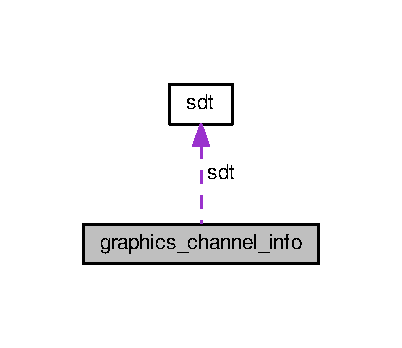
\includegraphics[width=193pt]{structgraphics__channel__info__coll__graph}
\end{center}
\end{figure}
\subsection*{Data Fields}
\begin{DoxyCompactItemize}
\item 
uint16\+\_\+t \hyperlink{structgraphics__channel__info_afb009f98970631fb6229fb4264438956}{ch\+\_\+num}\hypertarget{structgraphics__channel__info_afb009f98970631fb6229fb4264438956}{}\label{structgraphics__channel__info_afb009f98970631fb6229fb4264438956}

\begin{DoxyCompactList}\small\item\em The number of the channel. \end{DoxyCompactList}\item 
bool \hyperlink{structgraphics__channel__info_ac899174418a5cd8b4f7fd4948d5f590c}{teletext}\hypertarget{structgraphics__channel__info_ac899174418a5cd8b4f7fd4948d5f590c}{}\label{structgraphics__channel__info_ac899174418a5cd8b4f7fd4948d5f590c}

\begin{DoxyCompactList}\small\item\em Whether the channel has teletext. \end{DoxyCompactList}\item 
uint16\+\_\+t \hyperlink{structgraphics__channel__info_a3cf334be574a33699fef2f2ee28aa6a8}{vpid}\hypertarget{structgraphics__channel__info_a3cf334be574a33699fef2f2ee28aa6a8}{}\label{structgraphics__channel__info_a3cf334be574a33699fef2f2ee28aa6a8}

\begin{DoxyCompactList}\small\item\em The video P\+ID of the channel. \end{DoxyCompactList}\item 
uint16\+\_\+t \hyperlink{structgraphics__channel__info_a4518e8c7dccf92ed956ff9a517520ee1}{apid}\hypertarget{structgraphics__channel__info_a4518e8c7dccf92ed956ff9a517520ee1}{}\label{structgraphics__channel__info_a4518e8c7dccf92ed956ff9a517520ee1}

\begin{DoxyCompactList}\small\item\em The audio P\+ID of the channel. \end{DoxyCompactList}\item 
struct \hyperlink{structsdt}{sdt} \hyperlink{structgraphics__channel__info_a290b1f3b5219b69165e6b7bde53d9c37}{sdt}\hypertarget{structgraphics__channel__info_a290b1f3b5219b69165e6b7bde53d9c37}{}\label{structgraphics__channel__info_a290b1f3b5219b69165e6b7bde53d9c37}

\begin{DoxyCompactList}\small\item\em Channel type and name. \end{DoxyCompactList}\item 
struct tm \hyperlink{structgraphics__channel__info_a6acd02cb8ba22b89c8f39caca2b69620}{tm}\hypertarget{structgraphics__channel__info_a6acd02cb8ba22b89c8f39caca2b69620}{}\label{structgraphics__channel__info_a6acd02cb8ba22b89c8f39caca2b69620}

\begin{DoxyCompactList}\small\item\em Time information. \end{DoxyCompactList}\end{DoxyCompactItemize}


\subsection{Detailed Description}
A struct that contains some basic channel info. 

The documentation for this struct was generated from the following file\+:\begin{DoxyCompactItemize}
\item 
include/\hyperlink{graphics_8h}{graphics.\+h}\end{DoxyCompactItemize}

\hypertarget{structgraphics__flags}{}\section{graphics\+\_\+flags Struct Reference}
\label{structgraphics__flags}\index{graphics\+\_\+flags@{graphics\+\_\+flags}}


A struct that keeps the state of what should be displayed.  


\subsection*{Data Fields}
\begin{DoxyCompactItemize}
\item 
bool \hyperlink{structgraphics__flags_a8c60d4b825e87dbc322912b94395285b}{info}\hypertarget{structgraphics__flags_a8c60d4b825e87dbc322912b94395285b}{}\label{structgraphics__flags_a8c60d4b825e87dbc322912b94395285b}

\begin{DoxyCompactList}\small\item\em Specifies whether the info panel should be displayed. \end{DoxyCompactList}\item 
bool \hyperlink{structgraphics__flags_aa00a1018a3820d20a55a36da5b21e966}{volume}\hypertarget{structgraphics__flags_aa00a1018a3820d20a55a36da5b21e966}{}\label{structgraphics__flags_aa00a1018a3820d20a55a36da5b21e966}

\begin{DoxyCompactList}\small\item\em Specifies whether the volume panel should be displayed. \end{DoxyCompactList}\item 
bool \hyperlink{structgraphics__flags_a499f89ea543aef799513d071bff759b6}{blackscreen}\hypertarget{structgraphics__flags_a499f89ea543aef799513d071bff759b6}{}\label{structgraphics__flags_a499f89ea543aef799513d071bff759b6}

\begin{DoxyCompactList}\small\item\em Specifies whether the screen should be filled with black. \end{DoxyCompactList}\item 
bool \hyperlink{structgraphics__flags_afe0faa55883d9f711190fe31fa4b189f}{no\+\_\+channel}\hypertarget{structgraphics__flags_afe0faa55883d9f711190fe31fa4b189f}{}\label{structgraphics__flags_afe0faa55883d9f711190fe31fa4b189f}

\begin{DoxyCompactList}\small\item\em Specifies whether the \char`\"{}\+N\+O C\+H\+A\+N\+N\+E\+L\char`\"{} message should be displayed. \end{DoxyCompactList}\item 
bool \hyperlink{structgraphics__flags_aad6f429cd9f715a69bb14e2abf6db718}{audio\+\_\+only}\hypertarget{structgraphics__flags_aad6f429cd9f715a69bb14e2abf6db718}{}\label{structgraphics__flags_aad6f429cd9f715a69bb14e2abf6db718}

\begin{DoxyCompactList}\small\item\em Specifies whether the \char`\"{}\+A\+U\+D\+I\+O O\+N\+L\+Y\char`\"{} message should be displayed. \end{DoxyCompactList}\item 
bool \hyperlink{structgraphics__flags_a9def1d8fb73e0175f0d2a27331732f19}{ch\+\_\+num}\hypertarget{structgraphics__flags_a9def1d8fb73e0175f0d2a27331732f19}{}\label{structgraphics__flags_a9def1d8fb73e0175f0d2a27331732f19}

\begin{DoxyCompactList}\small\item\em Specifies whether the top left channel number should be displayed. \end{DoxyCompactList}\item 
bool \hyperlink{structgraphics__flags_acda6aca3d8288e5b1c0d2648957698a3}{time}\hypertarget{structgraphics__flags_acda6aca3d8288e5b1c0d2648957698a3}{}\label{structgraphics__flags_acda6aca3d8288e5b1c0d2648957698a3}

\begin{DoxyCompactList}\small\item\em Specifies whether the time should be displayed. \end{DoxyCompactList}\item 
bool \hyperlink{structgraphics__flags_a72ec7ac8b062a1a6dde4662b4af31208}{init}\hypertarget{structgraphics__flags_a72ec7ac8b062a1a6dde4662b4af31208}{}\label{structgraphics__flags_a72ec7ac8b062a1a6dde4662b4af31208}

\begin{DoxyCompactList}\small\item\em Specifies whether the \char`\"{}\+I\+N\+I\+T\+I\+A\+L\+I\+Z\+I\+N\+G\char`\"{} message should be displayed. \end{DoxyCompactList}\item 
bool \hyperlink{structgraphics__flags_a3309b3b318980c66dc349e26707f039c}{mute}\hypertarget{structgraphics__flags_a3309b3b318980c66dc349e26707f039c}{}\label{structgraphics__flags_a3309b3b318980c66dc349e26707f039c}

\begin{DoxyCompactList}\small\item\em Specifies whether the mute symbol should be displayed. Takes precedence over \hyperlink{structgraphics__flags_aa00a1018a3820d20a55a36da5b21e966}{volume}. \end{DoxyCompactList}\end{DoxyCompactItemize}


\subsection{Detailed Description}
A struct that keeps the state of what should be displayed. 

The documentation for this struct was generated from the following file\+:\begin{DoxyCompactItemize}
\item 
src/\hyperlink{graphics_8c}{graphics.\+c}\end{DoxyCompactItemize}

\hypertarget{structpat}{}\section{pat Struct Reference}
\label{structpat}\index{pat@{pat}}


Contains important info from the P\+AT table.  




{\ttfamily \#include $<$parsing.\+h$>$}



Collaboration diagram for pat\+:\nopagebreak
\begin{figure}[H]
\begin{center}
\leavevmode
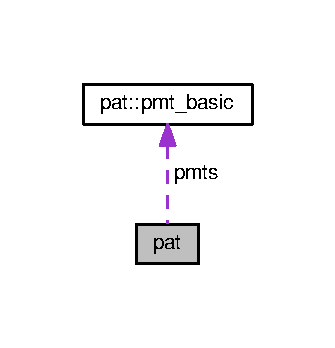
\includegraphics[width=161pt]{structpat__coll__graph}
\end{center}
\end{figure}
\subsection*{Data Structures}
\begin{DoxyCompactItemize}
\item 
struct \hyperlink{structpat_1_1pmt__basic}{pmt\+\_\+basic}
\begin{DoxyCompactList}\small\item\em Contains enough info to identify a P\+MT table. \end{DoxyCompactList}\end{DoxyCompactItemize}
\subsection*{Data Fields}
\begin{DoxyCompactItemize}
\item 
uint16\+\_\+t \hyperlink{structpat_ade45ceee5348b15b3e0d78422eff6cbe}{tsi}\hypertarget{structpat_ade45ceee5348b15b3e0d78422eff6cbe}{}\label{structpat_ade45ceee5348b15b3e0d78422eff6cbe}

\begin{DoxyCompactList}\small\item\em Transport stream id. \end{DoxyCompactList}\item 
size\+\_\+t \hyperlink{structpat_ac1d8d75f9ba19cf1dffb745fb9f41866}{pmt\+\_\+len}\hypertarget{structpat_ac1d8d75f9ba19cf1dffb745fb9f41866}{}\label{structpat_ac1d8d75f9ba19cf1dffb745fb9f41866}

\begin{DoxyCompactList}\small\item\em How many P\+M\+Ts exist in the stream. \end{DoxyCompactList}\item 
struct \hyperlink{structpat_1_1pmt__basic}{pat\+::pmt\+\_\+basic} $\ast$ \hyperlink{structpat_a6dd8e2cd3063bdb1e20711aefb88983e}{pmts}\hypertarget{structpat_a6dd8e2cd3063bdb1e20711aefb88983e}{}\label{structpat_a6dd8e2cd3063bdb1e20711aefb88983e}

\begin{DoxyCompactList}\small\item\em Array of P\+M\+Ts that exist in the stream. \end{DoxyCompactList}\end{DoxyCompactItemize}


\subsection{Detailed Description}
Contains important info from the P\+AT table. 

The documentation for this struct was generated from the following file\+:\begin{DoxyCompactItemize}
\item 
include/\hyperlink{parsing_8h}{parsing.\+h}\end{DoxyCompactItemize}

\hypertarget{structpat__body}{}\section{pat\+\_\+body Struct Reference}
\label{structpat__body}\index{pat\+\_\+body@{pat\+\_\+body}}


Represents P\+AT body.  




{\ttfamily \#include $<$structures.\+h$>$}

\subsection*{Data Fields}
\begin{DoxyCompactItemize}
\item 
uint16\+\_\+t \hyperlink{structpat__body_a598606f66a60d2c844b39a335f2ae568}{ch\+\_\+num}\hypertarget{structpat__body_a598606f66a60d2c844b39a335f2ae568}{}\label{structpat__body_a598606f66a60d2c844b39a335f2ae568}

\begin{DoxyCompactList}\small\item\em Channel number of the current P\+MT. \end{DoxyCompactList}\item 
\begin{tabbing}
xx\=xx\=xx\=xx\=xx\=xx\=xx\=xx\=xx\=\kill
union \{\\
\>struct \{\\
\>\>uint16\_t \hyperlink{structpat__body_ac6a89b300683b8445324a9609ce01c3d}{pid}: 13\\
\>\>\>{\em PID of the PMT table. }\\
\>\>uint16\_t {\bfseries res}: 3\\
\>\} {\bfseries b1s}\\
\>uint16\_t {\bfseries bitfield1}\\
\} {\bfseries b1u}\hypertarget{structpat__body_a8f3a02c9dcdbc8c2943c2138a5db6d5f}{}\label{structpat__body_a8f3a02c9dcdbc8c2943c2138a5db6d5f}
\\

\end{tabbing}\end{DoxyCompactItemize}


\subsection{Detailed Description}
Represents P\+AT body. 

The documentation for this struct was generated from the following file\+:\begin{DoxyCompactItemize}
\item 
include/\hyperlink{structures_8h}{structures.\+h}\end{DoxyCompactItemize}

\hypertarget{structpat__header}{}\section{pat\+\_\+header Struct Reference}
\label{structpat__header}\index{pat\+\_\+header@{pat\+\_\+header}}


Represents P\+AT header.  




{\ttfamily \#include $<$structures.\+h$>$}



Collaboration diagram for pat\+\_\+header\+:\nopagebreak
\begin{figure}[H]
\begin{center}
\leavevmode
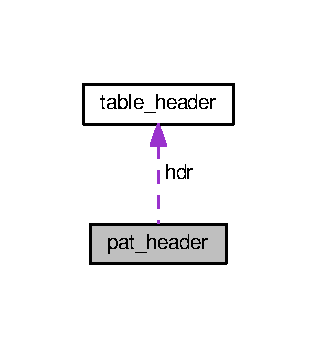
\includegraphics[width=152pt]{structpat__header__coll__graph}
\end{center}
\end{figure}
\subsection*{Data Fields}
\begin{DoxyCompactItemize}
\item 
struct \hyperlink{structtable__header}{table\+\_\+header} {\bfseries hdr}\hypertarget{structpat__header_aba3506df2bd57dfea7f4eda3b31923e1}{}\label{structpat__header_aba3506df2bd57dfea7f4eda3b31923e1}

\item 
uint16\+\_\+t {\bfseries tsi}\hypertarget{structpat__header_ae911aee2f0283dfb8d45945f403a6456}{}\label{structpat__header_ae911aee2f0283dfb8d45945f403a6456}

\item 
\begin{tabbing}
xx\=xx\=xx\=xx\=xx\=xx\=xx\=xx\=xx\=\kill
struct \{\\
\>uint8\_t {\bfseries cni}: 1\\
\>uint8\_t {\bfseries version}: 5\\
\>uint8\_t {\bfseries res}: 2\\
\} {\bfseries b1s}\hypertarget{structpat__header_a212fe9c2d650280b55695b6887a87817}{}\label{structpat__header_a212fe9c2d650280b55695b6887a87817}
\\

\end{tabbing}\item 
uint8\+\_\+t {\bfseries sec}\hypertarget{structpat__header_a0bc5a3faf64ae3afcfcee271301e73f4}{}\label{structpat__header_a0bc5a3faf64ae3afcfcee271301e73f4}

\item 
uint8\+\_\+t {\bfseries lsn}\hypertarget{structpat__header_a22345d9afb7a903eab57e516128c1505}{}\label{structpat__header_a22345d9afb7a903eab57e516128c1505}

\end{DoxyCompactItemize}


\subsection{Detailed Description}
Represents P\+AT header. 

The documentation for this struct was generated from the following file\+:\begin{DoxyCompactItemize}
\item 
include/\hyperlink{structures_8h}{structures.\+h}\end{DoxyCompactItemize}

\hypertarget{structpmt}{}\section{pmt Struct Reference}
\label{structpmt}\index{pmt@{pmt}}


Contains important info from the P\+MT table.  




{\ttfamily \#include $<$parsing.\+h$>$}

\subsection*{Data Fields}
\begin{DoxyCompactItemize}
\item 
uint16\+\_\+t \hyperlink{structpmt_a94da4c86fc671f2e2ca0b3197291c999}{pid}\hypertarget{structpmt_a94da4c86fc671f2e2ca0b3197291c999}{}\label{structpmt_a94da4c86fc671f2e2ca0b3197291c999}

\begin{DoxyCompactList}\small\item\em The pid of the P\+MT table. \end{DoxyCompactList}\item 
uint16\+\_\+t \hyperlink{structpmt_a32019497634c4f6e6b842d79f3417187}{ch\+\_\+num}\hypertarget{structpmt_a32019497634c4f6e6b842d79f3417187}{}\label{structpmt_a32019497634c4f6e6b842d79f3417187}

\begin{DoxyCompactList}\small\item\em The channel number of the P\+MT table. \end{DoxyCompactList}\item 
uint16\+\_\+t \hyperlink{structpmt_a49cc267d734db2def0cd6af31fdc60a8}{video\+\_\+pid}\hypertarget{structpmt_a49cc267d734db2def0cd6af31fdc60a8}{}\label{structpmt_a49cc267d734db2def0cd6af31fdc60a8}

\begin{DoxyCompactList}\small\item\em P\+ID of the video stream. It is -\/1 if it doesn\textquotesingle{}t exist. \end{DoxyCompactList}\item 
uint16\+\_\+t \hyperlink{structpmt_a68081a602490e42492431056f72efbd7}{audio\+\_\+pid}\hypertarget{structpmt_a68081a602490e42492431056f72efbd7}{}\label{structpmt_a68081a602490e42492431056f72efbd7}

\begin{DoxyCompactList}\small\item\em P\+ID of the audio stream. It is -\/1 if it doesn\textquotesingle{}t exist. \end{DoxyCompactList}\item 
bool \hyperlink{structpmt_ad1ddfb7a259bcc79f882418f46225e2e}{teletext}\hypertarget{structpmt_ad1ddfb7a259bcc79f882418f46225e2e}{}\label{structpmt_ad1ddfb7a259bcc79f882418f46225e2e}

\begin{DoxyCompactList}\small\item\em Specifies whether the channel has teletext. \end{DoxyCompactList}\end{DoxyCompactItemize}


\subsection{Detailed Description}
Contains important info from the P\+MT table. 

The documentation for this struct was generated from the following file\+:\begin{DoxyCompactItemize}
\item 
include/\hyperlink{parsing_8h}{parsing.\+h}\end{DoxyCompactItemize}

\hypertarget{structpat_1_1pmt__basic}{}\section{pat\+:\+:pmt\+\_\+basic Struct Reference}
\label{structpat_1_1pmt__basic}\index{pat\+::pmt\+\_\+basic@{pat\+::pmt\+\_\+basic}}


Contains enough info to identify a P\+MT table.  




{\ttfamily \#include $<$parsing.\+h$>$}

\subsection*{Data Fields}
\begin{DoxyCompactItemize}
\item 
uint16\+\_\+t \hyperlink{structpat_1_1pmt__basic_ad9371c0424eaba7e28b0867ff4ee20cb}{pid}\hypertarget{structpat_1_1pmt__basic_ad9371c0424eaba7e28b0867ff4ee20cb}{}\label{structpat_1_1pmt__basic_ad9371c0424eaba7e28b0867ff4ee20cb}

\begin{DoxyCompactList}\small\item\em The P\+ID of the P\+MT table. \end{DoxyCompactList}\item 
uint16\+\_\+t \hyperlink{structpat_1_1pmt__basic_ab0c03378d12bd321942c8a68721bcb51}{ch\+\_\+num}\hypertarget{structpat_1_1pmt__basic_ab0c03378d12bd321942c8a68721bcb51}{}\label{structpat_1_1pmt__basic_ab0c03378d12bd321942c8a68721bcb51}

\begin{DoxyCompactList}\small\item\em The channel number of the P\+MT table. \end{DoxyCompactList}\end{DoxyCompactItemize}


\subsection{Detailed Description}
Contains enough info to identify a P\+MT table. 

The documentation for this struct was generated from the following file\+:\begin{DoxyCompactItemize}
\item 
include/\hyperlink{parsing_8h}{parsing.\+h}\end{DoxyCompactItemize}

\hypertarget{structpmt__body}{}\section{pmt\+\_\+body Struct Reference}
\label{structpmt__body}\index{pmt\+\_\+body@{pmt\+\_\+body}}


Represents P\+MT body.  




{\ttfamily \#include $<$structures.\+h$>$}

\subsection*{Data Fields}
\begin{DoxyCompactItemize}
\item 
uint8\+\_\+t \hyperlink{structpmt__body_aeee07b891d89313dbe5c01b2d524bbfd}{type}\hypertarget{structpmt__body_aeee07b891d89313dbe5c01b2d524bbfd}{}\label{structpmt__body_aeee07b891d89313dbe5c01b2d524bbfd}

\begin{DoxyCompactList}\small\item\em Type of stream. \end{DoxyCompactList}\item 
\begin{tabbing}
xx\=xx\=xx\=xx\=xx\=xx\=xx\=xx\=xx\=\kill
union \{\\
\>struct \{\\
\>\>uint16\_t \hyperlink{structpmt__body_a2ef568b533b7dc10584970ee0cf79721}{pid}: 13\\
\>\>\>{\em PID of the PS. }\\
\>\>uint16\_t {\bfseries res}: 3\\
\>\} {\bfseries b1s}\\
\>uint16\_t {\bfseries bitfield1}\\
\} {\bfseries b1u}\hypertarget{structpmt__body_a0119098b67b48f3f69728abb2f019dd8}{}\label{structpmt__body_a0119098b67b48f3f69728abb2f019dd8}
\\

\end{tabbing}\item 
\begin{tabbing}
xx\=xx\=xx\=xx\=xx\=xx\=xx\=xx\=xx\=\kill
union \{\\
\>struct \{\\
\>\>uint16\_t \hyperlink{structpmt__body_a1aed7248ad83715d38b55de7c9834bf6}{esilen}: 12\\
\>\>\>{\em Length of the descriptor section. }\\
\>\>uint16\_t {\bfseries res2}: 4\\
\>\} {\bfseries b2s}\\
\>uint16\_t {\bfseries bitfield2}\\
\} {\bfseries b2u}\hypertarget{structpmt__body_a1c7aac0682666c6af7df2622b5bcbb34}{}\label{structpmt__body_a1c7aac0682666c6af7df2622b5bcbb34}
\\

\end{tabbing}\end{DoxyCompactItemize}


\subsection{Detailed Description}
Represents P\+MT body. 

The documentation for this struct was generated from the following file\+:\begin{DoxyCompactItemize}
\item 
include/\hyperlink{structures_8h}{structures.\+h}\end{DoxyCompactItemize}

\hypertarget{structpmt__header}{}\section{pmt\+\_\+header Struct Reference}
\label{structpmt__header}\index{pmt\+\_\+header@{pmt\+\_\+header}}


Represents P\+MT header.  




{\ttfamily \#include $<$structures.\+h$>$}



Collaboration diagram for pmt\+\_\+header\+:\nopagebreak
\begin{figure}[H]
\begin{center}
\leavevmode
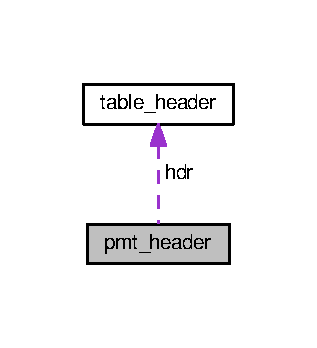
\includegraphics[width=152pt]{structpmt__header__coll__graph}
\end{center}
\end{figure}
\subsection*{Data Fields}
\begin{DoxyCompactItemize}
\item 
struct \hyperlink{structtable__header}{table\+\_\+header} {\bfseries hdr}\hypertarget{structpmt__header_a4465cd3a99485194d350b7b09c53a2cd}{}\label{structpmt__header_a4465cd3a99485194d350b7b09c53a2cd}

\item 
uint16\+\_\+t \hyperlink{structpmt__header_a24dc7745cd87ad20cb408dd2969d63bf}{ch\+\_\+num}\hypertarget{structpmt__header_a24dc7745cd87ad20cb408dd2969d63bf}{}\label{structpmt__header_a24dc7745cd87ad20cb408dd2969d63bf}

\begin{DoxyCompactList}\small\item\em Channel number. \end{DoxyCompactList}\item 
\begin{tabbing}
xx\=xx\=xx\=xx\=xx\=xx\=xx\=xx\=xx\=\kill
struct \{\\
\>uint8\_t {\bfseries cni}: 1\\
\>uint8\_t {\bfseries version}: 5\\
\>uint8\_t {\bfseries res}: 2\\
\} {\bfseries b}\hypertarget{structpmt__header_ad208096cf9e2655c5a164a9a125c7628}{}\label{structpmt__header_ad208096cf9e2655c5a164a9a125c7628}
\\

\end{tabbing}\item 
uint8\+\_\+t {\bfseries sec}\hypertarget{structpmt__header_a03530eddceb04a019b9be2edb8ea242b}{}\label{structpmt__header_a03530eddceb04a019b9be2edb8ea242b}

\item 
uint8\+\_\+t {\bfseries lsn}\hypertarget{structpmt__header_a035caa954eccf721aee42eddaa823d85}{}\label{structpmt__header_a035caa954eccf721aee42eddaa823d85}

\item 
\begin{tabbing}
xx\=xx\=xx\=xx\=xx\=xx\=xx\=xx\=xx\=\kill
union \{\\
\>struct \{\\
\>\>uint16\_t {\bfseries pcr\_pid}: 13\\
\>\>uint16\_t {\bfseries res2}: 3\\
\>\} {\bfseries b1s}\\
\>uint16\_t {\bfseries bitfield1}\\
\} {\bfseries b1u}\hypertarget{structpmt__header_a6b90ad8cfb7ae94d769c1dcd589f4f4f}{}\label{structpmt__header_a6b90ad8cfb7ae94d769c1dcd589f4f4f}
\\

\end{tabbing}\item 
\begin{tabbing}
xx\=xx\=xx\=xx\=xx\=xx\=xx\=xx\=xx\=\kill
union \{\\
\>struct \{\\
\>\>uint16\_t \hyperlink{structpmt__header_a365f4b386853bdd2f96459a36acf90b0}{pilen}: 12\\
\>\>\>{\em Length of the \hyperlink{structpmt__body}{pmt\_body} section. }\\
\>\>uint16\_t {\bfseries res3}: 4\\
\>\} {\bfseries b2s}\\
\>uint16\_t {\bfseries bitfield2}\\
\} {\bfseries b2u}\hypertarget{structpmt__header_a1be8b71e69b4723855acc265732a87a3}{}\label{structpmt__header_a1be8b71e69b4723855acc265732a87a3}
\\

\end{tabbing}\end{DoxyCompactItemize}


\subsection{Detailed Description}
Represents P\+MT header. 

The documentation for this struct was generated from the following file\+:\begin{DoxyCompactItemize}
\item 
include/\hyperlink{structures_8h}{structures.\+h}\end{DoxyCompactItemize}

\hypertarget{structrc__args}{}\section{rc\+\_\+args Struct Reference}
\label{structrc__args}\index{rc\+\_\+args@{rc\+\_\+args}}


A shim structure to pass arguments to event thread.  


\subsection*{Data Fields}
\begin{DoxyCompactItemize}
\item 
int {\bfseries fd}\hypertarget{structrc__args_a0087985aae37c3acb4659f367022330a}{}\label{structrc__args_a0087985aae37c3acb4659f367022330a}

\item 
\hyperlink{group__rc_gaa7ca8d3e24ef0c270366ce6fd9bcd258}{rc\+\_\+key\+\_\+callback} {\bfseries kc}\hypertarget{structrc__args_af2a48ba3c9889e4e1cec2527ce56e974}{}\label{structrc__args_af2a48ba3c9889e4e1cec2527ce56e974}

\end{DoxyCompactItemize}


\subsection{Detailed Description}
A shim structure to pass arguments to event thread. 

The documentation for this struct was generated from the following file\+:\begin{DoxyCompactItemize}
\item 
src/\hyperlink{rc_8c}{rc.\+c}\end{DoxyCompactItemize}

\hypertarget{structsdt}{}\section{sdt Struct Reference}
\label{structsdt}\index{sdt@{sdt}}


Contains important info from the S\+DT table.  




{\ttfamily \#include $<$parsing.\+h$>$}

\subsection*{Data Fields}
\begin{DoxyCompactItemize}
\item 
uint8\+\_\+t \hyperlink{structsdt_a8c814c6244e0242de75f1dbde51aed17}{st}\hypertarget{structsdt_a8c814c6244e0242de75f1dbde51aed17}{}\label{structsdt_a8c814c6244e0242de75f1dbde51aed17}

\begin{DoxyCompactList}\small\item\em Service type. \end{DoxyCompactList}\item 
char \hyperlink{structsdt_a2339e7ee708d4fedf48653d8fae39ab7}{name} \mbox{[}100\mbox{]}\hypertarget{structsdt_a2339e7ee708d4fedf48653d8fae39ab7}{}\label{structsdt_a2339e7ee708d4fedf48653d8fae39ab7}

\begin{DoxyCompactList}\small\item\em Channel name. \end{DoxyCompactList}\end{DoxyCompactItemize}


\subsection{Detailed Description}
Contains important info from the S\+DT table. 

The documentation for this struct was generated from the following file\+:\begin{DoxyCompactItemize}
\item 
include/\hyperlink{parsing_8h}{parsing.\+h}\end{DoxyCompactItemize}

\hypertarget{structsdt__body}{}\section{sdt\+\_\+body Struct Reference}
\label{structsdt__body}\index{sdt\+\_\+body@{sdt\+\_\+body}}


Represents S\+DT body.  




{\ttfamily \#include $<$structures.\+h$>$}

\subsection*{Data Fields}
\begin{DoxyCompactItemize}
\item 
uint16\+\_\+t \hyperlink{structsdt__body_afcbfe244b8b3ac5ce90476403d80b942}{sid}\hypertarget{structsdt__body_afcbfe244b8b3ac5ce90476403d80b942}{}\label{structsdt__body_afcbfe244b8b3ac5ce90476403d80b942}

\begin{DoxyCompactList}\small\item\em Service id (same as channel number). \end{DoxyCompactList}\item 
\begin{tabbing}
xx\=xx\=xx\=xx\=xx\=xx\=xx\=xx\=xx\=\kill
struct \{\\
\>uint8\_t {\bfseries epff}: 1\\
\>uint8\_t {\bfseries esf}: 1\\
\>uint8\_t {\bfseries res}: 6\\
\} {\bfseries b1s}\hypertarget{structsdt__body_a2a62cac7031e11b79a4e8901126f5abe}{}\label{structsdt__body_a2a62cac7031e11b79a4e8901126f5abe}
\\

\end{tabbing}\item 
\begin{tabbing}
xx\=xx\=xx\=xx\=xx\=xx\=xx\=xx\=xx\=\kill
union \{\\
\>struct \{\\
\>\>uint16\_t \hyperlink{structsdt__body_a228e2b0e07a2989524f454aec4f005a6}{dlen}: 12\\
\>\>\>{\em Length of the descriptor section. }\\
\>\>uint16\_t {\bfseries fcm}: 1\\
\>\>uint16\_t {\bfseries rs}: 3\\
\>\} {\bfseries b2s}\\
\>uint16\_t {\bfseries bitfield2}\\
\} {\bfseries b2u}\hypertarget{structsdt__body_a9cb497af4c7fdd9f47d0120b08404faa}{}\label{structsdt__body_a9cb497af4c7fdd9f47d0120b08404faa}
\\

\end{tabbing}\end{DoxyCompactItemize}


\subsection{Detailed Description}
Represents S\+DT body. 

The documentation for this struct was generated from the following file\+:\begin{DoxyCompactItemize}
\item 
include/\hyperlink{structures_8h}{structures.\+h}\end{DoxyCompactItemize}

\hypertarget{structsdt__descriptor1}{}\section{sdt\+\_\+descriptor1 Struct Reference}
\label{structsdt__descriptor1}\index{sdt\+\_\+descriptor1@{sdt\+\_\+descriptor1}}


Represents the first half of the service descriptor.  




{\ttfamily \#include $<$structures.\+h$>$}

\subsection*{Data Fields}
\begin{DoxyCompactItemize}
\item 
uint8\+\_\+t {\bfseries tag}\hypertarget{structsdt__descriptor1_aa016fa383d1adbba32c10213d468da56}{}\label{structsdt__descriptor1_aa016fa383d1adbba32c10213d468da56}

\item 
uint8\+\_\+t \hyperlink{structsdt__descriptor1_a8ae0d9f33bf71c2246a31282ea9a3dad}{len}\hypertarget{structsdt__descriptor1_a8ae0d9f33bf71c2246a31282ea9a3dad}{}\label{structsdt__descriptor1_a8ae0d9f33bf71c2246a31282ea9a3dad}

\begin{DoxyCompactList}\small\item\em Length of the descriptor. \end{DoxyCompactList}\item 
uint8\+\_\+t \hyperlink{structsdt__descriptor1_a3b97c6652a50982dd0224a8abde26c0f}{type}\hypertarget{structsdt__descriptor1_a3b97c6652a50982dd0224a8abde26c0f}{}\label{structsdt__descriptor1_a3b97c6652a50982dd0224a8abde26c0f}

\begin{DoxyCompactList}\small\item\em Type of service (channel). \end{DoxyCompactList}\item 
uint8\+\_\+t \hyperlink{structsdt__descriptor1_aad8404a3a38becdc9bf617787824c328}{spnlen}\hypertarget{structsdt__descriptor1_aad8404a3a38becdc9bf617787824c328}{}\label{structsdt__descriptor1_aad8404a3a38becdc9bf617787824c328}

\begin{DoxyCompactList}\small\item\em Length of the service provider name. \end{DoxyCompactList}\end{DoxyCompactItemize}


\subsection{Detailed Description}
Represents the first half of the service descriptor. 

The documentation for this struct was generated from the following file\+:\begin{DoxyCompactItemize}
\item 
include/\hyperlink{structures_8h}{structures.\+h}\end{DoxyCompactItemize}

\hypertarget{structsdt__descriptor2}{}\section{sdt\+\_\+descriptor2 Struct Reference}
\label{structsdt__descriptor2}\index{sdt\+\_\+descriptor2@{sdt\+\_\+descriptor2}}


Represents the second half of the service descriptor.  




{\ttfamily \#include $<$structures.\+h$>$}

\subsection*{Data Fields}
\begin{DoxyCompactItemize}
\item 
uint8\+\_\+t \hyperlink{structsdt__descriptor2_a8c87b53d35ef2ea21a8bce6e99eaa740}{snlen}\hypertarget{structsdt__descriptor2_a8c87b53d35ef2ea21a8bce6e99eaa740}{}\label{structsdt__descriptor2_a8c87b53d35ef2ea21a8bce6e99eaa740}

\begin{DoxyCompactList}\small\item\em Length of the service name. \end{DoxyCompactList}\end{DoxyCompactItemize}


\subsection{Detailed Description}
Represents the second half of the service descriptor. 

The documentation for this struct was generated from the following file\+:\begin{DoxyCompactItemize}
\item 
include/\hyperlink{structures_8h}{structures.\+h}\end{DoxyCompactItemize}

\hypertarget{structsdt__header}{}\section{sdt\+\_\+header Struct Reference}
\label{structsdt__header}\index{sdt\+\_\+header@{sdt\+\_\+header}}


Represents S\+DT header.  




{\ttfamily \#include $<$structures.\+h$>$}



Collaboration diagram for sdt\+\_\+header\+:\nopagebreak
\begin{figure}[H]
\begin{center}
\leavevmode
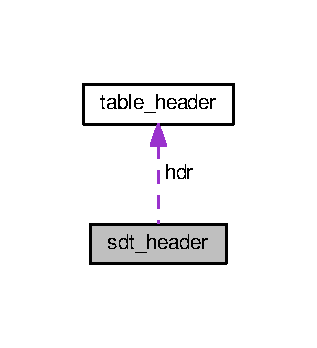
\includegraphics[width=152pt]{structsdt__header__coll__graph}
\end{center}
\end{figure}
\subsection*{Data Fields}
\begin{DoxyCompactItemize}
\item 
struct \hyperlink{structtable__header}{table\+\_\+header} {\bfseries hdr}\hypertarget{structsdt__header_a76653d315da95437fbe376d846417a95}{}\label{structsdt__header_a76653d315da95437fbe376d846417a95}

\item 
uint16\+\_\+t {\bfseries tsi}\hypertarget{structsdt__header_a38146283605f14f7ba1fb3ade2c9553e}{}\label{structsdt__header_a38146283605f14f7ba1fb3ade2c9553e}

\item 
\begin{tabbing}
xx\=xx\=xx\=xx\=xx\=xx\=xx\=xx\=xx\=\kill
struct \{\\
\>uint8\_t {\bfseries cni}: 1\\
\>uint8\_t {\bfseries version}: 5\\
\>uint8\_t {\bfseries res}: 2\\
\} {\bfseries b1s}\hypertarget{structsdt__header_a625ba58abca543c0fe8513672258eee0}{}\label{structsdt__header_a625ba58abca543c0fe8513672258eee0}
\\

\end{tabbing}\item 
uint8\+\_\+t {\bfseries sec}\hypertarget{structsdt__header_a660008af823b9b1a74b36315f799fc57}{}\label{structsdt__header_a660008af823b9b1a74b36315f799fc57}

\item 
uint8\+\_\+t {\bfseries lsn}\hypertarget{structsdt__header_a4aeb8ddd115df57e9730ed548bd83ab2}{}\label{structsdt__header_a4aeb8ddd115df57e9730ed548bd83ab2}

\item 
uint16\+\_\+t {\bfseries oni}\hypertarget{structsdt__header_af3410c6d0eafc0c8aed7596323ea4293}{}\label{structsdt__header_af3410c6d0eafc0c8aed7596323ea4293}

\item 
uint8\+\_\+t {\bfseries res2}\hypertarget{structsdt__header_ab183c41ae92058daf90868ffb0495486}{}\label{structsdt__header_ab183c41ae92058daf90868ffb0495486}

\end{DoxyCompactItemize}


\subsection{Detailed Description}
Represents S\+DT header. 

The documentation for this struct was generated from the following file\+:\begin{DoxyCompactItemize}
\item 
include/\hyperlink{structures_8h}{structures.\+h}\end{DoxyCompactItemize}

\hypertarget{structtable__header}{}\section{table\+\_\+header Struct Reference}
\label{structtable__header}\index{table\+\_\+header@{table\+\_\+header}}


Header that is part of all tables.  




{\ttfamily \#include $<$structures.\+h$>$}

\subsection*{Data Fields}
\begin{DoxyCompactItemize}
\item 
uint8\+\_\+t \hyperlink{structtable__header_a44f7dcd0d3d6a4f67c9cafac765274a9}{tid}\hypertarget{structtable__header_a44f7dcd0d3d6a4f67c9cafac765274a9}{}\label{structtable__header_a44f7dcd0d3d6a4f67c9cafac765274a9}

\begin{DoxyCompactList}\small\item\em Table id. \end{DoxyCompactList}\item 
\begin{tabbing}
xx\=xx\=xx\=xx\=xx\=xx\=xx\=xx\=xx\=\kill
union \{\\
\>struct \{\\
\>\>uint16\_t \hyperlink{structtable__header_a518aede5847a99d2a592f918f8011a47}{len}: 12\\
\>\>\>{\em Length of the rest of the table. }\\
\>\>uint16\_t {\bfseries res}: 2\\
\>\>uint16\_t {\bfseries zero}: 1\\
\>\>uint16\_t {\bfseries ssi}: 1\\
\>\} {\bfseries b1s}\\
\>uint16\_t {\bfseries bitfield1}\\
\} {\bfseries b1u}\hypertarget{structtable__header_adf4158f32bb426ab6831f3cc39bdd1cb}{}\label{structtable__header_adf4158f32bb426ab6831f3cc39bdd1cb}
\\

\end{tabbing}\end{DoxyCompactItemize}


\subsection{Detailed Description}
Header that is part of all tables. 

The documentation for this struct was generated from the following file\+:\begin{DoxyCompactItemize}
\item 
include/\hyperlink{structures_8h}{structures.\+h}\end{DoxyCompactItemize}

\hypertarget{structteletext__descriptor__header}{}\section{teletext\+\_\+descriptor\+\_\+header Struct Reference}
\label{structteletext__descriptor__header}\index{teletext\+\_\+descriptor\+\_\+header@{teletext\+\_\+descriptor\+\_\+header}}


Represents the teletext descriptor header.  




{\ttfamily \#include $<$structures.\+h$>$}

\subsection*{Data Fields}
\begin{DoxyCompactItemize}
\item 
uint8\+\_\+t \hyperlink{structteletext__descriptor__header_ac2b94f4990bbc8949e1d50fd666dc46d}{tag}\hypertarget{structteletext__descriptor__header_ac2b94f4990bbc8949e1d50fd666dc46d}{}\label{structteletext__descriptor__header_ac2b94f4990bbc8949e1d50fd666dc46d}

\begin{DoxyCompactList}\small\item\em Tag, should be 0x56. \end{DoxyCompactList}\item 
uint8\+\_\+t \hyperlink{structteletext__descriptor__header_a41535e9254cd6304dbb9ec6b72e0c2b4}{len}\hypertarget{structteletext__descriptor__header_a41535e9254cd6304dbb9ec6b72e0c2b4}{}\label{structteletext__descriptor__header_a41535e9254cd6304dbb9ec6b72e0c2b4}

\begin{DoxyCompactList}\small\item\em Length of the descriptor. \end{DoxyCompactList}\end{DoxyCompactItemize}


\subsection{Detailed Description}
Represents the teletext descriptor header. 

The documentation for this struct was generated from the following file\+:\begin{DoxyCompactItemize}
\item 
include/\hyperlink{structures_8h}{structures.\+h}\end{DoxyCompactItemize}

\hypertarget{structtot__descriptor__body}{}\section{tot\+\_\+descriptor\+\_\+body Struct Reference}
\label{structtot__descriptor__body}\index{tot\+\_\+descriptor\+\_\+body@{tot\+\_\+descriptor\+\_\+body}}


Represents T\+OT descriptor body.  




{\ttfamily \#include $<$structures.\+h$>$}

\subsection*{Data Fields}
\begin{DoxyCompactItemize}
\item 
\begin{tabbing}
xx\=xx\=xx\=xx\=xx\=xx\=xx\=xx\=xx\=\kill
union \{\\
\>struct \{\\
\>\>uint32\_t {\bfseries cc}: 24\\
\>\>uint32\_t {\bfseries regid}: 6\\
\>\>uint32\_t {\bfseries res}: 1\\
\>\>uint32\_t {\bfseries pol}: 1\\
\>\} {\bfseries b1s}\\
\>uint32\_t {\bfseries bitfield1}\\
\} {\bfseries b1u}\hypertarget{structtot__descriptor__body_af012c6228f1ff6630924e30b42faee13}{}\label{structtot__descriptor__body_af012c6228f1ff6630924e30b42faee13}
\\

\end{tabbing}\item 
uint16\+\_\+t \hyperlink{structtot__descriptor__body_af4dea234c9a3379b34d35824ae3bbce9}{lto}\hypertarget{structtot__descriptor__body_af4dea234c9a3379b34d35824ae3bbce9}{}\label{structtot__descriptor__body_af4dea234c9a3379b34d35824ae3bbce9}

\begin{DoxyCompactList}\small\item\em Local time offset. \end{DoxyCompactList}\item 
uint8\+\_\+t {\bfseries toc} \mbox{[}5\mbox{]}\hypertarget{structtot__descriptor__body_a8c2ccc7a68537e436b0f0d7b42317e0c}{}\label{structtot__descriptor__body_a8c2ccc7a68537e436b0f0d7b42317e0c}

\item 
uint16\+\_\+t {\bfseries nto}\hypertarget{structtot__descriptor__body_a670883199a91d2c5898d16408da0badb}{}\label{structtot__descriptor__body_a670883199a91d2c5898d16408da0badb}

\end{DoxyCompactItemize}


\subsection{Detailed Description}
Represents T\+OT descriptor body. 

The documentation for this struct was generated from the following file\+:\begin{DoxyCompactItemize}
\item 
include/\hyperlink{structures_8h}{structures.\+h}\end{DoxyCompactItemize}

\hypertarget{structtot__descriptor__header}{}\section{tot\+\_\+descriptor\+\_\+header Struct Reference}
\label{structtot__descriptor__header}\index{tot\+\_\+descriptor\+\_\+header@{tot\+\_\+descriptor\+\_\+header}}


Represents T\+OT descriptor header.  




{\ttfamily \#include $<$structures.\+h$>$}

\subsection*{Data Fields}
\begin{DoxyCompactItemize}
\item 
uint8\+\_\+t {\bfseries tag}\hypertarget{structtot__descriptor__header_a582e1a3735d0ef8297cddc97e954c935}{}\label{structtot__descriptor__header_a582e1a3735d0ef8297cddc97e954c935}

\item 
uint8\+\_\+t \hyperlink{structtot__descriptor__header_ab6a192f014bf34fa28c53a5622465526}{len}\hypertarget{structtot__descriptor__header_ab6a192f014bf34fa28c53a5622465526}{}\label{structtot__descriptor__header_ab6a192f014bf34fa28c53a5622465526}

\begin{DoxyCompactList}\small\item\em Length of the descriptor body. \end{DoxyCompactList}\end{DoxyCompactItemize}


\subsection{Detailed Description}
Represents T\+OT descriptor header. 

The documentation for this struct was generated from the following file\+:\begin{DoxyCompactItemize}
\item 
include/\hyperlink{structures_8h}{structures.\+h}\end{DoxyCompactItemize}

\hypertarget{structtot__header}{}\section{tot\+\_\+header Struct Reference}
\label{structtot__header}\index{tot\+\_\+header@{tot\+\_\+header}}


Represents T\+OT header.  




{\ttfamily \#include $<$structures.\+h$>$}



Collaboration diagram for tot\+\_\+header\+:\nopagebreak
\begin{figure}[H]
\begin{center}
\leavevmode
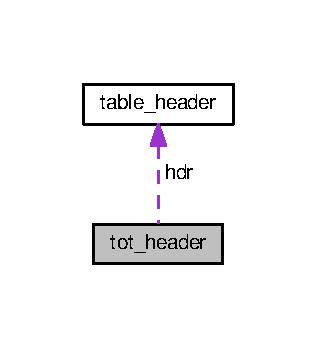
\includegraphics[width=152pt]{structtot__header__coll__graph}
\end{center}
\end{figure}
\subsection*{Data Fields}
\begin{DoxyCompactItemize}
\item 
struct \hyperlink{structtable__header}{table\+\_\+header} {\bfseries hdr}\hypertarget{structtot__header_a1c3d697481719a0e48acac326a2907b8}{}\label{structtot__header_a1c3d697481719a0e48acac326a2907b8}

\item 
uint8\+\_\+t \hyperlink{structtot__header_aca49dc8fbba34272aa461fab3540209a}{time} \mbox{[}5\mbox{]}\hypertarget{structtot__header_aca49dc8fbba34272aa461fab3540209a}{}\label{structtot__header_aca49dc8fbba34272aa461fab3540209a}

\begin{DoxyCompactList}\small\item\em Brain-\/dead encoded time information. \end{DoxyCompactList}\item 
\begin{tabbing}
xx\=xx\=xx\=xx\=xx\=xx\=xx\=xx\=xx\=\kill
union \{\\
\>struct \{\\
\>\>uint16\_t \hyperlink{structtot__header_acbbfb5cc5320d11a1f02ed41ba726540}{dlen}: 12\\
\>\>\>{\em Length of the descriptor section. }\\
\>\>uint16\_t {\bfseries res}: 4\\
\>\} {\bfseries b1s}\\
\>uint16\_t {\bfseries bitfield1}\\
\} {\bfseries b1u}\hypertarget{structtot__header_ad2cc8b0ba1378f78a2f331441003da34}{}\label{structtot__header_ad2cc8b0ba1378f78a2f331441003da34}
\\

\end{tabbing}\end{DoxyCompactItemize}


\subsection{Detailed Description}
Represents T\+OT header. 

The documentation for this struct was generated from the following file\+:\begin{DoxyCompactItemize}
\item 
include/\hyperlink{structures_8h}{structures.\+h}\end{DoxyCompactItemize}

\chapter{File Documentation}
\hypertarget{common_8h}{}\section{include/common.h File Reference}
\label{common_8h}\index{include/common.\+h@{include/common.\+h}}


Contains functions that all modules use.  


{\ttfamily \#include $<$errno.\+h$>$}\\*
{\ttfamily \#include $<$stdlib.\+h$>$}\\*
{\ttfamily \#include $<$string.\+h$>$}\\*
Include dependency graph for common.\+h\+:\nopagebreak
\begin{figure}[H]
\begin{center}
\leavevmode
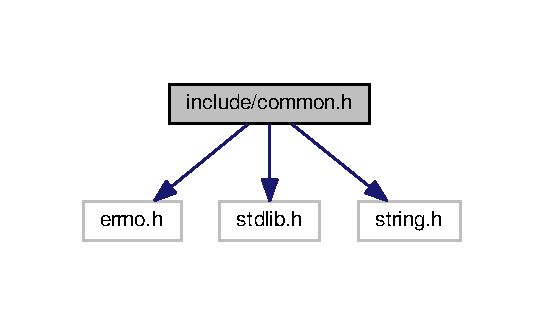
\includegraphics[width=261pt]{common_8h__incl}
\end{center}
\end{figure}
This graph shows which files directly or indirectly include this file\+:\nopagebreak
\begin{figure}[H]
\begin{center}
\leavevmode
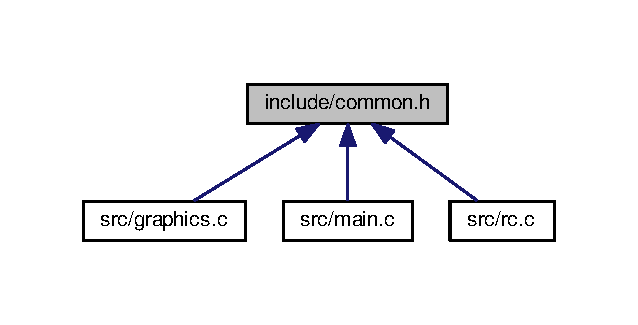
\includegraphics[width=306pt]{common_8h__dep__incl}
\end{center}
\end{figure}
\subsection*{Macros}
\begin{DoxyCompactItemize}
\item 
\#define \hyperlink{common_8h_a235bdec0a6bf62f3b3af87e528109847}{nameof}(x)~\#x\hypertarget{common_8h_a235bdec0a6bf62f3b3af87e528109847}{}\label{common_8h_a235bdec0a6bf62f3b3af87e528109847}

\begin{DoxyCompactList}\small\item\em Gets the string representation of its parameter. \end{DoxyCompactList}\item 
\#define \hyperlink{common_8h_aec09b115ba14ee07180282a0c2c87de5}{F\+A\+IL}(fmt, ...)
\begin{DoxyCompactList}\small\item\em Prints an error message to stderr and exits the program. \end{DoxyCompactList}\item 
\#define \hyperlink{common_8h_ab927a63ec0a50836c92ac3fe62a60dc3}{F\+A\+I\+L\+\_\+\+S\+TD}(fmt, ...)~\hyperlink{common_8h_aec09b115ba14ee07180282a0c2c87de5}{F\+A\+IL}(\char`\"{}\%s\+: \char`\"{}fmt, strerror(errno), \#\#\+\_\+\+\_\+\+V\+A\+\_\+\+A\+R\+G\+S\+\_\+\+\_\+)
\begin{DoxyCompactList}\small\item\em Same as \hyperlink{common_8h_aec09b115ba14ee07180282a0c2c87de5}{F\+A\+IL}, except that it also prints the string representation of errno. \end{DoxyCompactList}\item 
\#define \hyperlink{common_8h_ac464f11a32500a31842789297a3c31f4}{L\+OG}(module,  fmt, ...)
\begin{DoxyCompactList}\small\item\em Prints out a log message. \end{DoxyCompactList}\end{DoxyCompactItemize}


\subsection{Detailed Description}
Contains functions that all modules use. 



\subsection{Macro Definition Documentation}
\index{common.\+h@{common.\+h}!F\+A\+IL@{F\+A\+IL}}
\index{F\+A\+IL@{F\+A\+IL}!common.\+h@{common.\+h}}
\subsubsection[{\texorpdfstring{F\+A\+IL}{FAIL}}]{\setlength{\rightskip}{0pt plus 5cm}\#define F\+A\+IL(
\begin{DoxyParamCaption}
\item[{}]{fmt, }
\item[{}]{...}
\end{DoxyParamCaption}
)}\hypertarget{common_8h_aec09b115ba14ee07180282a0c2c87de5}{}\label{common_8h_aec09b115ba14ee07180282a0c2c87de5}
{\bfseries Value\+:}
\begin{DoxyCode}
\textcolor{keywordflow}{do} \(\backslash\)
    \{ \(\backslash\)
        fprintf(stderr, \textcolor{stringliteral}{"%s:%d:%s: Error: "}fmt, \(\backslash\)
        \_\_FILE\_\_, \_\_LINE\_\_, \_\_func\_\_, ##\_\_VA\_ARGS\_\_); \(\backslash\)
        exit(EXIT\_FAILURE); \(\backslash\)
    \} \textcolor{keywordflow}{while} (0)
\end{DoxyCode}


Prints an error message to stderr and exits the program. 


\begin{DoxyParams}{Parameters}
{\em fmt} & A printf-\/like format string. \\
\hline
{\em ...} & printf-\/like arguments to print. \\
\hline
\end{DoxyParams}
\index{common.\+h@{common.\+h}!F\+A\+I\+L\+\_\+\+S\+TD@{F\+A\+I\+L\+\_\+\+S\+TD}}
\index{F\+A\+I\+L\+\_\+\+S\+TD@{F\+A\+I\+L\+\_\+\+S\+TD}!common.\+h@{common.\+h}}
\subsubsection[{\texorpdfstring{F\+A\+I\+L\+\_\+\+S\+TD}{FAIL_STD}}]{\setlength{\rightskip}{0pt plus 5cm}\#define F\+A\+I\+L\+\_\+\+S\+TD(
\begin{DoxyParamCaption}
\item[{}]{fmt, }
\item[{}]{...}
\end{DoxyParamCaption}
)~{\bf F\+A\+IL}(\char`\"{}\%s\+: \char`\"{}fmt, strerror(errno), \#\#\+\_\+\+\_\+\+V\+A\+\_\+\+A\+R\+G\+S\+\_\+\+\_\+)}\hypertarget{common_8h_ab927a63ec0a50836c92ac3fe62a60dc3}{}\label{common_8h_ab927a63ec0a50836c92ac3fe62a60dc3}


Same as \hyperlink{common_8h_aec09b115ba14ee07180282a0c2c87de5}{F\+A\+IL}, except that it also prints the string representation of errno. 


\begin{DoxyParams}{Parameters}
{\em fmt} & A printf-\/like format string. \\
\hline
{\em ...} & printf-\/like arguments to print. \\
\hline
\end{DoxyParams}
\index{common.\+h@{common.\+h}!L\+OG@{L\+OG}}
\index{L\+OG@{L\+OG}!common.\+h@{common.\+h}}
\subsubsection[{\texorpdfstring{L\+OG}{LOG}}]{\setlength{\rightskip}{0pt plus 5cm}\#define L\+OG(
\begin{DoxyParamCaption}
\item[{}]{module, }
\item[{}]{fmt, }
\item[{}]{...}
\end{DoxyParamCaption}
)}\hypertarget{common_8h_ac464f11a32500a31842789297a3c31f4}{}\label{common_8h_ac464f11a32500a31842789297a3c31f4}
{\bfseries Value\+:}
\begin{DoxyCode}
\textcolor{keywordflow}{do} \(\backslash\)
    \{ \(\backslash\)
        printf(module\textcolor{stringliteral}{": "}fmt, ##\_\_VA\_ARGS\_\_); \(\backslash\)
    \} \textcolor{keywordflow}{while} (0)
\end{DoxyCode}


Prints out a log message. 


\begin{DoxyParams}{Parameters}
{\em module} & A string that identifies the module in which L\+OG is called. \\
\hline
{\em fmt} & A printf-\/like format string. \\
\hline
{\em ...} & printf-\/like arguments to print. \\
\hline
\end{DoxyParams}

\hypertarget{config_8h}{}\section{include/config.h File Reference}
\label{config_8h}\index{include/config.\+h@{include/config.\+h}}


Contains configuration file A\+PI.  


{\ttfamily \#include $<$stdio.\+h$>$}\\*
{\ttfamily \#include \char`\"{}tdp\+\_\+api.\+h\char`\"{}}\\*
Include dependency graph for config.\+h\+:\nopagebreak
\begin{figure}[H]
\begin{center}
\leavevmode
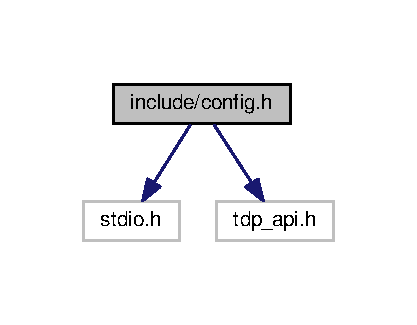
\includegraphics[width=200pt]{config_8h__incl}
\end{center}
\end{figure}
This graph shows which files directly or indirectly include this file\+:\nopagebreak
\begin{figure}[H]
\begin{center}
\leavevmode
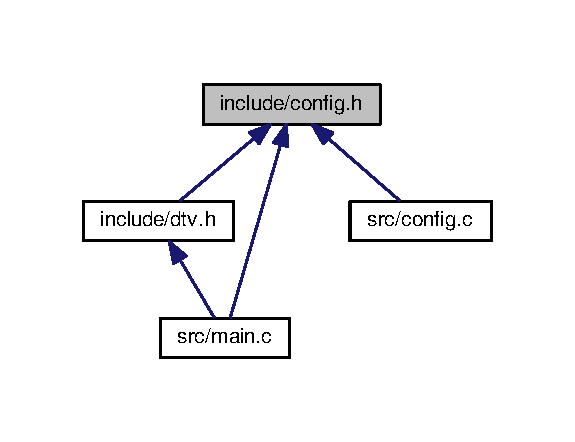
\includegraphics[width=276pt]{config_8h__dep__incl}
\end{center}
\end{figure}
\subsection*{Data Structures}
\begin{DoxyCompactItemize}
\item 
struct \hyperlink{structconfig__init__ch__info}{config\+\_\+init\+\_\+ch\+\_\+info}
\begin{DoxyCompactList}\small\item\em A structure that holds the initial dtv settings. \end{DoxyCompactList}\end{DoxyCompactItemize}
\subsection*{Functions}
\begin{DoxyCompactItemize}
\item 
struct \hyperlink{structconfig__init__ch__info}{config\+\_\+init\+\_\+ch\+\_\+info} \hyperlink{group__config_gad7d820530151b1bb2b6cf6e992f48331}{config\+\_\+get\+\_\+init\+\_\+ch\+\_\+info} (F\+I\+LE $\ast$f)
\begin{DoxyCompactList}\small\item\em Reads the initial settings from the specified file. \end{DoxyCompactList}\end{DoxyCompactItemize}


\subsection{Detailed Description}
Contains configuration file A\+PI. 


\hypertarget{drawing_8h}{}\section{include/drawing.h File Reference}
\label{drawing_8h}\index{include/drawing.\+h@{include/drawing.\+h}}


Contains A\+PI for drawing graphics elements.  


{\ttfamily \#include $<$stdint.\+h$>$}\\*
{\ttfamily \#include $<$directfb.\+h$>$}\\*
{\ttfamily \#include \char`\"{}graphics.\+h\char`\"{}}\\*
Include dependency graph for drawing.\+h\+:\nopagebreak
\begin{figure}[H]
\begin{center}
\leavevmode
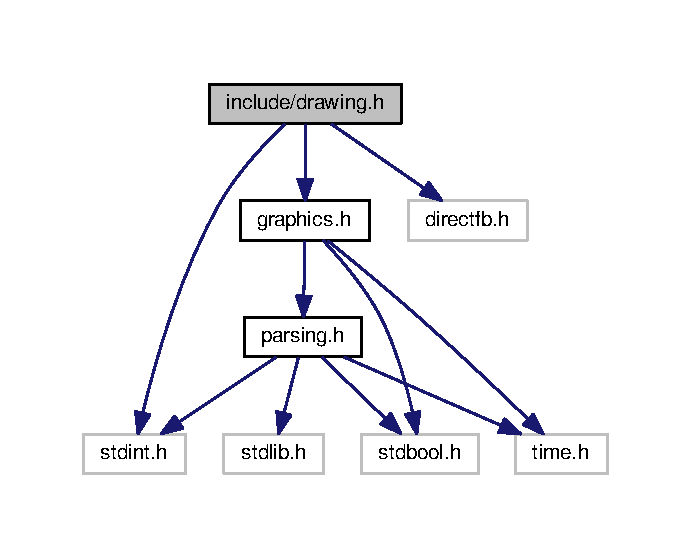
\includegraphics[width=332pt]{drawing_8h__incl}
\end{center}
\end{figure}
\subsection*{Data Structures}
\begin{DoxyCompactItemize}
\item 
struct \hyperlink{structdraw__interface}{draw\+\_\+interface}
\begin{DoxyCompactList}\small\item\em Basic interface necessary to display graphics elements. \end{DoxyCompactList}\end{DoxyCompactItemize}
\subsection*{Functions}
\begin{DoxyCompactItemize}
\item 
int32\+\_\+t \hyperlink{group__drawing_ga50526d5e4e244599996608371f410bf2}{draw\+\_\+init} (struct \hyperlink{structdraw__interface}{draw\+\_\+interface} $\ast$draw\+\_\+i, int $\ast$argc, char $\ast$$\ast$$\ast$argv)
\begin{DoxyCompactList}\small\item\em Initialize drawing interface. \end{DoxyCompactList}\item 
int32\+\_\+t \hyperlink{group__drawing_ga71818ed76471623e9aeffe07a0ba26d2}{draw\+\_\+channel\+\_\+info} (struct \hyperlink{structdraw__interface}{draw\+\_\+interface} $\ast$draw\+\_\+i, struct \hyperlink{structgraphics__channel__info}{graphics\+\_\+channel\+\_\+info} info)
\begin{DoxyCompactList}\small\item\em Draw channel\+\_\+info graphics element. \end{DoxyCompactList}\item 
int32\+\_\+t \hyperlink{group__drawing_ga37e840145ddb9107f2efbec80697e377}{draw\+\_\+init\+\_\+message} (struct \hyperlink{structdraw__interface}{draw\+\_\+interface} $\ast$draw\+\_\+i)
\begin{DoxyCompactList}\small\item\em Draw initializing message. \end{DoxyCompactList}\item 
int32\+\_\+t \hyperlink{group__drawing_gaa19821a33379a186117efe18a67bfea7}{draw\+\_\+time} (struct \hyperlink{structdraw__interface}{draw\+\_\+interface} $\ast$draw\+\_\+i, struct tm tm)
\begin{DoxyCompactList}\small\item\em Draw time graphics element. \end{DoxyCompactList}\item 
int32\+\_\+t \hyperlink{group__drawing_gae31d79c9ff070efa64603736bee4d252}{draw\+\_\+volume} (struct \hyperlink{structdraw__interface}{draw\+\_\+interface} $\ast$draw\+\_\+i, uint8\+\_\+t vol)
\begin{DoxyCompactList}\small\item\em Draw volume graphics element. \end{DoxyCompactList}\item 
int32\+\_\+t \hyperlink{group__drawing_ga9e57d07e991e2d951ad273cde5d5518a}{draw\+\_\+no\+\_\+channel} (struct \hyperlink{structdraw__interface}{draw\+\_\+interface} $\ast$draw\+\_\+i)
\begin{DoxyCompactList}\small\item\em Draw no channel display. \end{DoxyCompactList}\item 
int32\+\_\+t \hyperlink{group__drawing_ga4136711e3d32c79bf3261c2afb901b6f}{draw\+\_\+audio\+\_\+only} (struct \hyperlink{structdraw__interface}{draw\+\_\+interface} $\ast$draw\+\_\+i)
\begin{DoxyCompactList}\small\item\em Draw radio graphics. \end{DoxyCompactList}\item 
int32\+\_\+t \hyperlink{group__drawing_gab0f56761fdebd9a7bc3584a43777df94}{draw\+\_\+channel\+\_\+number} (struct \hyperlink{structdraw__interface}{draw\+\_\+interface} $\ast$draw\+\_\+i, uint16\+\_\+t \hyperlink{structures_8h_abcdde739cb26f5c6c2c0b87e83d1f421}{ch\+\_\+num})
\begin{DoxyCompactList}\small\item\em Draw channel number. \end{DoxyCompactList}\item 
int32\+\_\+t \hyperlink{group__drawing_ga07cd1d9f76609e912c17aa865cffa403}{draw\+\_\+blackscreen} (struct \hyperlink{structdraw__interface}{draw\+\_\+interface} $\ast$draw\+\_\+i)
\begin{DoxyCompactList}\small\item\em Draw a black rectangle. \end{DoxyCompactList}\item 
int32\+\_\+t \hyperlink{group__drawing_ga7e0866c8dbb4ef95d3708b7fa1a0393d}{draw\+\_\+clear} (struct \hyperlink{structdraw__interface}{draw\+\_\+interface} $\ast$draw\+\_\+i)
\begin{DoxyCompactList}\small\item\em Clear the screen. \end{DoxyCompactList}\item 
int32\+\_\+t \hyperlink{group__drawing_ga485befc089e203ec54c8b06c8e72c9f3}{draw\+\_\+refresh} (struct \hyperlink{structdraw__interface}{draw\+\_\+interface} $\ast$draw\+\_\+i)
\begin{DoxyCompactList}\small\item\em Refresh display. \end{DoxyCompactList}\item 
int32\+\_\+t \hyperlink{group__drawing_gae59904fcfa6a1ad70e82854e02e7833a}{draw\+\_\+deinit} (struct \hyperlink{structdraw__interface}{draw\+\_\+interface} $\ast$draw\+\_\+i)
\begin{DoxyCompactList}\small\item\em Deinitialize drawing interface. \end{DoxyCompactList}\end{DoxyCompactItemize}


\subsection{Detailed Description}
Contains A\+PI for drawing graphics elements. 


\hypertarget{dtv_8h}{}\section{include/dtv.h File Reference}
\label{dtv_8h}\index{include/dtv.\+h@{include/dtv.\+h}}


Contains D\+TV A\+PI.  


{\ttfamily \#include $<$inttypes.\+h$>$}\\*
{\ttfamily \#include $<$stdbool.\+h$>$}\\*
{\ttfamily \#include $<$stdint.\+h$>$}\\*
{\ttfamily \#include $<$time.\+h$>$}\\*
{\ttfamily \#include \char`\"{}config.\+h\char`\"{}}\\*
{\ttfamily \#include \char`\"{}parsing.\+h\char`\"{}}\\*
{\ttfamily \#include \char`\"{}tdp\+\_\+api.\+h\char`\"{}}\\*
Include dependency graph for dtv.\+h\+:\nopagebreak
\begin{figure}[H]
\begin{center}
\leavevmode
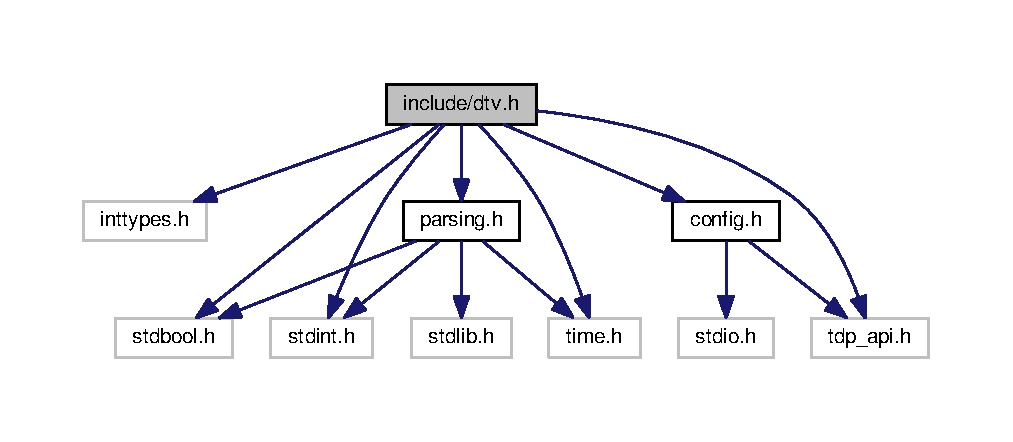
\includegraphics[width=350pt]{dtv_8h__incl}
\end{center}
\end{figure}
This graph shows which files directly or indirectly include this file\+:\nopagebreak
\begin{figure}[H]
\begin{center}
\leavevmode
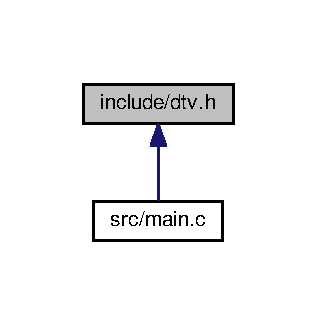
\includegraphics[width=152pt]{dtv_8h__dep__incl}
\end{center}
\end{figure}
\subsection*{Data Structures}
\begin{DoxyCompactItemize}
\item 
struct \hyperlink{structdtv__channel__info}{dtv\+\_\+channel\+\_\+info}
\begin{DoxyCompactList}\small\item\em Contains basic channel info. \end{DoxyCompactList}\end{DoxyCompactItemize}
\subsection*{Functions}
\begin{DoxyCompactItemize}
\item 
void \hyperlink{group__dtv_ga7da3a709e8d58fa00ee48687c5bf26a7}{dtv\+\_\+init} (struct \hyperlink{structconfig__init__ch__info}{config\+\_\+init\+\_\+ch\+\_\+info} init\+\_\+info)
\begin{DoxyCompactList}\small\item\em Function that initializes internal D\+TV state. \end{DoxyCompactList}\item 
struct \hyperlink{structdtv__channel__info}{dtv\+\_\+channel\+\_\+info} \hyperlink{group__dtv_gaadc265544bf474e6847f614d8a6d438e}{dtv\+\_\+switch\+\_\+channel} (uint16\+\_\+t \hyperlink{structures_8h_abcdde739cb26f5c6c2c0b87e83d1f421}{ch\+\_\+num})
\begin{DoxyCompactList}\small\item\em Tries to switch to the desired channel. \end{DoxyCompactList}\item 
t\+\_\+\+Error \hyperlink{group__dtv_gaa7f54804b10abbefca93d03afdc5aaab}{dtv\+\_\+set\+\_\+volume} (uint8\+\_\+t vol)
\begin{DoxyCompactList}\small\item\em Tries to set the volume to the desired value. \end{DoxyCompactList}\item 
struct tm \hyperlink{group__dtv_ga999f0d08fc5ddc8d4d781ccbfe10218e}{dtv\+\_\+get\+\_\+time} ()
\begin{DoxyCompactList}\small\item\em Gets the time information. \end{DoxyCompactList}\item 
struct \hyperlink{structsdt}{sdt} \hyperlink{group__dtv_ga3b7df96e66fac38b64c96e703d65e710}{dtv\+\_\+get\+\_\+info} (uint16\+\_\+t \hyperlink{structures_8h_abcdde739cb26f5c6c2c0b87e83d1f421}{ch\+\_\+num})
\begin{DoxyCompactList}\small\item\em Gets the S\+DT information for the specified channel. \end{DoxyCompactList}\item 
void \hyperlink{group__dtv_ga9d48e779ec2fdad4693156fe8923fe7b}{dtv\+\_\+deinit} ()
\begin{DoxyCompactList}\small\item\em Deinitializes the internal D\+TV state. \end{DoxyCompactList}\end{DoxyCompactItemize}


\subsection{Detailed Description}
Contains D\+TV A\+PI. 


\hypertarget{graphics_8h}{}\section{include/graphics.h File Reference}
\label{graphics_8h}\index{include/graphics.\+h@{include/graphics.\+h}}


Contains the graphics A\+PI.  


{\ttfamily \#include $<$stdbool.\+h$>$}\\*
{\ttfamily \#include $<$time.\+h$>$}\\*
{\ttfamily \#include \char`\"{}parsing.\+h\char`\"{}}\\*
Include dependency graph for graphics.\+h\+:\nopagebreak
\begin{figure}[H]
\begin{center}
\leavevmode
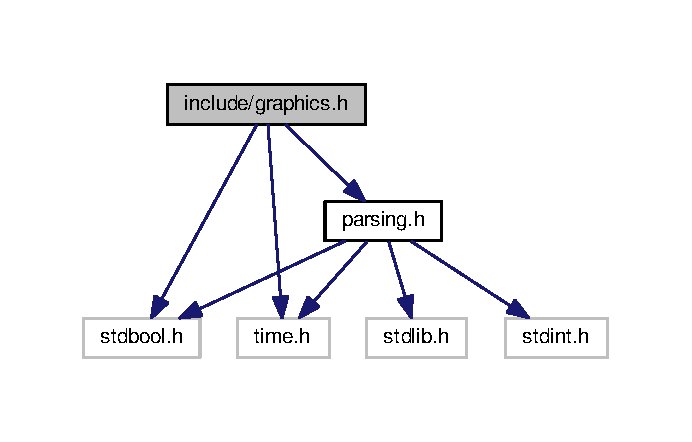
\includegraphics[width=332pt]{graphics_8h__incl}
\end{center}
\end{figure}
This graph shows which files directly or indirectly include this file\+:\nopagebreak
\begin{figure}[H]
\begin{center}
\leavevmode
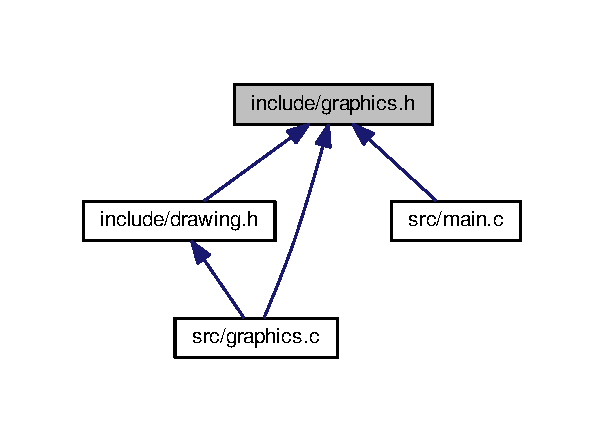
\includegraphics[width=290pt]{graphics_8h__dep__incl}
\end{center}
\end{figure}
\subsection*{Data Structures}
\begin{DoxyCompactItemize}
\item 
struct \hyperlink{structgraphics__channel__info}{graphics\+\_\+channel\+\_\+info}
\begin{DoxyCompactList}\small\item\em A struct that contains some basic channel info. \end{DoxyCompactList}\end{DoxyCompactItemize}
\subsection*{Functions}
\begin{DoxyCompactItemize}
\item 
void \hyperlink{group__graphics_ga741d634a2444a13cc83411c4bb98d948}{graphics\+\_\+show\+\_\+channel\+\_\+info} (struct \hyperlink{structgraphics__channel__info}{graphics\+\_\+channel\+\_\+info} info)
\begin{DoxyCompactList}\small\item\em Displays some basic information about a channel on the screen. \end{DoxyCompactList}\item 
void \hyperlink{group__graphics_ga07d069f854ed989682f48d8eb2b96392}{graphics\+\_\+show\+\_\+init} ()
\begin{DoxyCompactList}\small\item\em Displays initializing message. \end{DoxyCompactList}\item 
void \hyperlink{group__graphics_gaa14c15905aaa8584ac0d41629e63179e}{graphics\+\_\+hide\+\_\+init} ()
\begin{DoxyCompactList}\small\item\em Removes initializing message. \end{DoxyCompactList}\item 
void \hyperlink{group__graphics_ga9cfad8e0d3cdb8597e3f3a2bdfd3bfda}{graphics\+\_\+show\+\_\+time} (struct tm tm)
\begin{DoxyCompactList}\small\item\em Displays current time. \end{DoxyCompactList}\item 
void \hyperlink{group__graphics_gaf1c74824677854f7abe3e6590343580f}{graphics\+\_\+show\+\_\+volume} (uint8\+\_\+t vol)
\begin{DoxyCompactList}\small\item\em Displays volume information on the screen. \end{DoxyCompactList}\item 
void \hyperlink{group__graphics_ga88347b80264b415007253f935d32023c}{graphics\+\_\+show\+\_\+mute} ()
\begin{DoxyCompactList}\small\item\em Displays mute symbol. \end{DoxyCompactList}\item 
void \hyperlink{group__graphics_ga56554c1a2cf638c4a3804f36656a75f9}{graphics\+\_\+hide\+\_\+mute} ()
\begin{DoxyCompactList}\small\item\em Removes mute symbol. \end{DoxyCompactList}\item 
void \hyperlink{group__graphics_ga6832a9b03441e5a9d47d3c8e3e01a591}{graphics\+\_\+show\+\_\+channel\+\_\+number} (uint16\+\_\+t \hyperlink{structures_8h_abcdde739cb26f5c6c2c0b87e83d1f421}{ch\+\_\+num})
\begin{DoxyCompactList}\small\item\em Displays selected channel number. \end{DoxyCompactList}\item 
void \hyperlink{group__graphics_gac220b5d62d022399bb1e3a9cf6b1dce2}{graphics\+\_\+blackscreen} ()
\begin{DoxyCompactList}\small\item\em Puts a black screen on the screen. \end{DoxyCompactList}\item 
void \hyperlink{group__graphics_ga46d440f27511750ed679ec47c7491579}{graphics\+\_\+clear} ()
\begin{DoxyCompactList}\small\item\em Clears all graphics elements from screen. \end{DoxyCompactList}\item 
void \hyperlink{group__graphics_ga96cea86bf40f2181cadf6686b82f28a3}{graphics\+\_\+start\+\_\+render} (int $\ast$argc, char $\ast$$\ast$$\ast$argv)
\begin{DoxyCompactList}\small\item\em Starts rendering graphic elements on screen. \end{DoxyCompactList}\item 
void \hyperlink{group__graphics_ga0807641f1877b4586e9537144b80f6b6}{graphics\+\_\+stop} ()
\begin{DoxyCompactList}\small\item\em Stops graphics rendering loop. \end{DoxyCompactList}\end{DoxyCompactItemize}


\subsection{Detailed Description}
Contains the graphics A\+PI. 


\hypertarget{parsing_8h}{}\section{include/parsing.h File Reference}
\label{parsing_8h}\index{include/parsing.\+h@{include/parsing.\+h}}


Contains streamlined internal representations of tables.  


{\ttfamily \#include $<$stdbool.\+h$>$}\\*
{\ttfamily \#include $<$stdlib.\+h$>$}\\*
{\ttfamily \#include $<$stdint.\+h$>$}\\*
{\ttfamily \#include $<$time.\+h$>$}\\*
Include dependency graph for parsing.\+h\+:\nopagebreak
\begin{figure}[H]
\begin{center}
\leavevmode
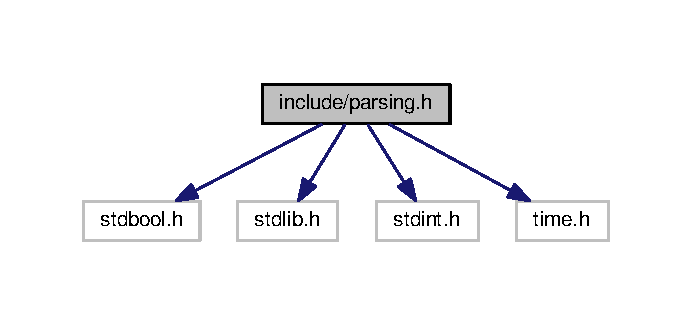
\includegraphics[width=332pt]{parsing_8h__incl}
\end{center}
\end{figure}
This graph shows which files directly or indirectly include this file\+:\nopagebreak
\begin{figure}[H]
\begin{center}
\leavevmode
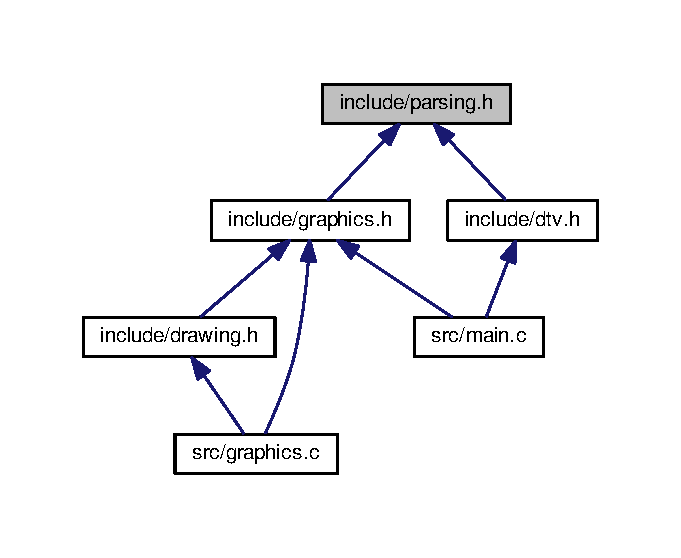
\includegraphics[width=266pt]{parsing_8h__dep__incl}
\end{center}
\end{figure}
\subsection*{Data Structures}
\begin{DoxyCompactItemize}
\item 
struct \hyperlink{structpat}{pat}
\begin{DoxyCompactList}\small\item\em Contains important info from the P\+AT table. \end{DoxyCompactList}\item 
struct \hyperlink{structpat_1_1pmt__basic}{pat\+::pmt\+\_\+basic}
\begin{DoxyCompactList}\small\item\em Contains enough info to identify a P\+MT table. \end{DoxyCompactList}\item 
struct \hyperlink{structpmt}{pmt}
\begin{DoxyCompactList}\small\item\em Contains important info from the P\+MT table. \end{DoxyCompactList}\item 
struct \hyperlink{structsdt}{sdt}
\begin{DoxyCompactList}\small\item\em Contains important info from the S\+DT table. \end{DoxyCompactList}\end{DoxyCompactItemize}
\subsection*{Functions}
\begin{DoxyCompactItemize}
\item 
struct \hyperlink{structpat}{pat} \hyperlink{group__parsing_ga15422ae30e0e1e43a15691ec066fb50f}{parse\+\_\+pat} (const uint8\+\_\+t $\ast$buffer)
\begin{DoxyCompactList}\small\item\em Parses the given buffer as a P\+AT table. \end{DoxyCompactList}\item 
struct \hyperlink{structpmt}{pmt} \hyperlink{group__parsing_ga1b750ab710b8dd637d53f464889bc179}{parse\+\_\+pmt} (const uint8\+\_\+t $\ast$buffer)
\begin{DoxyCompactList}\small\item\em Parses the given buffer as a P\+MT table. \end{DoxyCompactList}\item 
struct tm \hyperlink{group__parsing_gaf17c5270835b375f54f4752583f65287}{parse\+\_\+tot} (const uint8\+\_\+t $\ast$buffer)
\begin{DoxyCompactList}\small\item\em Parses the given buffer as a T\+OT table and converts its info to C representation of time. \end{DoxyCompactList}\item 
struct \hyperlink{structsdt}{sdt} \hyperlink{group__parsing_ga675aeacd9c1963445cce9f2e78b6b2a1}{parse\+\_\+sdt} (const uint8\+\_\+t $\ast$buffer, uint16\+\_\+t \hyperlink{structures_8h_abcdde739cb26f5c6c2c0b87e83d1f421}{ch\+\_\+num})
\begin{DoxyCompactList}\small\item\em Parses the given buffer as a S\+DT table and extracts information about the specified channel. \end{DoxyCompactList}\end{DoxyCompactItemize}


\subsection{Detailed Description}
Contains streamlined internal representations of tables. 


\hypertarget{rc_8h}{}\section{include/rc.h File Reference}
\label{rc_8h}\index{include/rc.\+h@{include/rc.\+h}}


Contains Remote Control A\+PI.  


{\ttfamily \#include \char`\"{}tdp\+\_\+api.\+h\char`\"{}}\\*
Include dependency graph for rc.\+h\+:\nopagebreak
\begin{figure}[H]
\begin{center}
\leavevmode
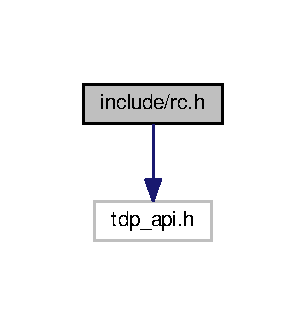
\includegraphics[width=147pt]{rc_8h__incl}
\end{center}
\end{figure}
This graph shows which files directly or indirectly include this file\+:\nopagebreak
\begin{figure}[H]
\begin{center}
\leavevmode
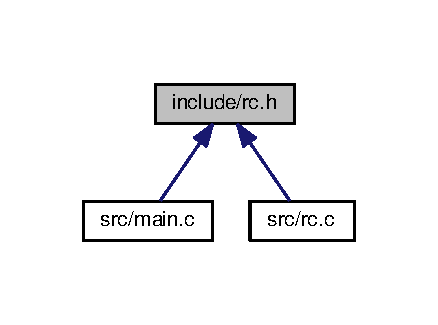
\includegraphics[width=210pt]{rc_8h__dep__incl}
\end{center}
\end{figure}
\subsection*{Macros}
\begin{DoxyCompactItemize}
\item 
\#define \hyperlink{rc_8h_ad79ba6770b2ab25b890f7819357a125d}{K\+E\+Y\+\_\+\+B\+A\+CK}~1\hypertarget{rc_8h_ad79ba6770b2ab25b890f7819357a125d}{}\label{rc_8h_ad79ba6770b2ab25b890f7819357a125d}

\begin{DoxyCompactList}\small\item\em Specifies the code of the back key. \end{DoxyCompactList}\item 
\#define \hyperlink{rc_8h_a5a7fd35018971faa28dacd3e33a8f737}{K\+E\+Y\+\_\+1}~2\hypertarget{rc_8h_a5a7fd35018971faa28dacd3e33a8f737}{}\label{rc_8h_a5a7fd35018971faa28dacd3e33a8f737}

\begin{DoxyCompactList}\small\item\em Specifies the code of the 1 key. \end{DoxyCompactList}\item 
\#define \hyperlink{rc_8h_a51ca76d1508339b071a974798b90474b}{K\+E\+Y\+\_\+0}~11\hypertarget{rc_8h_a51ca76d1508339b071a974798b90474b}{}\label{rc_8h_a51ca76d1508339b071a974798b90474b}

\begin{DoxyCompactList}\small\item\em Specifies the code of the 0 key. \end{DoxyCompactList}\item 
\#define \hyperlink{rc_8h_a222c823dcaa3e4638edf14e5d0b102d1}{K\+E\+Y\+\_\+\+M\+U\+TE}~60\hypertarget{rc_8h_a222c823dcaa3e4638edf14e5d0b102d1}{}\label{rc_8h_a222c823dcaa3e4638edf14e5d0b102d1}

\begin{DoxyCompactList}\small\item\em Specifies the code of the mute key. \end{DoxyCompactList}\item 
\#define \hyperlink{rc_8h_a6a5ca0598ce4e46d6bf0766b3da20aa7}{K\+E\+Y\+\_\+\+C\+H\+A\+N\+N\+E\+L\+\_\+\+D\+O\+WN}~61\hypertarget{rc_8h_a6a5ca0598ce4e46d6bf0766b3da20aa7}{}\label{rc_8h_a6a5ca0598ce4e46d6bf0766b3da20aa7}

\begin{DoxyCompactList}\small\item\em Specifies the code of the channel down key. \end{DoxyCompactList}\item 
\#define \hyperlink{rc_8h_ae3f801e1571016a4e9a344cb966de9a5}{K\+E\+Y\+\_\+\+C\+H\+A\+N\+N\+E\+L\+\_\+\+UP}~62\hypertarget{rc_8h_ae3f801e1571016a4e9a344cb966de9a5}{}\label{rc_8h_ae3f801e1571016a4e9a344cb966de9a5}

\begin{DoxyCompactList}\small\item\em Specifies the code of the channelup key. \end{DoxyCompactList}\item 
\#define \hyperlink{rc_8h_a476a0201859679ecc47815a321476c29}{K\+E\+Y\+\_\+\+V\+O\+L\+U\+M\+E\+\_\+\+UP}~63\hypertarget{rc_8h_a476a0201859679ecc47815a321476c29}{}\label{rc_8h_a476a0201859679ecc47815a321476c29}

\begin{DoxyCompactList}\small\item\em Specifies the code of the volume up key. \end{DoxyCompactList}\item 
\#define \hyperlink{rc_8h_a9ac8047db7d6b2c9e1514bba8dfbda28}{K\+E\+Y\+\_\+\+V\+O\+L\+U\+M\+E\+\_\+\+D\+O\+WN}~64\hypertarget{rc_8h_a9ac8047db7d6b2c9e1514bba8dfbda28}{}\label{rc_8h_a9ac8047db7d6b2c9e1514bba8dfbda28}

\begin{DoxyCompactList}\small\item\em Specifies the code of the volume down key. \end{DoxyCompactList}\item 
\#define \hyperlink{rc_8h_a0660be25c82280ce01d0bdaaf97e1e44}{K\+E\+Y\+\_\+\+I\+N\+FO}~358\hypertarget{rc_8h_a0660be25c82280ce01d0bdaaf97e1e44}{}\label{rc_8h_a0660be25c82280ce01d0bdaaf97e1e44}

\begin{DoxyCompactList}\small\item\em Specifies the code of the info key. \end{DoxyCompactList}\end{DoxyCompactItemize}
\subsection*{Typedefs}
\begin{DoxyCompactItemize}
\item 
typedef void($\ast$ \hyperlink{group__rc_gaa7ca8d3e24ef0c270366ce6fd9bcd258}{rc\+\_\+key\+\_\+callback}) (int key\+\_\+no)
\begin{DoxyCompactList}\small\item\em A callback that should take action on key press. \end{DoxyCompactList}\end{DoxyCompactItemize}
\subsection*{Functions}
\begin{DoxyCompactItemize}
\item 
void \hyperlink{group__rc_ga16d20af699334f6207d806701067ac96}{rc\+\_\+start\+\_\+loop} (const char $\ast$dev, \hyperlink{group__rc_gaa7ca8d3e24ef0c270366ce6fd9bcd258}{rc\+\_\+key\+\_\+callback} callback)
\begin{DoxyCompactList}\small\item\em A function that starts the loop that waits for input events from the remote control. \end{DoxyCompactList}\item 
void \hyperlink{group__rc_ga6d6de982bd06432345e8164a4c453fcc}{rc\+\_\+stop\+\_\+loop} ()
\begin{DoxyCompactList}\small\item\em Stops the event loop. \end{DoxyCompactList}\end{DoxyCompactItemize}


\subsection{Detailed Description}
Contains Remote Control A\+PI. 


\hypertarget{structures_8h}{}\section{include/structures.h File Reference}
\label{structures_8h}\index{include/structures.\+h@{include/structures.\+h}}


Contains nitty-\/gritty D\+VB details.  


{\ttfamily \#include $<$stdint.\+h$>$}\\*
Include dependency graph for structures.\+h\+:\nopagebreak
\begin{figure}[H]
\begin{center}
\leavevmode
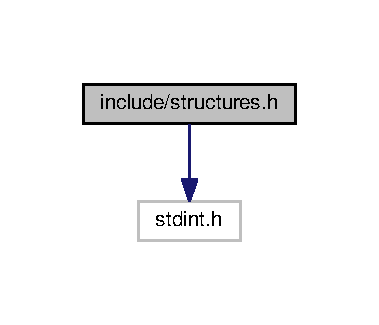
\includegraphics[width=182pt]{structures_8h__incl}
\end{center}
\end{figure}
\subsection*{Data Structures}
\begin{DoxyCompactItemize}
\item 
struct \hyperlink{structtable__header}{table\+\_\+header}
\begin{DoxyCompactList}\small\item\em Header that is part of all tables. \end{DoxyCompactList}\item 
struct \hyperlink{structpat__header}{pat\+\_\+header}
\begin{DoxyCompactList}\small\item\em Represents P\+AT header. \end{DoxyCompactList}\item 
struct \hyperlink{structpat__body}{pat\+\_\+body}
\begin{DoxyCompactList}\small\item\em Represents P\+AT body. \end{DoxyCompactList}\item 
struct \hyperlink{structpmt__header}{pmt\+\_\+header}
\begin{DoxyCompactList}\small\item\em Represents P\+MT header. \end{DoxyCompactList}\item 
struct \hyperlink{structpmt__body}{pmt\+\_\+body}
\begin{DoxyCompactList}\small\item\em Represents P\+MT body. \end{DoxyCompactList}\item 
struct \hyperlink{structteletext__descriptor__header}{teletext\+\_\+descriptor\+\_\+header}
\begin{DoxyCompactList}\small\item\em Represents the teletext descriptor header. \end{DoxyCompactList}\item 
struct \hyperlink{structsdt__header}{sdt\+\_\+header}
\begin{DoxyCompactList}\small\item\em Represents S\+DT header. \end{DoxyCompactList}\item 
struct \hyperlink{structsdt__body}{sdt\+\_\+body}
\begin{DoxyCompactList}\small\item\em Represents S\+DT body. \end{DoxyCompactList}\item 
struct \hyperlink{structsdt__descriptor1}{sdt\+\_\+descriptor1}
\begin{DoxyCompactList}\small\item\em Represents the first half of the service descriptor. \end{DoxyCompactList}\item 
struct \hyperlink{structsdt__descriptor2}{sdt\+\_\+descriptor2}
\begin{DoxyCompactList}\small\item\em Represents the second half of the service descriptor. \end{DoxyCompactList}\item 
struct \hyperlink{structtot__header}{tot\+\_\+header}
\begin{DoxyCompactList}\small\item\em Represents T\+OT header. \end{DoxyCompactList}\item 
struct \hyperlink{structtot__descriptor__header}{tot\+\_\+descriptor\+\_\+header}
\begin{DoxyCompactList}\small\item\em Represents T\+OT descriptor header. \end{DoxyCompactList}\item 
struct \hyperlink{structtot__descriptor__body}{tot\+\_\+descriptor\+\_\+body}
\begin{DoxyCompactList}\small\item\em Represents T\+OT descriptor body. \end{DoxyCompactList}\end{DoxyCompactItemize}
\subsection*{Functions}
\begin{DoxyCompactItemize}
\item 
struct \hyperlink{structtable__header}{table\+\_\+header} {\bfseries \+\_\+\+\_\+attribute\+\_\+\+\_\+} ((packed))
\item 
struct \hyperlink{structpat__header}{pat\+\_\+header} \hyperlink{group__structure_ga251eb9b1a59ade4a6230b32bdb6d83b1}{get\+\_\+pat\+\_\+header} (const uint8\+\_\+t $\ast$buffer)
\begin{DoxyCompactList}\small\item\em Retrieves \hyperlink{structpat__header}{pat\+\_\+header} from the stream. \end{DoxyCompactList}\item 
struct \hyperlink{structpat__body}{pat\+\_\+body} \hyperlink{group__structure_gac40b4dc77494cdc5b83144784224ad4a}{get\+\_\+pat\+\_\+body} (const uint8\+\_\+t $\ast$buffer)
\begin{DoxyCompactList}\small\item\em Retrieves \hyperlink{structpat__body}{pat\+\_\+body} from the stream. \end{DoxyCompactList}\item 
struct \hyperlink{structpmt__header}{pmt\+\_\+header} \hyperlink{group__structure_gaf0918f359410beb3897aee11d8bf1334}{get\+\_\+pmt\+\_\+header} (const uint8\+\_\+t $\ast$buffer)
\begin{DoxyCompactList}\small\item\em Retrieves \hyperlink{structpmt__header}{pmt\+\_\+header} from the stream. \end{DoxyCompactList}\item 
struct \hyperlink{structpmt__body}{pmt\+\_\+body} \hyperlink{group__structure_gae658cd1a590981159afcdd22a715837f}{get\+\_\+pmt\+\_\+body} (const uint8\+\_\+t $\ast$buffer)
\begin{DoxyCompactList}\small\item\em Retrieves \hyperlink{structpmt__body}{pmt\+\_\+body} from the stream. \end{DoxyCompactList}\item 
struct \hyperlink{structteletext__descriptor__header}{teletext\+\_\+descriptor\+\_\+header} \hyperlink{group__structure_gafbe380702060a8096a8c693c32294bf9}{get\+\_\+teletext\+\_\+descriptor\+\_\+header} (const uint8\+\_\+t $\ast$buffer)
\begin{DoxyCompactList}\small\item\em Retrieves \hyperlink{structteletext__descriptor__header}{teletext\+\_\+descriptor\+\_\+header} from the stream. \end{DoxyCompactList}\item 
struct \hyperlink{structsdt__header}{sdt\+\_\+header} \hyperlink{group__structure_ga8dccc2fbbab4df8588ea3f4154cd661a}{get\+\_\+sdt\+\_\+header} (const uint8\+\_\+t $\ast$buffer)
\begin{DoxyCompactList}\small\item\em Retrieves \hyperlink{structsdt__header}{sdt\+\_\+header} from the stream. \end{DoxyCompactList}\item 
struct \hyperlink{structsdt__body}{sdt\+\_\+body} \hyperlink{group__structure_gae8b16533467e7fb2a1c53b103a52542d}{get\+\_\+sdt\+\_\+body} (const uint8\+\_\+t $\ast$buffer)
\begin{DoxyCompactList}\small\item\em Retrieves \hyperlink{structsdt__body}{sdt\+\_\+body} from the stream. \end{DoxyCompactList}\item 
struct \hyperlink{structsdt__descriptor1}{sdt\+\_\+descriptor1} \hyperlink{group__structure_ga5df466f6e5e2fbd311ce4478f2693501}{get\+\_\+sdt\+\_\+descriptor1} (const uint8\+\_\+t $\ast$buffer)
\begin{DoxyCompactList}\small\item\em Retrieves \hyperlink{structsdt__descriptor1}{sdt\+\_\+descriptor1} from the stream. \end{DoxyCompactList}\item 
struct \hyperlink{structsdt__descriptor2}{sdt\+\_\+descriptor2} \hyperlink{group__structure_gaf3c5355cc1713bbc5648511e06058627}{get\+\_\+sdt\+\_\+descriptor2} (const uint8\+\_\+t $\ast$buffer)
\begin{DoxyCompactList}\small\item\em Retrieves \hyperlink{structsdt__descriptor2}{sdt\+\_\+descriptor2} from the stream. \end{DoxyCompactList}\item 
struct \hyperlink{structtot__header}{tot\+\_\+header} \hyperlink{group__structure_ga1a559bff189dc6665fbe0a18373868c0}{get\+\_\+tot\+\_\+header} (const uint8\+\_\+t $\ast$buffer)
\begin{DoxyCompactList}\small\item\em Retrieves \hyperlink{structtot__header}{tot\+\_\+header} from the stream. \end{DoxyCompactList}\item 
struct \hyperlink{structtot__descriptor__header}{tot\+\_\+descriptor\+\_\+header} \hyperlink{group__structure_gac4d9385a215e5da728266f73841f0db3}{get\+\_\+tot\+\_\+descriptor\+\_\+header} (const uint8\+\_\+t $\ast$buffer)
\begin{DoxyCompactList}\small\item\em Retrieves \hyperlink{structtot__descriptor__header}{tot\+\_\+descriptor\+\_\+header} from the stream. \end{DoxyCompactList}\item 
struct \hyperlink{structtot__descriptor__body}{tot\+\_\+descriptor\+\_\+body} \hyperlink{group__structure_ga4b0d2feed4e5af5e0a842dded06ef469}{get\+\_\+tot\+\_\+descriptor\+\_\+body} (const uint8\+\_\+t $\ast$buffer)
\begin{DoxyCompactList}\small\item\em Retrieves \hyperlink{structtot__descriptor__body}{tot\+\_\+descriptor\+\_\+body} from the stream. \end{DoxyCompactList}\end{DoxyCompactItemize}
\subsection*{Variables}
\begin{DoxyCompactItemize}
\item 
uint8\+\_\+t \hyperlink{structures_8h_a6f1dddf458f4e57fe3444309a958c73a}{tid}\hypertarget{structures_8h_a6f1dddf458f4e57fe3444309a958c73a}{}\label{structures_8h_a6f1dddf458f4e57fe3444309a958c73a}

\begin{DoxyCompactList}\small\item\em Table id. \end{DoxyCompactList}\item 
\begin{tabbing}
xx\=xx\=xx\=xx\=xx\=xx\=xx\=xx\=xx\=\kill
union \{\\
\>struct \{\\
\>\>uint16\_t \hyperlink{structures_8h_a5723e60ffd628510c699eddbce90be23}{len}: 12\\
\>\>\>{\em Length of the rest of the table. }\\
\>\>uint16\_t {\bfseries res}: 2\\
\>\>uint16\_t {\bfseries zero}: 1\\
\>\>uint16\_t {\bfseries ssi}: 1\\
\>\} {\bfseries b1s}\\
\>uint16\_t {\bfseries bitfield1}\\
\} {\bfseries b1u}\hypertarget{structures_8h_a7c2627052dc365d6992cee48817b5592}{}\label{structures_8h_a7c2627052dc365d6992cee48817b5592}
\\

\end{tabbing}\item 
struct \hyperlink{structtable__header}{table\+\_\+header} {\bfseries hdr}\hypertarget{structures_8h_acfb7f6dc69d6a8acc2709e1a05c5b43f}{}\label{structures_8h_acfb7f6dc69d6a8acc2709e1a05c5b43f}

\item 
uint16\+\_\+t {\bfseries tsi}\hypertarget{structures_8h_abed22e95934a64c8a46234a29cd64ff7}{}\label{structures_8h_abed22e95934a64c8a46234a29cd64ff7}

\item 
uint8\+\_\+t {\bfseries sec}\hypertarget{structures_8h_ad1696900026b287a87c563b733a21bc3}{}\label{structures_8h_ad1696900026b287a87c563b733a21bc3}

\item 
uint8\+\_\+t {\bfseries lsn}\hypertarget{structures_8h_acf8bf5a5f1df1204006643e403b5a977}{}\label{structures_8h_acf8bf5a5f1df1204006643e403b5a977}

\item 
uint16\+\_\+t \hyperlink{structures_8h_abcdde739cb26f5c6c2c0b87e83d1f421}{ch\+\_\+num}
\begin{DoxyCompactList}\small\item\em Channel number of the current P\+MT. \end{DoxyCompactList}\item 
\begin{tabbing}
xx\=xx\=xx\=xx\=xx\=xx\=xx\=xx\=xx\=\kill
struct \{\\
\>uint8\_t {\bfseries cni}: 1\\
\>uint8\_t {\bfseries version}: 5\\
\>uint8\_t {\bfseries res}: 2\\
\} {\bfseries b}\hypertarget{structures_8h_a9f4f8f956dfbaca1de306c85502305c9}{}\label{structures_8h_a9f4f8f956dfbaca1de306c85502305c9}
\\

\end{tabbing}\item 
\begin{tabbing}
xx\=xx\=xx\=xx\=xx\=xx\=xx\=xx\=xx\=\kill
union \{\\
\>struct \{\\
\>\>uint16\_t \hyperlink{structures_8h_a43608f79b946eb0b1ee920012497cd56}{pilen}: 12\\
\>\>\>{\em Length of the \hyperlink{structpmt__body}{pmt\_body} section. }\\
\>\>uint16\_t {\bfseries res3}: 4\\
\>\} {\bfseries b2s}\\
\>uint16\_t {\bfseries bitfield2}\\
\} {\bfseries b2u}\hypertarget{structures_8h_a5ae7e39b693ee6fc008952410d42796f}{}\label{structures_8h_a5ae7e39b693ee6fc008952410d42796f}
\\

\end{tabbing}\item 
uint8\+\_\+t \hyperlink{structures_8h_a1d127017fb298b889f4ba24752d08b8e}{type}
\begin{DoxyCompactList}\small\item\em Type of stream. \end{DoxyCompactList}\item 
struct \hyperlink{structteletext__descriptor__header}{teletext\+\_\+descriptor\+\_\+header} {\bfseries \+\_\+\+\_\+attribute\+\_\+\+\_\+}
\item 
uint16\+\_\+t {\bfseries oni}\hypertarget{structures_8h_acb6b38ae49635f2f5b5c89974037d65c}{}\label{structures_8h_acb6b38ae49635f2f5b5c89974037d65c}

\item 
uint16\+\_\+t \hyperlink{structures_8h_aa59e5e48a856ba2a010bb5447f79dbbb}{sid}\hypertarget{structures_8h_aa59e5e48a856ba2a010bb5447f79dbbb}{}\label{structures_8h_aa59e5e48a856ba2a010bb5447f79dbbb}

\begin{DoxyCompactList}\small\item\em Service id (same as channel number). \end{DoxyCompactList}\item 
uint8\+\_\+t {\bfseries tag}\hypertarget{structures_8h_a50ffde9be79dd080d9e8effe3ee52d66}{}\label{structures_8h_a50ffde9be79dd080d9e8effe3ee52d66}

\item 
uint8\+\_\+t \hyperlink{structures_8h_aa0f57098f04f59828e61140584f69fb1}{spnlen}\hypertarget{structures_8h_aa0f57098f04f59828e61140584f69fb1}{}\label{structures_8h_aa0f57098f04f59828e61140584f69fb1}

\begin{DoxyCompactList}\small\item\em Length of the service provider name. \end{DoxyCompactList}\item 
uint8\+\_\+t \hyperlink{structures_8h_a73f1800dbbe09690f1f45bcc2e560236}{snlen}\hypertarget{structures_8h_a73f1800dbbe09690f1f45bcc2e560236}{}\label{structures_8h_a73f1800dbbe09690f1f45bcc2e560236}

\begin{DoxyCompactList}\small\item\em Length of the service name. \end{DoxyCompactList}\item 
uint8\+\_\+t \hyperlink{structures_8h_a2f9f6d70359ec15fe3f50f1909636a90}{time} \mbox{[}5\mbox{]}\hypertarget{structures_8h_a2f9f6d70359ec15fe3f50f1909636a90}{}\label{structures_8h_a2f9f6d70359ec15fe3f50f1909636a90}

\begin{DoxyCompactList}\small\item\em Brain-\/dead encoded time information. \end{DoxyCompactList}\item 
uint16\+\_\+t \hyperlink{structures_8h_ae880b80206885df092c53d4aef122e44}{lto}\hypertarget{structures_8h_ae880b80206885df092c53d4aef122e44}{}\label{structures_8h_ae880b80206885df092c53d4aef122e44}

\begin{DoxyCompactList}\small\item\em Local time offset. \end{DoxyCompactList}\item 
uint8\+\_\+t {\bfseries toc} \mbox{[}5\mbox{]}\hypertarget{structures_8h_a93261cc350a49481bb3737b19e89fcea}{}\label{structures_8h_a93261cc350a49481bb3737b19e89fcea}

\item 
uint16\+\_\+t {\bfseries nto}\hypertarget{structures_8h_a075e40dfcaf09b8e3edf0b1d0e77461e}{}\label{structures_8h_a075e40dfcaf09b8e3edf0b1d0e77461e}

\end{DoxyCompactItemize}


\subsection{Detailed Description}
Contains nitty-\/gritty D\+VB details. 



\subsection{Variable Documentation}
\index{structures.\+h@{structures.\+h}!ch\+\_\+num@{ch\+\_\+num}}
\index{ch\+\_\+num@{ch\+\_\+num}!structures.\+h@{structures.\+h}}
\subsubsection[{\texorpdfstring{ch\+\_\+num}{ch_num}}]{\setlength{\rightskip}{0pt plus 5cm}uint16\+\_\+t ch\+\_\+num}\hypertarget{structures_8h_abcdde739cb26f5c6c2c0b87e83d1f421}{}\label{structures_8h_abcdde739cb26f5c6c2c0b87e83d1f421}


Channel number of the current P\+MT. 

Channel number. \index{structures.\+h@{structures.\+h}!len@{len}}
\index{len@{len}!structures.\+h@{structures.\+h}}
\subsubsection[{\texorpdfstring{len}{len}}]{\setlength{\rightskip}{0pt plus 5cm}uint8\+\_\+t len}\hypertarget{structures_8h_a5723e60ffd628510c699eddbce90be23}{}\label{structures_8h_a5723e60ffd628510c699eddbce90be23}


Length of the rest of the table. 

Length of the descriptor body.

Length of the descriptor. \index{structures.\+h@{structures.\+h}!pid@{pid}}
\index{pid@{pid}!structures.\+h@{structures.\+h}}
\subsubsection[{\texorpdfstring{pid}{pid}}]{\setlength{\rightskip}{0pt plus 5cm}uint16\+\_\+t pid}\hypertarget{structures_8h_a9089e9c40db82122a499b9620e2cb54e}{}\label{structures_8h_a9089e9c40db82122a499b9620e2cb54e}


P\+ID of the P\+MT table. 

P\+ID of the PS. \index{structures.\+h@{structures.\+h}!type@{type}}
\index{type@{type}!structures.\+h@{structures.\+h}}
\subsubsection[{\texorpdfstring{type}{type}}]{\setlength{\rightskip}{0pt plus 5cm}uint8\+\_\+t type}\hypertarget{structures_8h_a1d127017fb298b889f4ba24752d08b8e}{}\label{structures_8h_a1d127017fb298b889f4ba24752d08b8e}


Type of stream. 

Type of service (channel). 
\hypertarget{config_8c}{}\section{src/config.c File Reference}
\label{config_8c}\index{src/config.\+c@{src/config.\+c}}


Implementation for the configuration file interface.  


{\ttfamily \#include \char`\"{}config.\+h\char`\"{}}\\*
{\ttfamily \#include $<$inttypes.\+h$>$}\\*
{\ttfamily \#include $<$stdio.\+h$>$}\\*
{\ttfamily \#include $<$stdint.\+h$>$}\\*
{\ttfamily \#include \char`\"{}tdp\+\_\+api.\+h\char`\"{}}\\*
Include dependency graph for config.\+c\+:\nopagebreak
\begin{figure}[H]
\begin{center}
\leavevmode
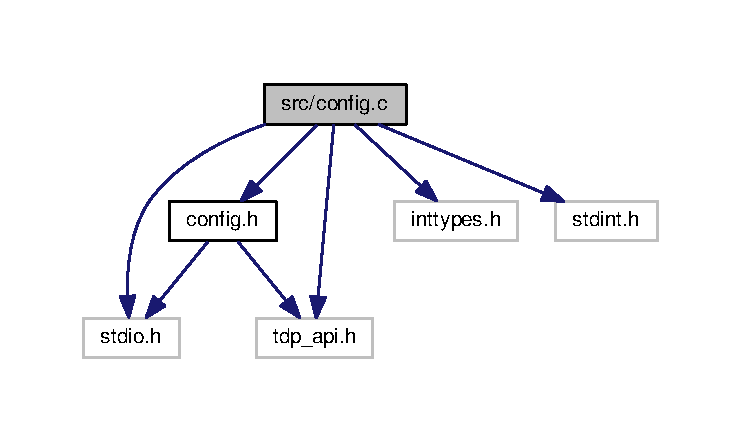
\includegraphics[width=350pt]{config_8c__incl}
\end{center}
\end{figure}
\subsection*{Macros}
\begin{DoxyCompactItemize}
\item 
\#define \hyperlink{config_8c_a6821bafc3c88dfb2e433a095df9940c6}{B\+U\+F\+\_\+\+S\+I\+ZE}~100
\item 
\#define \hyperlink{config_8c_a73e900891c40d086984338bdb587270b}{M\+A\+K\+E\+\_\+\+G\+E\+T\+T\+ER}(T\+Y\+PE,  N\+A\+ME,  N\+O\+T\+\_\+\+F\+O\+U\+ND,  C\+O\+N\+V\+E\+R\+S\+I\+ON)
\begin{DoxyCompactList}\small\item\em Creates a getter function for a field. The generated function is named get\+\_\+\+N\+A\+ME, and searches through the file, for the field N\+A\+ME, with type T\+Y\+PE, and input conversion C\+O\+N\+V\+E\+R\+S\+I\+ON. \end{DoxyCompactList}\end{DoxyCompactItemize}
\subsection*{Functions}
\begin{DoxyCompactItemize}
\item 
\hyperlink{config_8c_a749f05febee67a1cc32e3d2141561414}{M\+A\+K\+E\+\_\+\+G\+E\+T\+T\+ER} (uint32\+\_\+t, frequency, N\+O\+\_\+\+F\+R\+E\+Q\+U\+E\+N\+CY,\char`\"{}\%\char`\"{}S\+C\+Nu32)\hypertarget{config_8c_a749f05febee67a1cc32e3d2141561414}{}\label{config_8c_a749f05febee67a1cc32e3d2141561414}

\begin{DoxyCompactList}\small\item\em Attempts to load frequency from file. \end{DoxyCompactList}\item 
\hyperlink{config_8c_ac9993275589f8863d8b2cec36a151a8d}{M\+A\+K\+E\+\_\+\+G\+E\+T\+T\+ER} (uint32\+\_\+t, bandwidth, N\+O\+\_\+\+B\+A\+N\+D\+W\+I\+D\+TH,\char`\"{}\%\char`\"{}S\+C\+Nu32)\hypertarget{config_8c_ac9993275589f8863d8b2cec36a151a8d}{}\label{config_8c_ac9993275589f8863d8b2cec36a151a8d}

\begin{DoxyCompactList}\small\item\em Attempts to load bandwidth from file. \end{DoxyCompactList}\item 
\hyperlink{config_8c_a9aeda71de4e31859c1a7af2dc0ba654f}{M\+A\+K\+E\+\_\+\+G\+E\+T\+T\+ER} (uint16\+\_\+t, video\+\_\+pid, N\+O\+\_\+\+V\+I\+D\+E\+O\+\_\+\+P\+ID,\char`\"{}\%\char`\"{}S\+C\+Nu16)\hypertarget{config_8c_a9aeda71de4e31859c1a7af2dc0ba654f}{}\label{config_8c_a9aeda71de4e31859c1a7af2dc0ba654f}

\begin{DoxyCompactList}\small\item\em Attempts to load video P\+ID from file. \end{DoxyCompactList}\item 
\hyperlink{config_8c_a1dc6cc472e5f6554581ae29cfbfb597b}{M\+A\+K\+E\+\_\+\+G\+E\+T\+T\+ER} (uint16\+\_\+t, audio\+\_\+pid, N\+O\+\_\+\+A\+U\+D\+I\+O\+\_\+\+P\+ID,\char`\"{}\%\char`\"{}S\+C\+Nu16)\hypertarget{config_8c_a1dc6cc472e5f6554581ae29cfbfb597b}{}\label{config_8c_a1dc6cc472e5f6554581ae29cfbfb597b}

\begin{DoxyCompactList}\small\item\em Attempts to load audio P\+ID from file. \end{DoxyCompactList}\item 
\hyperlink{config_8c_a0d86b42ab3a09de149ae3f8b47af516a}{M\+A\+K\+E\+\_\+\+G\+E\+T\+T\+ER} (uint16\+\_\+t, \hyperlink{structures_8h_abcdde739cb26f5c6c2c0b87e83d1f421}{ch\+\_\+num}, N\+O\+\_\+\+C\+H\+\_\+\+N\+UM,\char`\"{}\%\char`\"{}S\+C\+Nu16)\hypertarget{config_8c_a0d86b42ab3a09de149ae3f8b47af516a}{}\label{config_8c_a0d86b42ab3a09de149ae3f8b47af516a}

\begin{DoxyCompactList}\small\item\em Attempts to load channel number from file. \end{DoxyCompactList}\item 
\hyperlink{config_8c_a988fcd0abc704e9d3af03d840a426393}{M\+A\+K\+E\+\_\+\+G\+E\+T\+T\+ER} (int, module, N\+O\+\_\+\+M\+O\+D\+U\+LE,\char`\"{}\%d\char`\"{})\hypertarget{config_8c_a988fcd0abc704e9d3af03d840a426393}{}\label{config_8c_a988fcd0abc704e9d3af03d840a426393}

\begin{DoxyCompactList}\small\item\em Attempts to load module type from file. \end{DoxyCompactList}\item 
\hyperlink{config_8c_a2bef078a01875edb5403d6cd1c4b0cab}{M\+A\+K\+E\+\_\+\+G\+E\+T\+T\+ER} (int, video\+\_\+type, N\+O\+\_\+\+V\+I\+D\+E\+O\+\_\+\+T\+Y\+PE,\char`\"{}\%d\char`\"{})\hypertarget{config_8c_a2bef078a01875edb5403d6cd1c4b0cab}{}\label{config_8c_a2bef078a01875edb5403d6cd1c4b0cab}

\begin{DoxyCompactList}\small\item\em Attempts to load video type from file. \end{DoxyCompactList}\item 
\hyperlink{config_8c_ad0b1b545727615f439cd1d8da5f0cdf7}{M\+A\+K\+E\+\_\+\+G\+E\+T\+T\+ER} (int, audio\+\_\+type, N\+O\+\_\+\+A\+U\+D\+I\+O\+\_\+\+T\+Y\+PE,\char`\"{}\%d\char`\"{})\hypertarget{config_8c_ad0b1b545727615f439cd1d8da5f0cdf7}{}\label{config_8c_ad0b1b545727615f439cd1d8da5f0cdf7}

\begin{DoxyCompactList}\small\item\em Attempts to load audio type from file. \end{DoxyCompactList}\item 
\hyperlink{config_8c_a670ef589443019e66fc5d4b9a967746d}{M\+A\+K\+E\+\_\+\+G\+E\+T\+T\+ER} (int, teletext, N\+O\+\_\+\+T\+E\+L\+E\+T\+E\+XT,\char`\"{}\%d\char`\"{})\hypertarget{config_8c_a670ef589443019e66fc5d4b9a967746d}{}\label{config_8c_a670ef589443019e66fc5d4b9a967746d}

\begin{DoxyCompactList}\small\item\em Attempts t oload teletext from file. \end{DoxyCompactList}\item 
struct \hyperlink{structconfig__init__ch__info}{config\+\_\+init\+\_\+ch\+\_\+info} \hyperlink{group__config_gad7d820530151b1bb2b6cf6e992f48331}{config\+\_\+get\+\_\+init\+\_\+ch\+\_\+info} (F\+I\+LE $\ast$f)
\begin{DoxyCompactList}\small\item\em Attempts to load all fields from the file. \end{DoxyCompactList}\end{DoxyCompactItemize}


\subsection{Detailed Description}
Implementation for the configuration file interface. 



\subsection{Macro Definition Documentation}
\index{config.\+c@{config.\+c}!B\+U\+F\+\_\+\+S\+I\+ZE@{B\+U\+F\+\_\+\+S\+I\+ZE}}
\index{B\+U\+F\+\_\+\+S\+I\+ZE@{B\+U\+F\+\_\+\+S\+I\+ZE}!config.\+c@{config.\+c}}
\subsubsection[{\texorpdfstring{B\+U\+F\+\_\+\+S\+I\+ZE}{BUF_SIZE}}]{\setlength{\rightskip}{0pt plus 5cm}\#define B\+U\+F\+\_\+\+S\+I\+ZE~100}\hypertarget{config_8c_a6821bafc3c88dfb2e433a095df9940c6}{}\label{config_8c_a6821bafc3c88dfb2e433a095df9940c6}

\begin{DoxyParams}{Parameters}
{\em Buffer} & size for reading the file. \\
\hline
\end{DoxyParams}
\index{config.\+c@{config.\+c}!M\+A\+K\+E\+\_\+\+G\+E\+T\+T\+ER@{M\+A\+K\+E\+\_\+\+G\+E\+T\+T\+ER}}
\index{M\+A\+K\+E\+\_\+\+G\+E\+T\+T\+ER@{M\+A\+K\+E\+\_\+\+G\+E\+T\+T\+ER}!config.\+c@{config.\+c}}
\subsubsection[{\texorpdfstring{M\+A\+K\+E\+\_\+\+G\+E\+T\+T\+ER}{MAKE_GETTER}}]{\setlength{\rightskip}{0pt plus 5cm}\#define M\+A\+K\+E\+\_\+\+G\+E\+T\+T\+ER(
\begin{DoxyParamCaption}
\item[{}]{T\+Y\+PE, }
\item[{}]{N\+A\+ME, }
\item[{}]{N\+O\+T\+\_\+\+F\+O\+U\+ND, }
\item[{}]{C\+O\+N\+V\+E\+R\+S\+I\+ON}
\end{DoxyParamCaption}
)}\hypertarget{config_8c_a73e900891c40d086984338bdb587270b}{}\label{config_8c_a73e900891c40d086984338bdb587270b}
{\bfseries Value\+:}
\begin{DoxyCode}
\textcolor{keyword}{static} TYPE get\_##NAME(FILE *f) \(\backslash\)
\{ \(\backslash\)
    rewind(f); \(\backslash\)
 \(\backslash\)
    while (!feof(f)) \(\backslash\)
    \{ \(\backslash\)
        char buf[\hyperlink{config_8c_a6821bafc3c88dfb2e433a095df9940c6}{BUF\_SIZE}]; \(\backslash\)
        fgets(buf, \hyperlink{config_8c_a6821bafc3c88dfb2e433a095df9940c6}{BUF\_SIZE}, f); \(\backslash\)
 \(\backslash\)
        TYPE ret; \(\backslash\)
        if (sscanf(buf, #NAME\textcolor{stringliteral}{" = "}CONVERSION, &ret) == 1) \(\backslash\)
            return ret; \(\backslash\)
    \} \(\backslash\)
 \(\backslash\)
    return NOT\_FOUND; \(\backslash\)
\}
\end{DoxyCode}


Creates a getter function for a field. The generated function is named get\+\_\+\+N\+A\+ME, and searches through the file, for the field N\+A\+ME, with type T\+Y\+PE, and input conversion C\+O\+N\+V\+E\+R\+S\+I\+ON. 


\begin{DoxyParams}{Parameters}
{\em T\+Y\+PE} & type of the field, and also return type of the function. \\
\hline
{\em N\+A\+ME} & name of the field, which is also part of the function name. \\
\hline
{\em N\+O\+T\+\_\+\+F\+O\+U\+ND} & value of type T\+Y\+PE, to be returned if field was not found. \\
\hline
{\em C\+O\+N\+V\+E\+R\+S\+I\+ON} & A compile-\/time string that specifies the input conversion à la scanf. \\
\hline
\end{DoxyParams}

\hypertarget{graphics_8c}{}\section{src/graphics.c File Reference}
\label{graphics_8c}\index{src/graphics.\+c@{src/graphics.\+c}}


Contains implementation for graphics interface.  


{\ttfamily \#include $<$stdint.\+h$>$}\\*
{\ttfamily \#include $<$stdio.\+h$>$}\\*
{\ttfamily \#include $<$time.\+h$>$}\\*
{\ttfamily \#include $<$pthread.\+h$>$}\\*
{\ttfamily \#include $<$signal.\+h$>$}\\*
{\ttfamily \#include $<$unistd.\+h$>$}\\*
{\ttfamily \#include $<$directfb.\+h$>$}\\*
{\ttfamily \#include \char`\"{}common.\+h\char`\"{}}\\*
{\ttfamily \#include \char`\"{}drawing.\+h\char`\"{}}\\*
{\ttfamily \#include \char`\"{}graphics.\+h\char`\"{}}\\*
Include dependency graph for graphics.\+c\+:\nopagebreak
\begin{figure}[H]
\begin{center}
\leavevmode
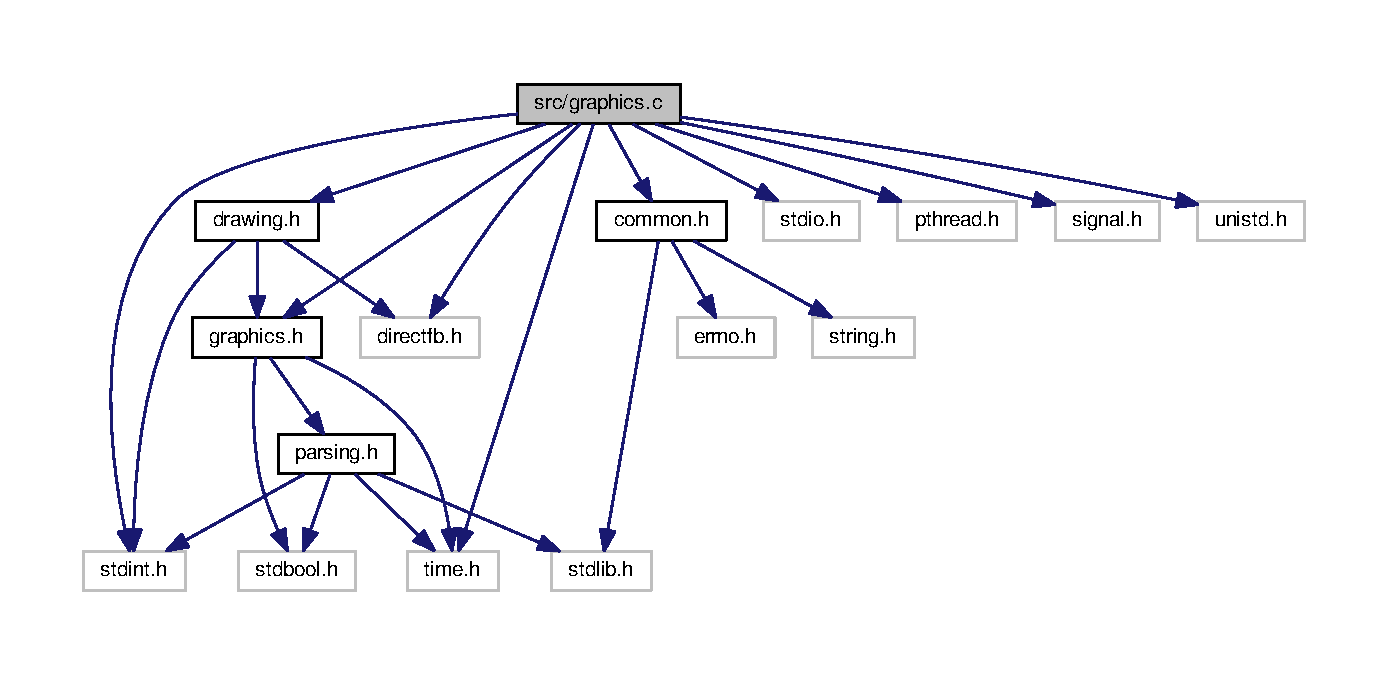
\includegraphics[width=350pt]{graphics_8c__incl}
\end{center}
\end{figure}
\subsection*{Data Structures}
\begin{DoxyCompactItemize}
\item 
struct \hyperlink{structgraphics__flags}{graphics\+\_\+flags}
\begin{DoxyCompactList}\small\item\em A struct that keeps the state of what should be displayed. \end{DoxyCompactList}\item 
struct \hyperlink{structargs}{args}
\begin{DoxyCompactList}\small\item\em A shim structure to pass main arguments to Direct\+FB. \end{DoxyCompactList}\end{DoxyCompactItemize}
\subsection*{Macros}
\begin{DoxyCompactItemize}
\item 
\#define {\bfseries \+\_\+\+P\+O\+S\+I\+X\+\_\+\+C\+\_\+\+S\+O\+U\+R\+CE}~200809L\hypertarget{graphics_8c_a3024ccd4a9af5109d24e6c57565d74a1}{}\label{graphics_8c_a3024ccd4a9af5109d24e6c57565d74a1}

\item 
\#define {\bfseries L\+O\+G\+\_\+\+G\+R\+A\+P\+H\+I\+CS}(fmt, ...)~\hyperlink{common_8h_ac464f11a32500a31842789297a3c31f4}{L\+OG}(\char`\"{}Graphics\char`\"{}, fmt, \#\#\+\_\+\+\_\+\+V\+A\+\_\+\+A\+R\+G\+S\+\_\+\+\_\+)\hypertarget{graphics_8c_ab3c493d3864c2625f36f4fa6eee278ba}{}\label{graphics_8c_ab3c493d3864c2625f36f4fa6eee278ba}

\item 
\#define {\bfseries D\+R\+A\+W\+C\+H\+E\+CK}(err)
\end{DoxyCompactItemize}
\subsection*{Enumerations}
\begin{DoxyCompactItemize}
\item 
enum \hyperlink{graphics_8c_a8f99466c4a0862f1c85496dfd103a237}{g\+\_\+error} \{ \hyperlink{graphics_8c_a8f99466c4a0862f1c85496dfd103a237a661f2f26115943a3c0afec6d2bb48d8f}{G\+\_\+\+E\+R\+R\+OR} = -\/1, 
\hyperlink{graphics_8c_a8f99466c4a0862f1c85496dfd103a237a5ba6282852db042c2f7dbb9b66cf9f70}{G\+\_\+\+N\+O\+\_\+\+E\+R\+R\+OR}
 \}\begin{DoxyCompactList}\small\item\em Error codes to be used for internal graphics functions. \end{DoxyCompactList}
\end{DoxyCompactItemize}
\subsection*{Functions}
\begin{DoxyCompactItemize}
\item 
void \hyperlink{group__graphics_ga741d634a2444a13cc83411c4bb98d948}{graphics\+\_\+show\+\_\+channel\+\_\+info} (struct \hyperlink{structgraphics__channel__info}{graphics\+\_\+channel\+\_\+info} info)
\begin{DoxyCompactList}\small\item\em Displays some basic information about a channel on the screen. \end{DoxyCompactList}\item 
void \hyperlink{group__graphics_ga9cfad8e0d3cdb8597e3f3a2bdfd3bfda}{graphics\+\_\+show\+\_\+time} (struct tm tm)
\begin{DoxyCompactList}\small\item\em Displays current time. \end{DoxyCompactList}\item 
void \hyperlink{group__graphics_gaf1c74824677854f7abe3e6590343580f}{graphics\+\_\+show\+\_\+volume} (uint8\+\_\+t vol)
\begin{DoxyCompactList}\small\item\em Displays volume information on the screen. \end{DoxyCompactList}\item 
void \hyperlink{group__graphics_ga07d069f854ed989682f48d8eb2b96392}{graphics\+\_\+show\+\_\+init} ()
\begin{DoxyCompactList}\small\item\em Displays initializing message. \end{DoxyCompactList}\item 
void \hyperlink{group__graphics_gaa14c15905aaa8584ac0d41629e63179e}{graphics\+\_\+hide\+\_\+init} ()
\begin{DoxyCompactList}\small\item\em Removes initializing message. \end{DoxyCompactList}\item 
void \hyperlink{group__graphics_ga88347b80264b415007253f935d32023c}{graphics\+\_\+show\+\_\+mute} ()
\begin{DoxyCompactList}\small\item\em Displays mute symbol. \end{DoxyCompactList}\item 
void \hyperlink{group__graphics_ga56554c1a2cf638c4a3804f36656a75f9}{graphics\+\_\+hide\+\_\+mute} ()
\begin{DoxyCompactList}\small\item\em Removes mute symbol. \end{DoxyCompactList}\item 
void \hyperlink{group__graphics_ga6832a9b03441e5a9d47d3c8e3e01a591}{graphics\+\_\+show\+\_\+channel\+\_\+number} (uint16\+\_\+t \hyperlink{structures_8h_abcdde739cb26f5c6c2c0b87e83d1f421}{ch\+\_\+num})
\begin{DoxyCompactList}\small\item\em Displays selected channel number. \end{DoxyCompactList}\item 
void \hyperlink{group__graphics_gac220b5d62d022399bb1e3a9cf6b1dce2}{graphics\+\_\+blackscreen} ()
\begin{DoxyCompactList}\small\item\em Puts a black screen on the screen. \end{DoxyCompactList}\item 
void \hyperlink{group__graphics_ga46d440f27511750ed679ec47c7491579}{graphics\+\_\+clear} ()
\begin{DoxyCompactList}\small\item\em Clears all graphics elements from screen. \end{DoxyCompactList}\item 
enum \hyperlink{graphics_8c_a8f99466c4a0862f1c85496dfd103a237}{g\+\_\+error} \hyperlink{graphics_8c_a5945a267b0c42c153e55a7f5d9d6be7a}{graphics\+\_\+render} (int $\ast$argc, char $\ast$$\ast$$\ast$argv)\hypertarget{graphics_8c_a5945a267b0c42c153e55a7f5d9d6be7a}{}\label{graphics_8c_a5945a267b0c42c153e55a7f5d9d6be7a}

\begin{DoxyCompactList}\small\item\em Function that continuously refreshes graphics display according to the current state of \hyperlink{structgraphics__flags}{graphics\+\_\+flags}. \end{DoxyCompactList}\item 
void \hyperlink{group__graphics_ga96cea86bf40f2181cadf6686b82f28a3}{graphics\+\_\+start\+\_\+render} (int $\ast$argc, char $\ast$$\ast$$\ast$argv)
\begin{DoxyCompactList}\small\item\em Starts rendering graphic elements on screen. \end{DoxyCompactList}\item 
void \hyperlink{group__graphics_ga0807641f1877b4586e9537144b80f6b6}{graphics\+\_\+stop} ()
\begin{DoxyCompactList}\small\item\em Stops graphics rendering loop. \end{DoxyCompactList}\end{DoxyCompactItemize}


\subsection{Detailed Description}
Contains implementation for graphics interface. 



\subsection{Macro Definition Documentation}
\index{graphics.\+c@{graphics.\+c}!D\+R\+A\+W\+C\+H\+E\+CK@{D\+R\+A\+W\+C\+H\+E\+CK}}
\index{D\+R\+A\+W\+C\+H\+E\+CK@{D\+R\+A\+W\+C\+H\+E\+CK}!graphics.\+c@{graphics.\+c}}
\subsubsection[{\texorpdfstring{D\+R\+A\+W\+C\+H\+E\+CK}{DRAWCHECK}}]{\setlength{\rightskip}{0pt plus 5cm}\#define D\+R\+A\+W\+C\+H\+E\+CK(
\begin{DoxyParamCaption}
\item[{}]{err}
\end{DoxyParamCaption}
)}\hypertarget{graphics_8c_a76ab2efd44713dd3a2df776d8cd153c7}{}\label{graphics_8c_a76ab2efd44713dd3a2df776d8cd153c7}
{\bfseries Value\+:}
\begin{DoxyCode}
\{ \(\backslash\)
    if (err != EXIT\_SUCCESS) \(\backslash\)
    \{ \(\backslash\)
        fprintf(stderr, \textcolor{stringliteral}{"%s:%d:%s\(\backslash\)n"}, \_\_FILE\_\_, \_\_LINE\_\_, \_\_func\_\_); \(\backslash\)
        release(); \(\backslash\)
        return \hyperlink{graphics_8c_a8f99466c4a0862f1c85496dfd103a237a661f2f26115943a3c0afec6d2bb48d8f}{G\_ERROR}; \(\backslash\)
     \} \(\backslash\)
\}
\end{DoxyCode}


\subsection{Enumeration Type Documentation}
\index{graphics.\+c@{graphics.\+c}!g\+\_\+error@{g\+\_\+error}}
\index{g\+\_\+error@{g\+\_\+error}!graphics.\+c@{graphics.\+c}}
\subsubsection[{\texorpdfstring{g\+\_\+error}{g_error}}]{\setlength{\rightskip}{0pt plus 5cm}enum {\bf g\+\_\+error}}\hypertarget{graphics_8c_a8f99466c4a0862f1c85496dfd103a237}{}\label{graphics_8c_a8f99466c4a0862f1c85496dfd103a237}


Error codes to be used for internal graphics functions. 

\begin{Desc}
\item[Enumerator]\par
\begin{description}
\index{G\+\_\+\+E\+R\+R\+OR@{G\+\_\+\+E\+R\+R\+OR}!graphics.\+c@{graphics.\+c}}\index{graphics.\+c@{graphics.\+c}!G\+\_\+\+E\+R\+R\+OR@{G\+\_\+\+E\+R\+R\+OR}}\item[{\em 
G\+\_\+\+E\+R\+R\+OR\hypertarget{graphics_8c_a8f99466c4a0862f1c85496dfd103a237a661f2f26115943a3c0afec6d2bb48d8f}{}\label{graphics_8c_a8f99466c4a0862f1c85496dfd103a237a661f2f26115943a3c0afec6d2bb48d8f}
}]Specifies that a graphics error has occurred. \index{G\+\_\+\+N\+O\+\_\+\+E\+R\+R\+OR@{G\+\_\+\+N\+O\+\_\+\+E\+R\+R\+OR}!graphics.\+c@{graphics.\+c}}\index{graphics.\+c@{graphics.\+c}!G\+\_\+\+N\+O\+\_\+\+E\+R\+R\+OR@{G\+\_\+\+N\+O\+\_\+\+E\+R\+R\+OR}}\item[{\em 
G\+\_\+\+N\+O\+\_\+\+E\+R\+R\+OR\hypertarget{graphics_8c_a8f99466c4a0862f1c85496dfd103a237a5ba6282852db042c2f7dbb9b66cf9f70}{}\label{graphics_8c_a8f99466c4a0862f1c85496dfd103a237a5ba6282852db042c2f7dbb9b66cf9f70}
}]Specifies that a graphics\+\_\+error has {\itshape not} occurred. \end{description}
\end{Desc}

\hypertarget{main_8c}{}\section{src/main.c File Reference}
\label{main_8c}\index{src/main.\+c@{src/main.\+c}}


Contains the implementation that glues other modules together.  


{\ttfamily \#include $<$stdbool.\+h$>$}\\*
{\ttfamily \#include $<$stdlib.\+h$>$}\\*
{\ttfamily \#include $<$stdio.\+h$>$}\\*
{\ttfamily \#include $<$time.\+h$>$}\\*
{\ttfamily \#include $<$pthread.\+h$>$}\\*
{\ttfamily \#include $<$signal.\+h$>$}\\*
{\ttfamily \#include $<$unistd.\+h$>$}\\*
{\ttfamily \#include \char`\"{}common.\+h\char`\"{}}\\*
{\ttfamily \#include \char`\"{}graphics.\+h\char`\"{}}\\*
{\ttfamily \#include \char`\"{}config.\+h\char`\"{}}\\*
{\ttfamily \#include \char`\"{}dtv.\+h\char`\"{}}\\*
{\ttfamily \#include \char`\"{}rc.\+h\char`\"{}}\\*
Include dependency graph for main.\+c\+:\nopagebreak
\begin{figure}[H]
\begin{center}
\leavevmode
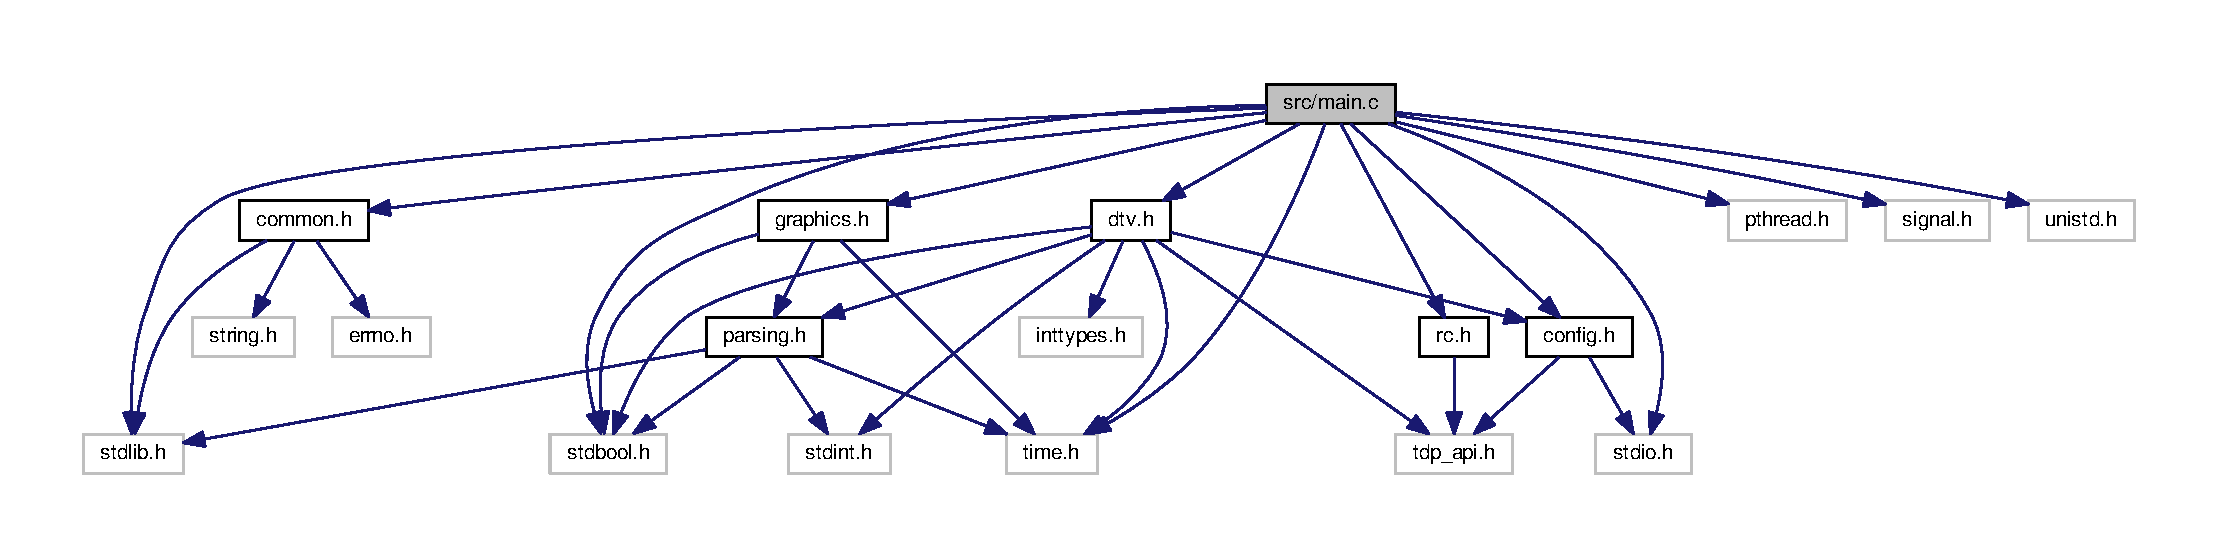
\includegraphics[width=350pt]{main_8c__incl}
\end{center}
\end{figure}
\subsection*{Macros}
\begin{DoxyCompactItemize}
\item 
\#define {\bfseries \+\_\+\+P\+O\+S\+I\+X\+\_\+\+C\+\_\+\+S\+O\+U\+R\+CE}~200809L\hypertarget{main_8c_a3024ccd4a9af5109d24e6c57565d74a1}{}\label{main_8c_a3024ccd4a9af5109d24e6c57565d74a1}

\item 
\#define {\bfseries L\+O\+G\+\_\+\+M\+A\+IN}(fmt, ...)~\hyperlink{common_8h_ac464f11a32500a31842789297a3c31f4}{L\+OG}(\char`\"{}Main\char`\"{}, fmt, \#\#\+\_\+\+\_\+\+V\+A\+\_\+\+A\+R\+G\+S\+\_\+\+\_\+)\hypertarget{main_8c_a03d48c884c8c9db8cb3413f3411c0a1e}{}\label{main_8c_a03d48c884c8c9db8cb3413f3411c0a1e}

\end{DoxyCompactItemize}
\subsection*{Functions}
\begin{DoxyCompactItemize}
\item 
void \hyperlink{main_8c_a2ac88a8040c89c43521f48e500eea700}{handle\+\_\+signal} (int signum)\hypertarget{main_8c_a2ac88a8040c89c43521f48e500eea700}{}\label{main_8c_a2ac88a8040c89c43521f48e500eea700}

\begin{DoxyCompactList}\small\item\em Function that handles S\+I\+G\+I\+NT and S\+I\+G\+T\+E\+RT, by ensuring graceful exit. \end{DoxyCompactList}\item 
void \hyperlink{main_8c_a73d711c2ea70f5243f68a2ecb7aa3698}{calculate\+\_\+time} ()\hypertarget{main_8c_a73d711c2ea70f5243f68a2ecb7aa3698}{}\label{main_8c_a73d711c2ea70f5243f68a2ecb7aa3698}

\begin{DoxyCompactList}\small\item\em Function that calculates the amount of time that has passed since T\+OT table was received, and adjusts the time to be displayed accordingly. \end{DoxyCompactList}\item 
void \hyperlink{main_8c_a4fdc17e5cad8065f01f410bf398756c5}{confirm\+\_\+channel} (union sigval s)\hypertarget{main_8c_a4fdc17e5cad8065f01f410bf398756c5}{}\label{main_8c_a4fdc17e5cad8065f01f410bf398756c5}

\begin{DoxyCompactList}\small\item\em Function that switches channels once the change has been confirmed. \end{DoxyCompactList}\item 
void \hyperlink{main_8c_af669e03dbaedb31097f0f42e857e9ff4}{react\+\_\+to\+\_\+keypress} (int key\+\_\+code)\hypertarget{main_8c_af669e03dbaedb31097f0f42e857e9ff4}{}\label{main_8c_af669e03dbaedb31097f0f42e857e9ff4}

\begin{DoxyCompactList}\small\item\em Function that reacts to a keypress from the remote control. \end{DoxyCompactList}\item 
int {\bfseries main} (int argc, char $\ast$$\ast$argv)\hypertarget{main_8c_a3c04138a5bfe5d72780bb7e82a18e627}{}\label{main_8c_a3c04138a5bfe5d72780bb7e82a18e627}

\end{DoxyCompactItemize}


\subsection{Detailed Description}
Contains the implementation that glues other modules together. 


\hypertarget{rc_8c}{}\section{src/rc.c File Reference}
\label{rc_8c}\index{src/rc.\+c@{src/rc.\+c}}


Contains the implementation of the remote control interface.  


{\ttfamily \#include \char`\"{}rc.\+h\char`\"{}}\\*
{\ttfamily \#include $<$errno.\+h$>$}\\*
{\ttfamily \#include $<$stdbool.\+h$>$}\\*
{\ttfamily \#include $<$stdlib.\+h$>$}\\*
{\ttfamily \#include $<$stdio.\+h$>$}\\*
{\ttfamily \#include $<$string.\+h$>$}\\*
{\ttfamily \#include $<$time.\+h$>$}\\*
{\ttfamily \#include $<$fcntl.\+h$>$}\\*
{\ttfamily \#include $<$pthread.\+h$>$}\\*
{\ttfamily \#include $<$unistd.\+h$>$}\\*
{\ttfamily \#include $<$linux/input.\+h$>$}\\*
{\ttfamily \#include \char`\"{}common.\+h\char`\"{}}\\*
Include dependency graph for rc.\+c\+:\nopagebreak
\begin{figure}[H]
\begin{center}
\leavevmode
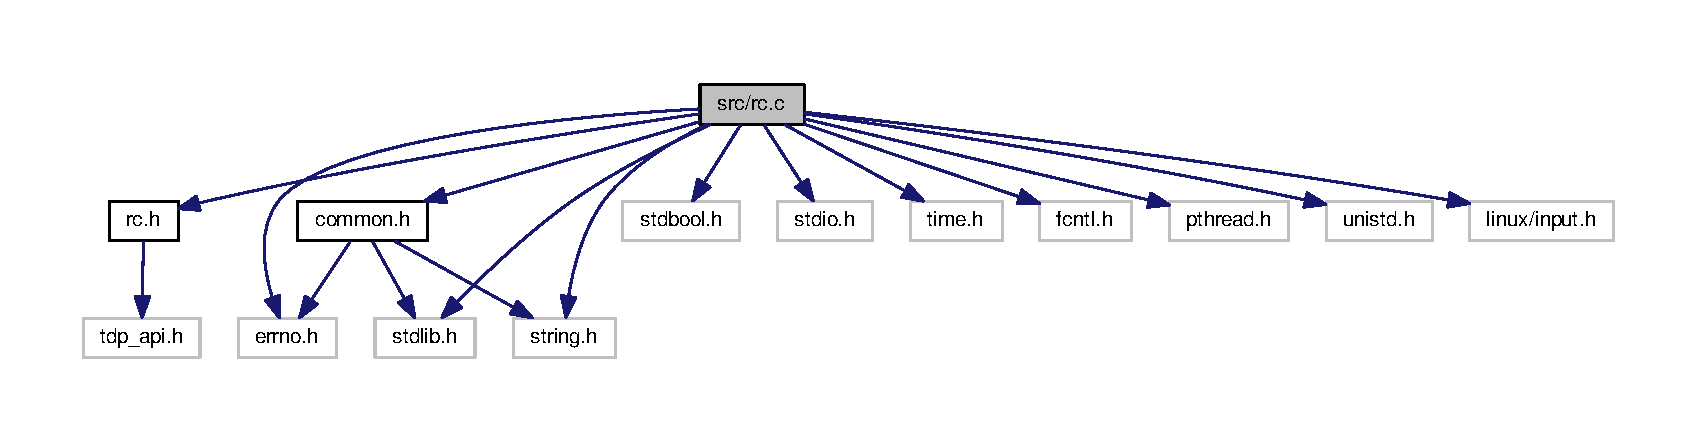
\includegraphics[width=350pt]{rc_8c__incl}
\end{center}
\end{figure}
\subsection*{Data Structures}
\begin{DoxyCompactItemize}
\item 
struct \hyperlink{structargs}{args}
\begin{DoxyCompactList}\small\item\em A shim structure to pass main arguments to Direct\+FB. \end{DoxyCompactList}\end{DoxyCompactItemize}
\subsection*{Macros}
\begin{DoxyCompactItemize}
\item 
\#define {\bfseries \+\_\+\+P\+O\+S\+I\+X\+\_\+\+C\+\_\+\+S\+O\+U\+R\+CE}~200809L\hypertarget{rc_8c_a3024ccd4a9af5109d24e6c57565d74a1}{}\label{rc_8c_a3024ccd4a9af5109d24e6c57565d74a1}

\item 
\#define {\bfseries L\+O\+G\+\_\+\+RC}(fmt, ...)~\hyperlink{common_8h_ac464f11a32500a31842789297a3c31f4}{L\+OG}(\char`\"{}RC\char`\"{}, fmt, \#\#\+\_\+\+\_\+\+V\+A\+\_\+\+A\+R\+G\+S\+\_\+\+\_\+)\hypertarget{rc_8c_a138b57d1bbcd7a781b2b3ab70a1c0076}{}\label{rc_8c_a138b57d1bbcd7a781b2b3ab70a1c0076}

\item 
\#define \hyperlink{rc_8c_a8a2db8e958654a630c12ff9ffa568ea6}{E\+V\+E\+N\+T\+\_\+\+K\+E\+Y\+\_\+\+P\+R\+E\+SS}~1\hypertarget{rc_8c_a8a2db8e958654a630c12ff9ffa568ea6}{}\label{rc_8c_a8a2db8e958654a630c12ff9ffa568ea6}

\begin{DoxyCompactList}\small\item\em Specifies that a key press has occurred. \end{DoxyCompactList}\end{DoxyCompactItemize}
\subsection*{Functions}
\begin{DoxyCompactItemize}
\item 
void \hyperlink{group__rc_ga16d20af699334f6207d806701067ac96}{rc\+\_\+start\+\_\+loop} (const char $\ast$dev, \hyperlink{group__rc_gaa7ca8d3e24ef0c270366ce6fd9bcd258}{rc\+\_\+key\+\_\+callback} kc)
\begin{DoxyCompactList}\small\item\em A function that starts the loop that waits for input events from the remote control. \end{DoxyCompactList}\item 
void \hyperlink{group__rc_ga6d6de982bd06432345e8164a4c453fcc}{rc\+\_\+stop\+\_\+loop} ()
\begin{DoxyCompactList}\small\item\em Stops the event loop. \end{DoxyCompactList}\end{DoxyCompactItemize}


\subsection{Detailed Description}
Contains the implementation of the remote control interface. 


%--- End generated contents ---

% Index
\backmatter
\newpage
\phantomsection
\clearemptydoublepage
\addcontentsline{toc}{chapter}{Index}
\printindex

\end{document}
